\documentclass[a4paper]{ctexrep}
    \usepackage[colorlinks,linkcolor=black]{hyperref}
    \usepackage{listings, geometry, amsmath}
    \usepackage[colorinlistoftodos]{todonotes}
    \usepackage{pifont}
    \usepackage{multirow}  
    \usepackage{amsmath}
    \usepackage{diagbox}
    
    \renewcommand{\multirowsetup}{\centering}
    %\setcounter{chapter}{3}
    \addtocounter{MaxMatrixCols}{15}
    \setlength{\abovecaptionskip}{0pt}
    \setlength{\belowcaptionskip}{10pt}

    \graphicspath{{figures/}} 
    \setmonofont[Mapping={}]{Monaco}	%英文引号之类的正常显示,相当于设置英文字体
    \definecolor{mygreen}{rgb}{0,0.6,0}
    \definecolor{mygray}{rgb}{0.5,0.5,0.5}
    \definecolor{mymauve}{rgb}{0.58,0,0.82}
    \lstset{ % 代码高亮
        backgroundcolor=\color{white},   % choose the background color
        basicstyle=\footnotesize\ttfamily,        % size of fonts used for the code
        columns=fullflexible,
        numbers=left,                    % where to put the line-numbers; possible values are (none, left, right)
        numbersep=0.5em,		% how far the line-numbers are from the code
        breaklines=true,                 % automatic line breaking only at whitespace
        captionpos=t,                    % sets the caption-position to bottom
        tabsize=4,
        frame = single,
        framexleftmargin=2em,
        commentstyle=\color{mygreen},    % comment style
        escapeinside={\%*}{*)},          % if you want to add LaTeX within your code
        keywordstyle=\color{blue},       % keyword style
        stringstyle=\color{mymauve}\ttfamily,     % string literal style
        rulecolor=\color{black},
        % identifierstyle=\color{red},
        language=c++,
        showtabs = false,
        showstringspaces = false,
        showspaces = false,
    }
    
    \geometry{left=3cm,right=3cm,top=3cm,bottom=3cm}
    
    \hypersetup{
        pdftitle={调度实验报告},
        pdfauthor={wdz},
        pdfsubject={实验报告},
        pdfkeywords={},
    }
    
    \ctexset {
        chapter = {
            name = {实验, },
        },
        section = {
            number = \arabic{section},
            format = \Large\bfseries,
        },
        subsection = {
            number = \arabic{section}.\arabic{subsection},
        }
    }
    
    \begin{document}
        \begin{titlepage} % 封面
            \begin{center}
            
\includegraphics[width=12cm]{cover1.eps}\\[1.2cm]
            
\includegraphics[width=5cm]{cover2.png}\\[1.2cm]
            {\zihao{-1} \heiti \textbf{电气信息学院}\\[0.5cm]
            \textbf{调度自动化实验报告}\\[2cm]}
            
            \vspace*{\fill}
            \begin{tabular}{l c}
                \zihao{3}\songti
                专业班级:\quad & \zihao{3}\kaishu{电气工程及其自动化\quad 108班}\\[0.5cm]\zihao{3}\songti
                姓名学号:\quad & \zihao{3}\kaishu{王东泽\quad 2015141441118}\\[0.5cm]\zihao{3}\songti
                %教学班号 xxx\\[0.5cm]\zihao{3}\songti
                任课教师:\quad & \zihao{3}\kaishu{滕欢}\\[0.5cm]\zihao{3}\songti
                指导教师:\quad & \zihao{3}\kaishu{郑秀江}\\[0.5cm]\zihao{3}\songti
                %实验地点 xxx
            \end{tabular}
    
            \vspace*{\fill}
            {\zihao{3} \songti 2017\textasciitilde 2018学年第二学期}\\[0.5cm]
            {\zihao{4} \songti 撰写于\today}
            \end{center}
        \end{titlepage}
    
        \tableofcontents % 目录

        \chapter{电力系统数据采集与实时监控实验}
            \graphicspath{{figures_1/}} 
            \section{实验目的}
                1) 掌握调度自动化仿真实验系统的结构、功能、构成设备。

                2) 掌握数据采集和实时监控 SCADA 的作用、基本功能、实现原理和操作方法。 

                3) 掌握表征发电厂和变电站当前运行状态的参数类型和特点、获取方式、 表现形式。如母线电压、有功功率、无功功率、电流和开关状态等。 

                4) 掌握厂站终端的结构、特点和主要功能。 

                5) 掌握改变发电厂和变电站当前运行方式的控制命令信息的类型和特点、 下发方式。

            \section{原理与说明}
                电力系统是由许多发电厂、输电线路、变电站、配电线路和各种形式的负 荷组成的。电力系统调度中心担负着整个电力网的调度任务,以实现电力系统 的安全优质和经济运行的目标。 
                
                电力系统调度中心必须具有两个功能:第一是与所辖电厂、变电站及上级 调度等进行测量读值、状态信息及控制信号的远距离、高可靠性的双向交换, 简称为电力系统数据采集和监控系统,即 SCADA(Supervisory Control and Data Acquisition);另一个是本身应具有的协调功能(安全监控及其它调度管理与 计划等)。 
                
                \textbf{调度自动化系统结构如图 1.1。}

                \begin{figure}[htbp]
                    \centering
                    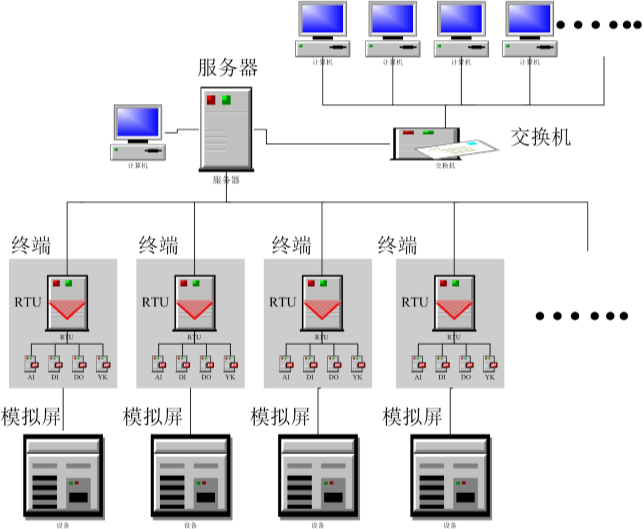
\includegraphics[width=12cm]{1.png}
                    \caption{系统结构图}
                \end{figure}
                
                RTU 结构及技术参数参照《TQDM-II 电力系统综合组态实验系统说明书》。 TQWR-II 微机型 RTU 具有以下特点: 
                
                1、标准的编程语言环境; 
                
                2、极强的环境适应能力,工作温度-40℃-70℃,环境湿度 5\%$\sim$95\%RH; 
                
                3、极强的抗电磁干扰能力; 
                
                4、丰富的通信接口、支持多种通信方式、通信距离长; 
                
                5、大容量存储能力;

                \textbf{通信接口}
                
                两路 RS485 通信接口,可分别响应主机召唤(任一时刻仅一个 RS485 接口 响应主机通讯)。两路 RS485 通信接口都有防雷措施,输入输出之间有光电隔 离器件进行隔离,以保证高质量的通讯传输。 串口通讯初始默认波特率为 9600bps,8 位数据位,1 位停止位,无校验。

                \textbf{遥信 }
                
                本终端有 48 路遥信输入接口,每一路的遥信输入信号都有防雷措施和光电 隔离器件进行保护,保证系统的运行稳定。 用于采集厂站设备运行状态等无源节点,并按规约传送给调度中心,包括: 断路器和隔离刀闸的位置信号、继电保护和自动装置的位置信号、发电机和远 动设备的运行状态等。 
                
                \textbf{遥测 }
                
                本终端共有 48 路电压电流信号输入,用于采集变电所电压、电流、有功功 率、无功功率,功率因数等模拟信号。 
                
                \textbf{遥控 }
                
                本终端有 32 路(对)遥控输出,用于执行调度中心改变设备运行状态的命令,如操作厂站各电压回路的断路器、投切补偿电容和电抗器、发电机组的启停等。为了保证终端遥控的准确性和寿命,本终端的遥控输出均采用松下的继电器。 
                
                \textbf{主要功能 }
                
                1、采集状态量并向远方发送,带有光电隔离,遥信变位优先传送; 
                
                2、采集数据量并向远方发送,带有光电隔离; 
                
                3、直接采集系统工频电量,实现对电压、电流、有功、无功的测量并向远 方发送; 
                
                4、接收并执行遥控及返校; 
                
                5、程序自恢复; 
                
                6、设备自诊断(故障诊断到插件级); 
                
                7、设备自调; 
                
                8、通道监视; 
                
                9、接收并执行遥调; 
                
                10、与两个及两个以上的主站通讯; 
                
                11、采集事件并向远方发送; 
                
                12、提供多个数字接口及多个模拟接口; 
                
                13、可对每个接口特性进行远方/当地设置; 
                
                14、接受远方命令,选择发送各类信息; 
                
                15、当地显示功能,当地接口有隔离器。

            \section{实验项目、方法与要求}
                \subsection{实验系统设备}
                    \textbf{要求: }
                   
                    \textbf{1) 在实验室观察记录调度自动化实验系统由哪些屏柜、设备构成。}
                    
                    \textbf{2) 参考查阅《TQDM-II电力系统综合组态实验系统说明书》,记录每个屏柜 作用、基本功能、重要参数。 实验系统设备分布在实验楼一楼、二楼共三个实验室,系统性地构成调度自动化实验系统。} \\

                    \textbf{发电机组控制屏构成}
                    
                    发电机组控制屏由以下几部分构成: 
                    
                    1) 实验台体 
                    
                    2) 测量表计:励磁电流表、励磁电压表、机端电压表、系统电压表、有功表、 无功表、机端频率表。 
                    
                    3) 一次接线图:发电机组与系统之间的连接示意图。 
                    
                    4) 三相模拟断路器:用三相交流接触器模拟实现 
                    
                    5) 电压互感器:用来采集发电机机端电压和系统电压。 
                    
                    6) 电流互感器:用来采集发电机电流。 
                    
                    7) TQWS-III 微机型自动调速装置:用来调节电动机转速。
                    
                    8) TQWT-III 微机型自动同期装置:实现发电机组与无穷大系统并网操作。 
                    
                    9) TQWL-III 微机型自动励磁装置:用来调节发电机励磁。 
                    
                    10) 励磁整流模块:受自动励磁装置控制输出发电机励磁电压。 
                    
                    11) 调速整流模块:受自动调速装置控制输出调速控制电压。

                    \textbf{系统升压屏构成}
                    
                    系统升压屏由以下几部分构成: 
                   
                    1) 实验台体 
                   
                    2) 测量表计:网络电力表。 
                    
                    3) 一次接线图:系统升压示意图。 
                    
                    4) 三相模拟断路器:用三相交流接触器模拟实现 
                    
                    5) 电压互感器:用来采集变压器高压侧电压和变压器低压侧电压。 
                    
                    6) 电流互感器:用来采集变压器高压侧电流和变压器低压侧电流。
                    
                    系统升压屏工作电源为交流220V 电源。接线端子包括交流 220V 电源进线、 T1 变压器进线、T2 变压器进线、T1 变压器出线、T2 变压器出线、零线、地线等

                \subsection{实验系统体系结构}
                    \textbf{要求: }
                    
                    \textbf{1) 在实验室观察记录调度自动化实验系统体系结构。}
                    
                    \textbf{2) 画出调度自动化实验系统结构如图1.1。 }
                    
                    \textbf{3) 以实验系统为例,分析调度自动化系统体系结构。} \\

                    分别以遥信、遥控,遥调及其主要功能进行说明
                    
                    \textbf{遥信 }
                    
                    本终端有 48 路遥信输入接口,每一路的遥信输入信号都有防雷措施和光电 隔离器件进行保护,保证系统的运行稳定。 
                    
                    用于采集厂站设备运行状态等无源节点,并按规约传送给调度中心,包括: 断路器和隔离刀闸的位置信号、继电保护和自动装置的位置信号、发电机和远 动设备的运行状态等。 
                    
                    \textbf{遥测  }
                    
                    本终端共有 48 路电压电流信号输入,用于采集变电所电压、电流、有功功 率、无功功率,功率因数等模拟信号。 
                    
                    \textbf{遥控 }
                    
                    本终端有 32 路(对)遥控输出,用于执行调度中心改变设备运行状态的命令,如操作厂站各电压回路的断路器、投切补偿电容和电抗器、发电机组的启停等。为了保证终端遥控的准确性和寿命,本终端的遥控输出均采用松下的继电器。 
                    
                    \textbf{主要功能 }
                    
                    1、采集状态量并向远方发送,带有光电隔离,遥信变位优先传送; 
                    
                    2、采集数据量并向远方发送,带有光电隔离; 
                    
                    3、直接采集系统工频电量,实现对电压、电流、有功、无功的测量并向远 方发送; 
                    
                    4、接收并执行遥控及返校; 
                    
                    5、程序自恢复; 
                    
                    6、设备自诊断(故障诊断到插件级); 
                    
                    7、设备自调; 
                    
                    8、通道监视; 
                    
                    9、接收并执行遥调; 
                    
                    10、与两个及两个以上的主站通讯; 
                    
                    11、采集事件并向远方发送; 
                    
                    12、提供多个数字接口及多个模拟接口; 
                    
                    13、可对每个接口特性进行远方/当地设置; 
                    
                    14、接受远方命令,选择发送各类信息; 
                    
                    15、当地显示功能,当地接口有隔离器。

                \subsection{实验一次系统结构}
                    \textbf{要求:}
                    
                    \textbf{1) 画出电力一次系统结构图,标出在实验室构成一次系统时对应的屏柜。}
                    
                    \textbf{2) 在接线屏上完成实验一次系统接线。} 

                    本实验采用‘2MF-无穷大’系统。
                    
                    利用无穷大系统屏、系统升压屏、机组、机组控制屏、变压器屏、网络屏等 构成电网供电系统,利用变电站低压模拟屏、负载屏等构成配电系统。 
                    
                    \textbf{初始状态图如图1.2$\sim$1.13}

                    \begin{figure}[htbp]
                        \centering
                        \begin{minipage}[t]{0.48\textwidth}
                            \centering
                            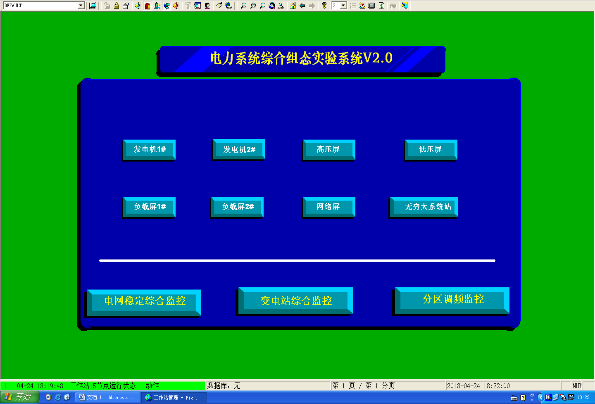
\includegraphics[width=7cm]{3.png}
                            \caption{电力系统综合组态实验系统}
                        \end{minipage} 
                        \begin{minipage}[t]{0.48\textwidth}
                            \centering
                            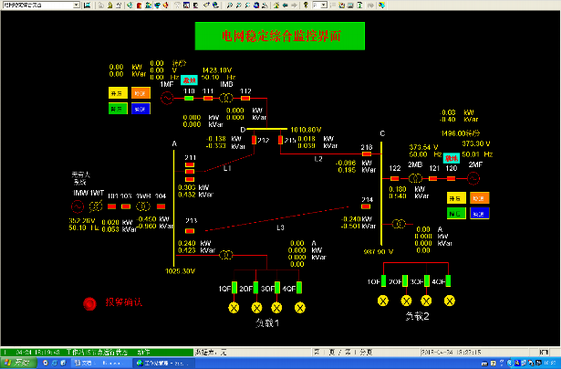
\includegraphics[width=7cm]{4.png}
                            \caption{电网稳定综合监控界面}
                        \end{minipage}
                    \end{figure}

                    \begin{figure}[htbp]
                        \centering
                        \begin{minipage}[t]{0.48\textwidth}
                            \centering
                            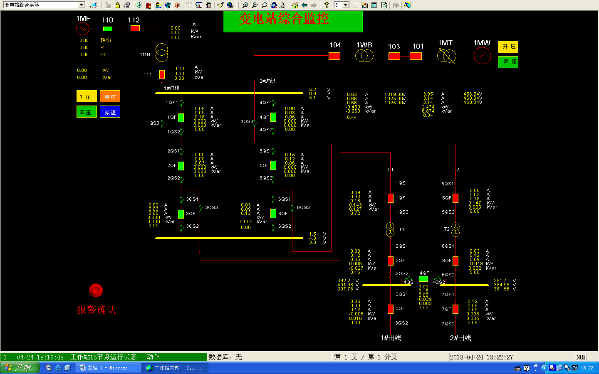
\includegraphics[width=7cm]{5.png}
                            \caption{变压站综合监控}
                        \end{minipage} 
                        \begin{minipage}[t]{0.48\textwidth}
                            \centering
                            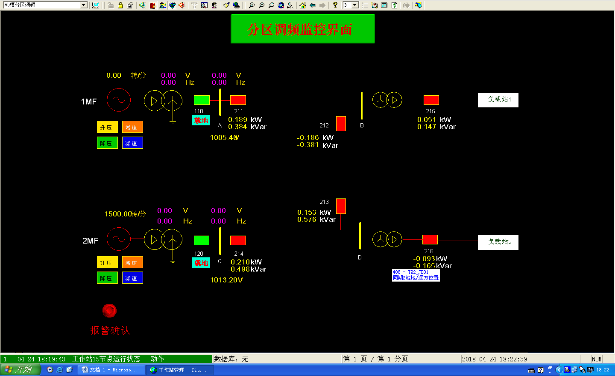
\includegraphics[width=7cm]{6.png}
                            \caption{分区调频监控界面}
                        \end{minipage}
                    \end{figure}

                    \begin{figure}[htbp]
                        \centering
                        \begin{minipage}[t]{0.48\textwidth}
                            \centering
                            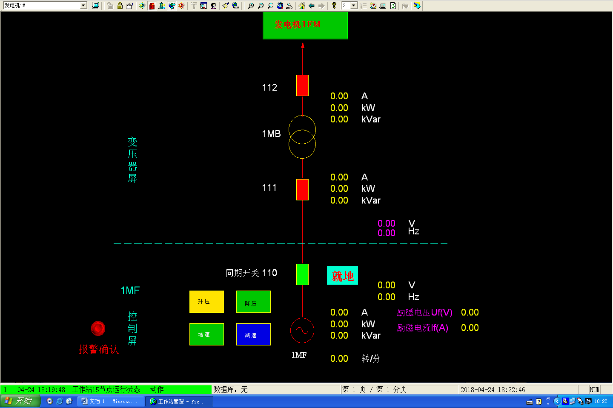
\includegraphics[width=7cm]{7.png}
                            \caption{发电机1FM}
                        \end{minipage} 
                        \begin{minipage}[t]{0.48\textwidth}
                            \centering
                            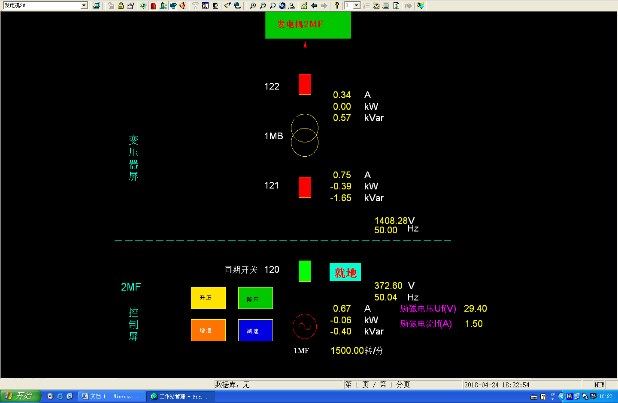
\includegraphics[width=7cm]{8.png}
                            \caption{发电机2FM}
                        \end{minipage}
                    \end{figure}

                    \begin{figure}[htbp]
                        \centering
                        \begin{minipage}[t]{0.48\textwidth}
                            \centering
                            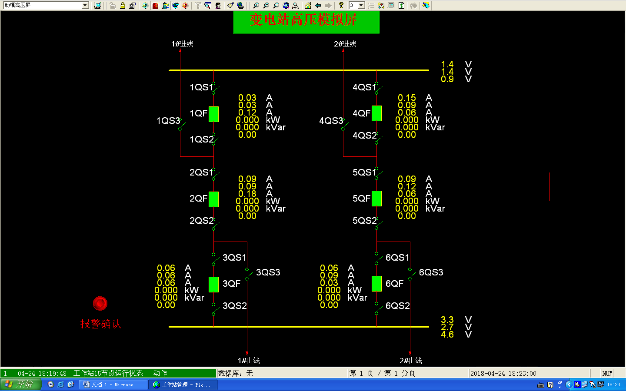
\includegraphics[width=7cm]{9.png}
                            \caption{变电站高压模拟屏}
                        \end{minipage} 
                        \begin{minipage}[t]{0.48\textwidth}
                            \centering
                            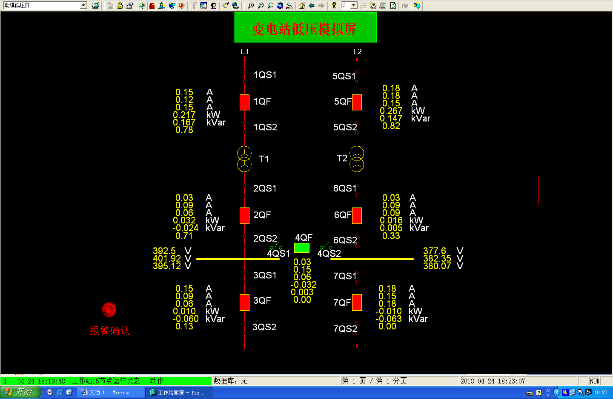
\includegraphics[width=7cm]{10.png}
                            \caption{变电站低压模拟屏}
                        \end{minipage}
                    \end{figure}

                    \begin{figure}[htbp]
                        \centering
                        \begin{minipage}[t]{0.48\textwidth}
                            \centering
                            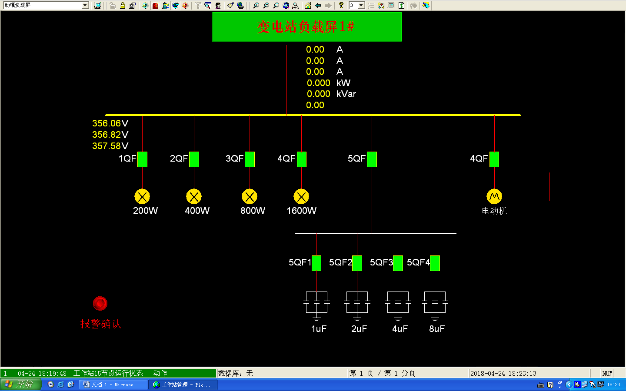
\includegraphics[width=7cm]{11.png}
                            \caption{变电站负载屏1}
                        \end{minipage} 
                        \begin{minipage}[t]{0.48\textwidth}
                            \centering
                            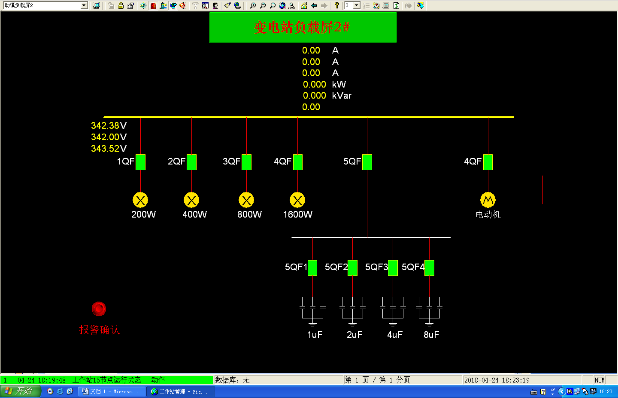
\includegraphics[width=7cm]{12.png}
                            \caption{变电站负载屏2}
                        \end{minipage}
                    \end{figure}

                    \begin{figure}[htbp]
                        \centering
                        \begin{minipage}[t]{0.48\textwidth}
                            \centering
                            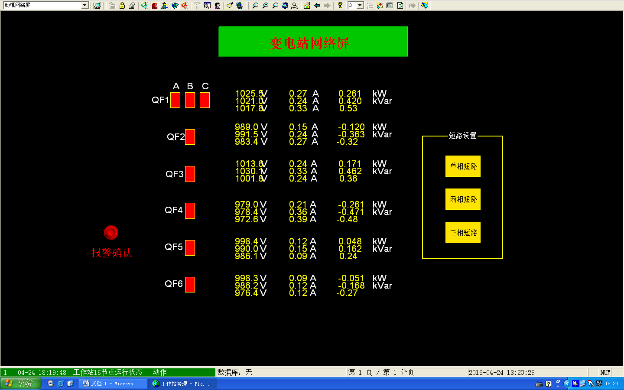
\includegraphics[width=7cm]{13.png}
                            \caption{变电站网络屏}
                        \end{minipage} 
                        \begin{minipage}[t]{0.48\textwidth}
                            \centering
                            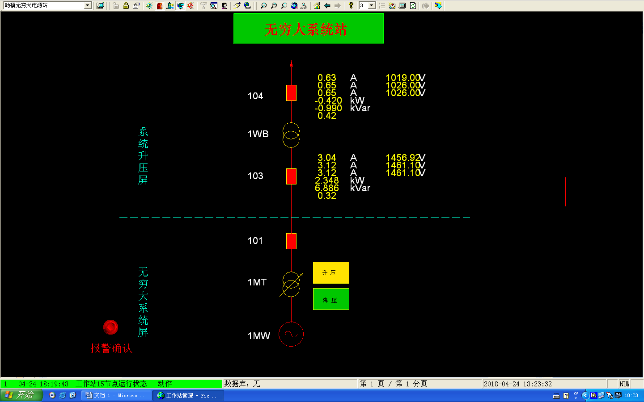
\includegraphics[width=7cm]{14.png}
                            \caption{无穷大系统}
                        \end{minipage}
                    \end{figure}
                
                \newpage

                \subsection{机组并网}
                    \textbf{要求:}

                    \textbf{1) 完成机组并网,使整个系统运行起来。}

                    \textbf{2) 记录实际的并网步骤。} \\

                    \textbf{机组并网步骤参考如下:} 
                    
                    1) 完成实验接线,所有实验接线均在接线屏上实现。
                    
                    2) 断开各机组控制屏上的发电机并列断路器(机组控制屏 1QF)。
                    
                    3) 合上“无穷大系统屏”上的空气开关,使电动调压器带电,通过升压/降压按钮调节调压器输出电压为380V,可通过T1下方的网络电力仪表观察。调节好后合上T1下方断路器,使机组屏上A母线带电。
                    
                    4) 依次合上211、212断路器使D母线带电;合上215、216断路器使C母线带电;合上213、214断路器,构成环网。
                    
                    
                    
                    5) 各机组依次并网。
                    将机组控制屏调速装置打到“自动”位,励磁装置打到“恒 Ug”位,将发  
                    电机组 G1 的频率调到 50Hz 附近,将输出电压调到 380V 左右,同期装置方式选择开关打到“自动”位。在符合并网条件时,同期装置发出合闸信号,并网。
                    
                    按同样方法并入 G2。
                    
                    将各机组控制屏上的自动调速装置“远方/就地”选择开关打到“远方”位,
                    以实现远方调节;将各机组控制屏上的自动励磁装置“远方/就地”选择开关打
                    到“远方”位,以实现远方调节。将各机组控制屏上的自动同期装置“远方/就地”选择开关打到“远方”位,以实现远方调节。

                    \begin{figure}[htbp]
                        \centering
                        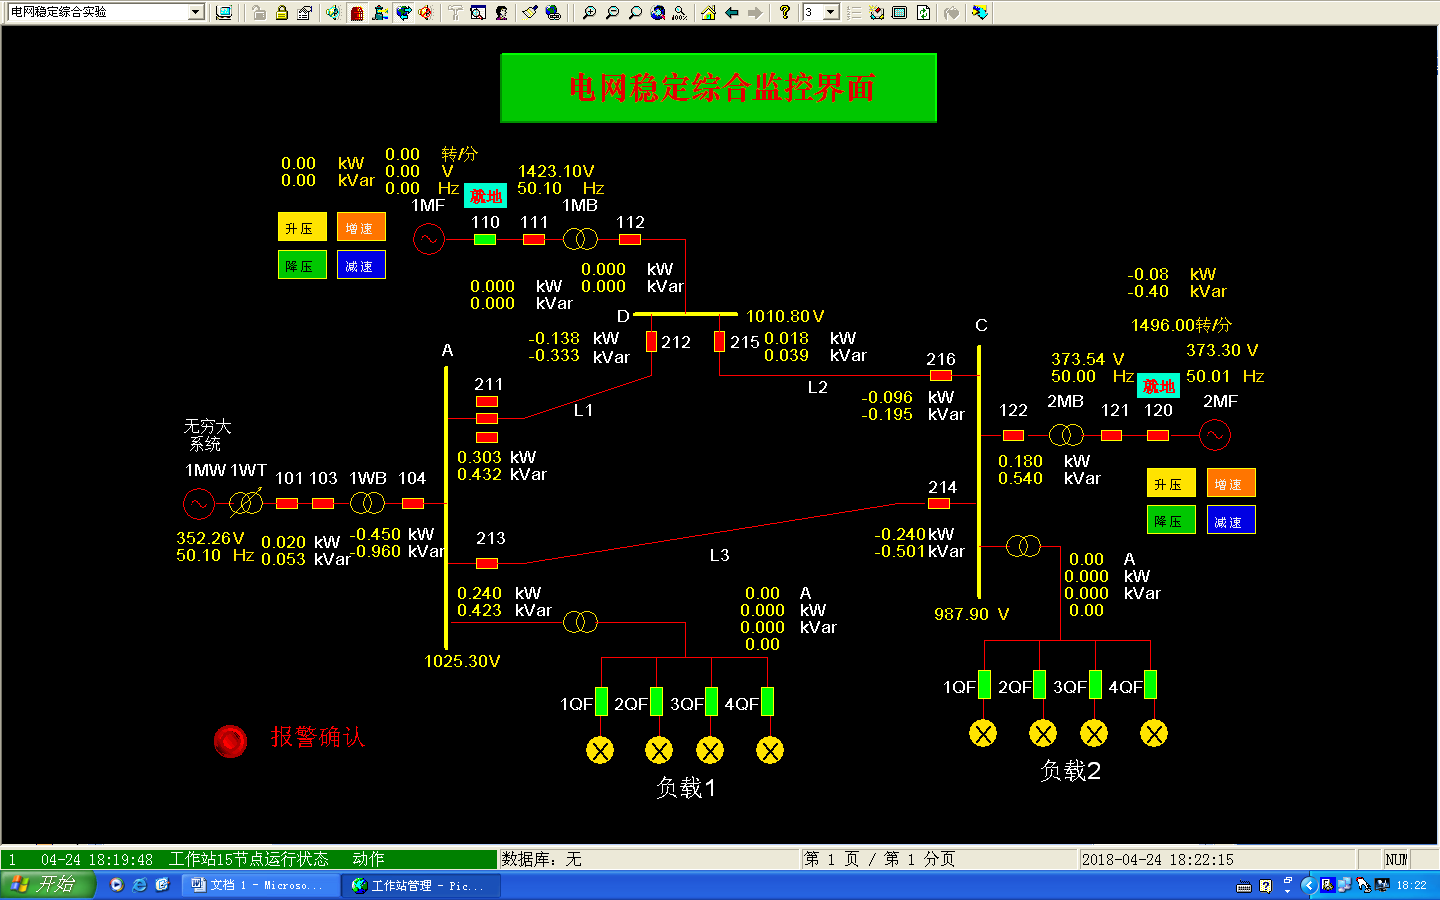
\includegraphics[width=12cm]{15.png}
                        \caption{机组并网后的电网监控界面}
                    \end{figure}

                \subsection{启动主站系统}
                    \textbf{要求:}

                    \textbf{1) 完成主站系统的启动。}

                    \textbf{2) 记录实际的启动步骤,以及观察到的界面。}

                \subsection{遥测、遥信}
                    \textbf{要求:}

                    \textbf{1) 在主站系统,完成遥测、遥信功能。}

                    \textbf{2) 记录实际的操作步骤,记录观察到的界面及遥测、遥信信息,分析遥测、 遥信信息的内容,分析人机接口。} \\

                    \textbf{操作步骤参考如下:}

                    1) 点击系统主界面中的电网稳定综合监控按钮,进入电网稳定综合监控界 面,对整个电网的发电机组、线路、变电站、负荷的潮流分布进行实时监测和观察。 
                    
                    2) 观察记录所有遥测、遥信信息。 
                    
                    3) 点击主接线上方的电网稳定综合监控按钮,可回到系统主界面。 
                    
                    4) 点击系统主界面中的其它按钮,进入其它监控界面,观察记录所有遥测、 遥信信息。
                    
                    初始状态是环网运行,可以在电网稳定综合监控界面及其它屏上记录以下遥测信息,遥信信息主要需要看各个断路器的分合闸状态。

                    \begin{figure}[htbp]
                        \centering
                        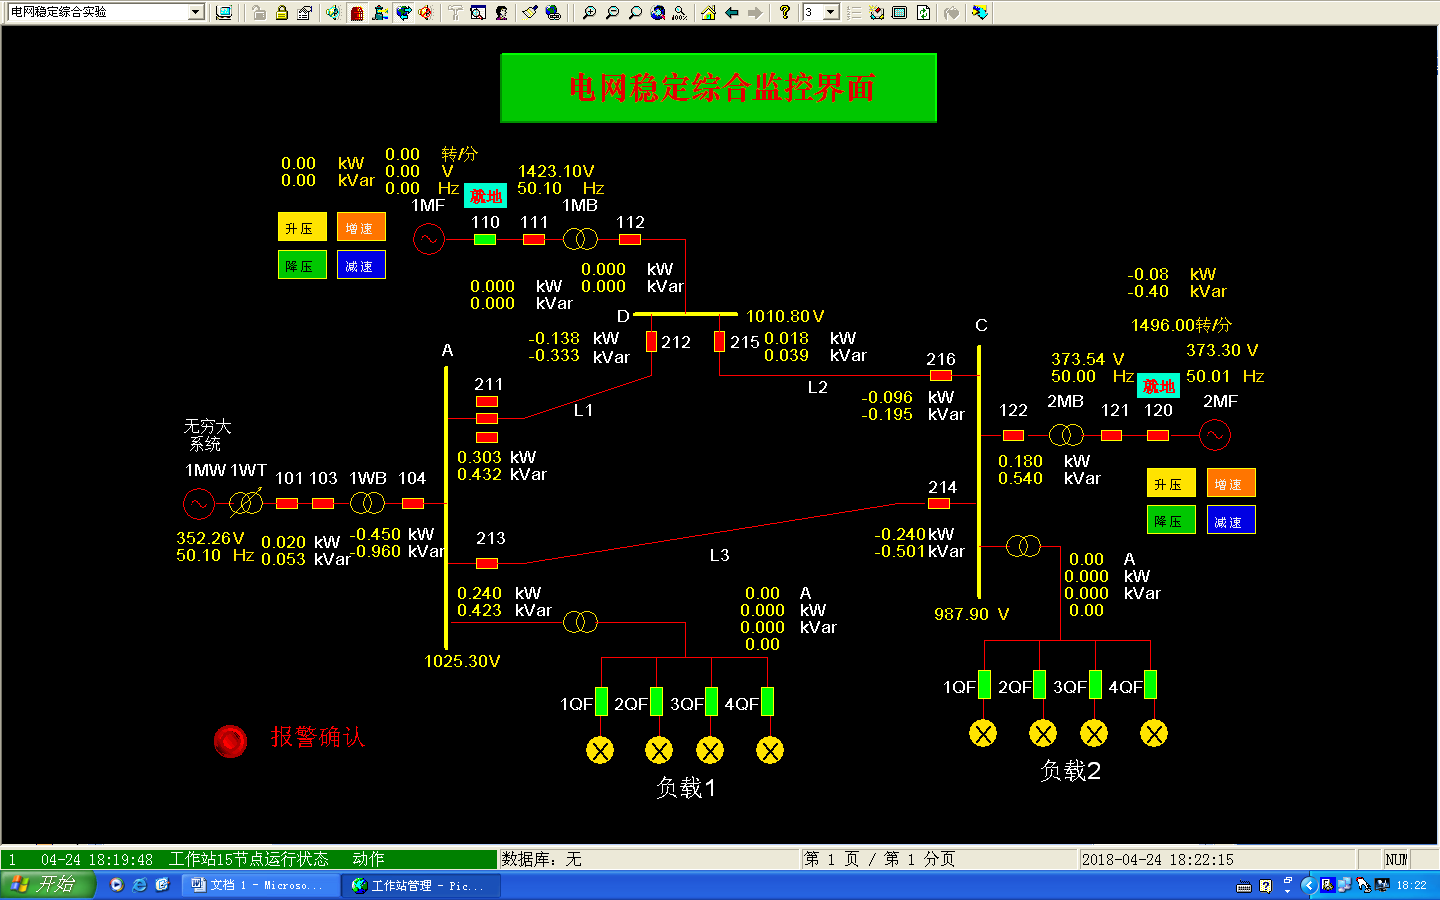
\includegraphics[width=12cm]{16.png}
                        \caption{遥信信息}
                    \end{figure}

                    如图1.15,图中红色的开关代表断路器处于合闸状态,而绿色的代表处于分闸状态,此为遥信信息。遥测信息见表1.1:

                    \begin{table}[htbp]
                        %\hspace{-2.5cm}
                        \centering
                        %\hspace{-5cm}
                        \caption{遥测信息}
                        \centerline
                        {\begin{tabular}{|c|c|c|c|c|c|c|c|c|c|}
                            \hline
                            \diagbox{节点参数}{节点} & G1 & G2 & S无穷大 & 211 & 212 & 213 & 214 & 215 & 216 \\ \hline
                            P(kW) & 0 & -0.08 & 0.020 & 0.303 & -0.138 & 0.240 & -0.240 & 0.018 & -0.096 \\ \hline
                            Q(kVar) & 0 & -0.40 & 0.053 & 0.432 & -0.333 & 0.432 & -0.501 & 0.039 & -0.195 \\ \hline
                            U (V) & 0 & 373.3 & 352.26 & 1025.30 & 1010.80 & 1025.30 & 987.90 & 1010.80 & 987.90 \\ \hline
                            I(A) & 0 & 0.67 & / & / & / & / & / & / & / \\ \hline
                            f(Hz) & 50.01 & 50.10 & / & / & / & / & / & / & / \\
                            \hline
                        \end{tabular}}
                    \end{table}

                \newpage

                \subsection{遥控}
                    \textbf{要求:}
                    
                    \textbf{1) 在主站系统,完成遥控功能。}
                    
                    \textbf{2) 记录实际的遥控操作步骤,记录观察到的界面及遥测、遥信信息,对遥 控操作过程及结果进行分析。} \\

                    遥控操作步骤如下:

                    1) 点击电网稳定综合监控按钮,进入电网稳定综合监控界面。
                    
                    2) 遥控一条输电线路出线断路器分闸、合闸,观察系统潮流变化情况,并做好记录。 
                    
                    3) 遥控负载 1 或负载 2 屏上某断路器分闸、合闸,观察系统潮流变化情况, 并做好记录。 

                    $\bullet$ \quad \textbf{遥控操作:215分闸},如图1.16

                    潮流变化情况(因为尚未涉及到投入电容器,故主要对线路的功率进行记录),数据记录见表1.2

                    \begin{figure}[htbp]
                        \centering
                        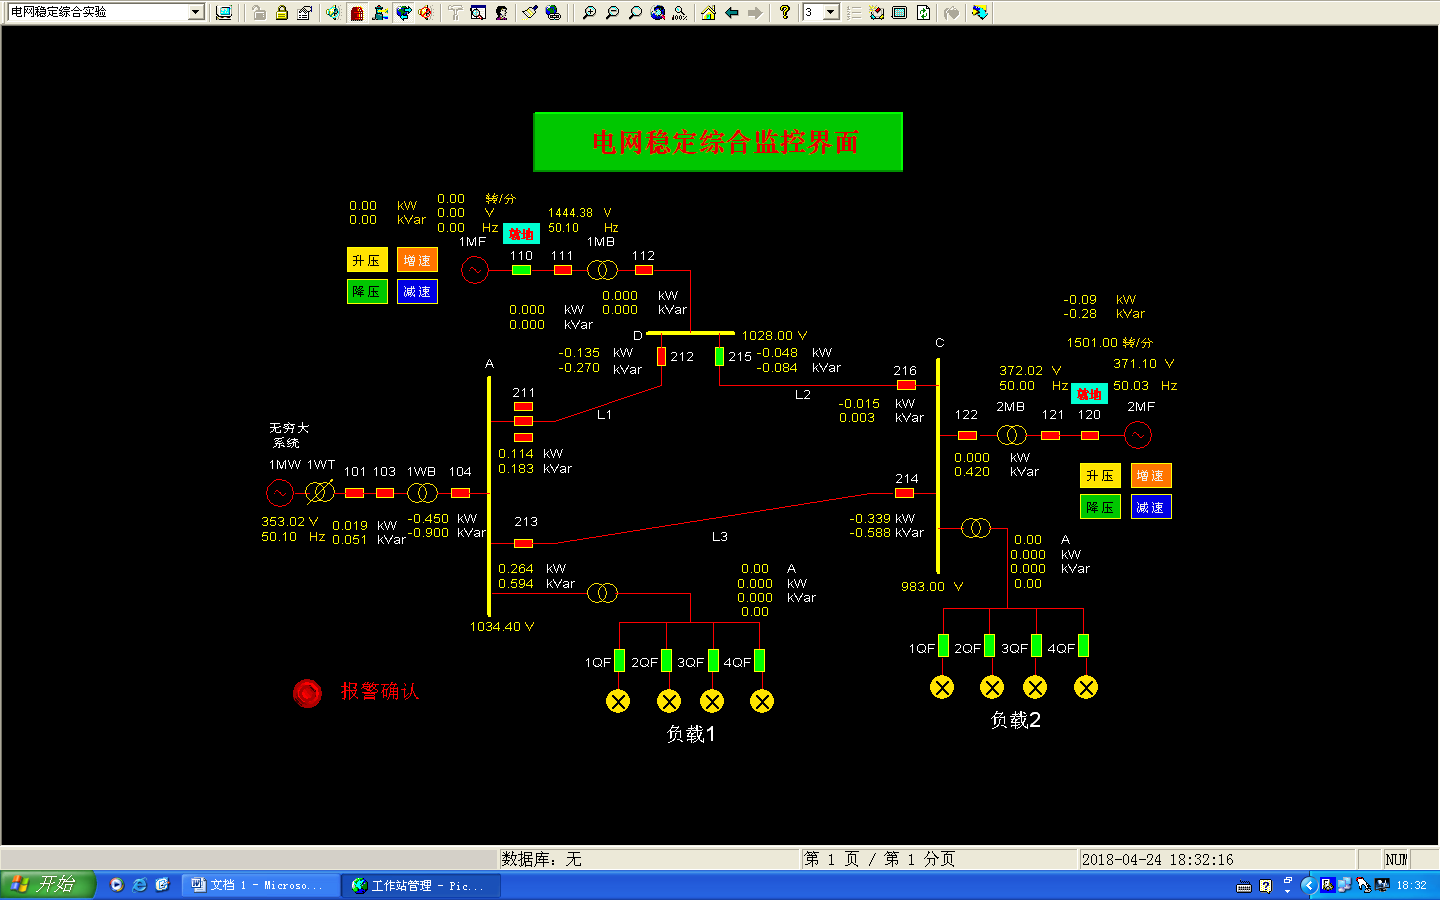
\includegraphics[width=12cm]{17.png}
                        \caption{遥控操作-215分闸}
                    \end{figure}

                    \begin{table}[htbp]
                        \centering
                        \caption{潮流变化情况}
                        \centerline
                        {\begin{tabular}{|c|c|c|c|c|c|c|c|c|c|}
                            \hline
                            \diagbox{节点参数}{节点} & G1 & G2 & S无穷大 & 211 & 212 & 213 & 214 & 215 & 216 \\ \hline
                            P(kW) & 0 & -0.09 & 0.019 & 0.114 & -0.135 & 0.264 & -0.339 & -0.048 & -0.015 \\ \hline
                            Q(kVar) & 0 & -0.28 & 0.051 & 0.183 & -0.27 & 0.549 & -0.588 & -0.084 & 0.003 \\ 
                            \hline
                        \end{tabular}}
                    \end{table}

                    \newpage
                    
                    $\bullet$ \quad \textbf{遥控操作:负载1的QF1合闸},如图1.17

                    潮流变化情况(主要对线路的功率进行记录),数据记录见表1.3

                    \begin{figure}[htbp]
                        \centering
                        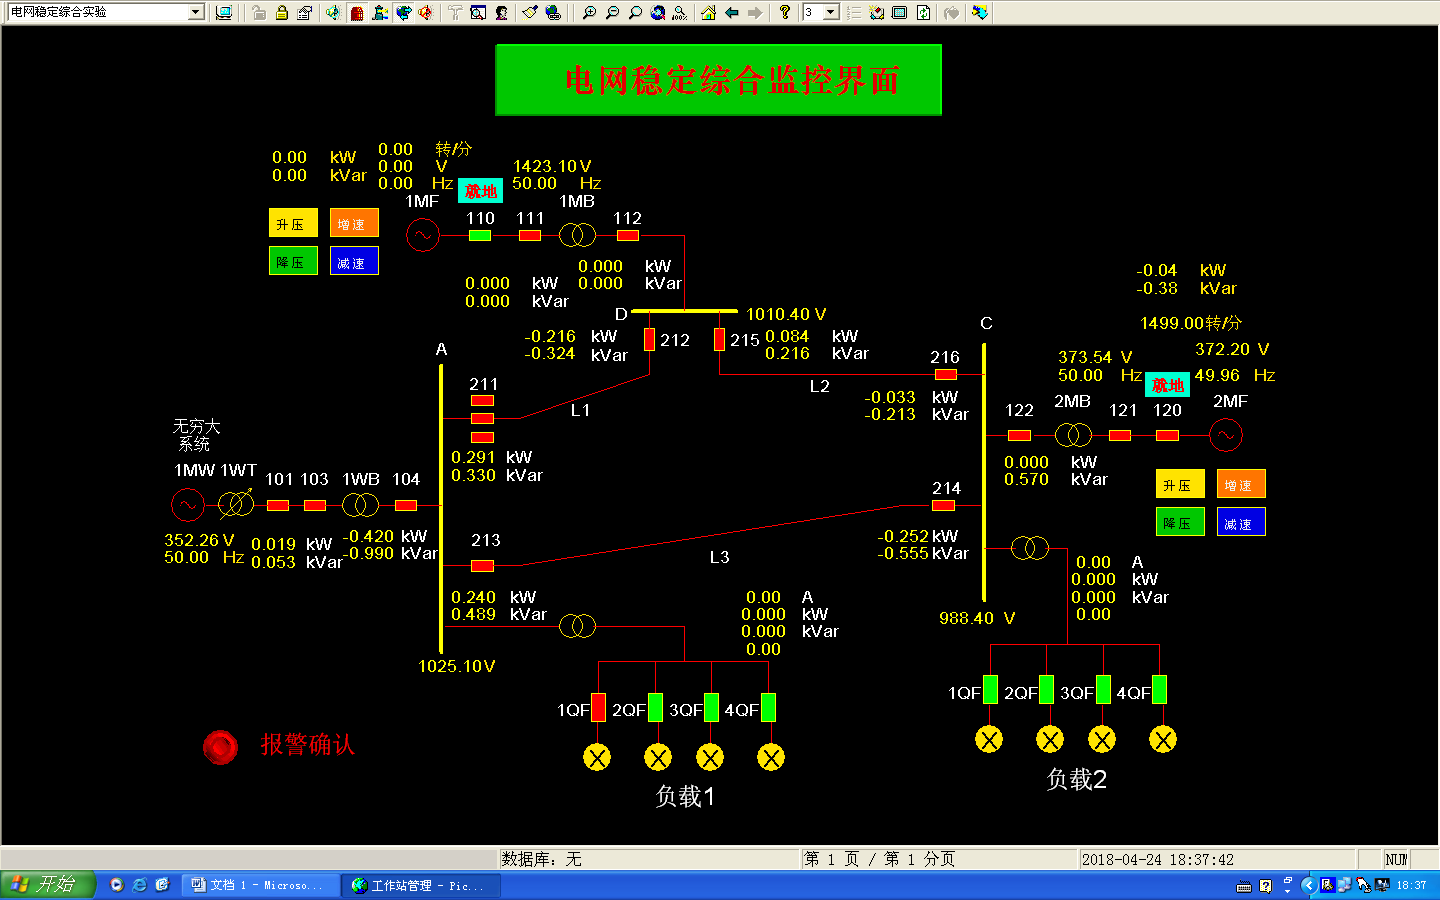
\includegraphics[width=12cm]{18.png}
                        \caption{遥控操作-负载1的QF1合闸}
                    \end{figure}

                    \begin{table}[htbp]
                        \centering
                        \caption{潮流变化情况}
                        \centerline
                        {\begin{tabular}{|c|c|c|c|c|c|c|c|c|c|}
                            \hline
                            \diagbox{节点参数}{节点} & G1 & G2 & S无穷大 & 211 & 212 & 213 & 214 & 215 & 216 \\ \hline
                            P(kW) & 0 & -0.04 & 0.019 & 0.291 & -0.216 & 0.240 & -0.252 & 0.084 & -0.033 \\ \hline
                            Q(kVar) & 0 & -0.38 & 0.053 & 0.330 & -0.324 & 0.489 & -0.555 & 0.216 & -0.213 \\ 
                            \hline
                        \end{tabular}}
                    \end{table}

                    $\bullet$ \quad \textbf{遥控操作:负载1的1QF及负载2的1QF合闸},如图1.18

                    潮流变化情况(主要对线路的功率进行记录),数据记录见表1.4 \\

                    \begin{figure}[htbp]
                        \centering
                        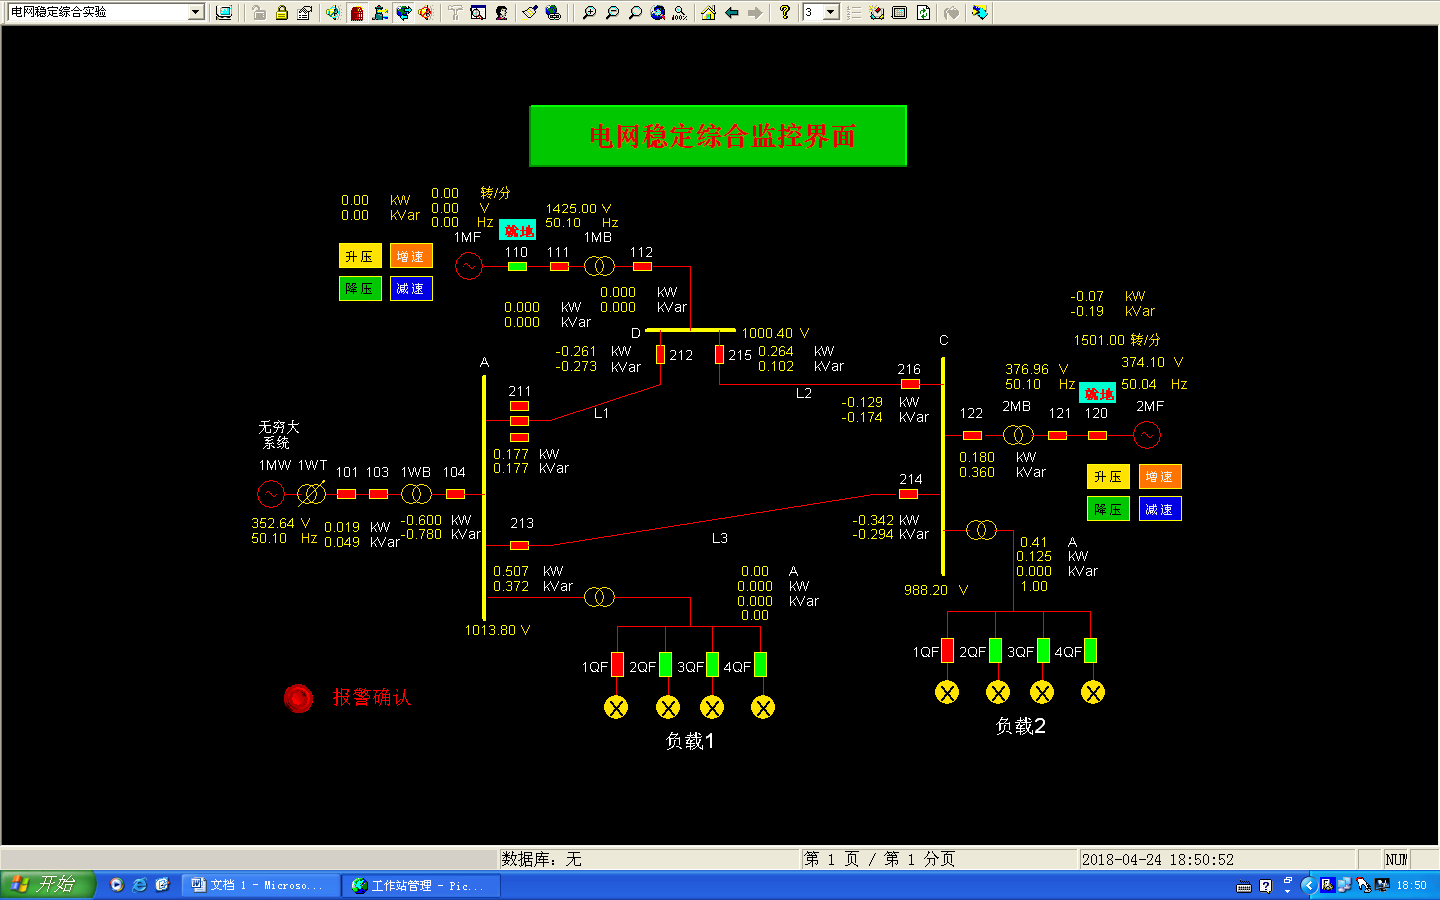
\includegraphics[width=12cm]{19.png}
                        \caption{遥控操作-负载1的1QF及负载2的1QF合闸}
                    \end{figure}

                    \begin{table}[htbp]
                        \centering
                        \caption{潮流变化情况}
                        \centerline
                        {\begin{tabular}{|c|c|c|c|c|c|c|c|c|c|}
                            \hline
                            \diagbox{节点参数}{节点} & G1 & G2 & S无穷大 & 211 & 212 & 213 & 214 & 215 & 216 \\ \hline
                            P(kW) & 0 & -0.07 & -0.60 & 0.177 & -0.261 & 0.507 & -0.342 & 0.264 & -0.129 \\ \hline
                            Q(kVar) & 0 & -0.19 & 0.78 & 0.177 & -0.273 & 0.372 & -0.294 & 0.102 & -0.174 \\ 
                            \hline
                        \end{tabular}}
                    \end{table}

                    \newpage

                    4) 遥控操作时,鼠标移动到断路器位置,鼠标变成※型,点击图标,弹出 操作界面。其详细操作请参照《TQDM-II 电力系统综合组态实验系统说明书》。

                \subsection{遥调}
                    \textbf{要求:}
                    
                    \textbf{1) 在主站系统,完成遥调功能。}
                    
                    \textbf{2) 记录实际的遥调操作步骤,记录观察到的界面及遥测、遥信信息,对遥调操作过程及结果进行分析。}

                    遥调是指对远距离的受控对象的工作状态进行调节的技术,是指在远距离 的情况下,对其所要进行调节的设备的数据进行远距离调控,从而达到想要的 数据效果(如发电机的功率或电压调整,变压器的升降压调节等)。本实验中, 通过遥调发电机原动机的出力和发电机的励磁,改变系统的功率分布和电压。

                    遥调操作步骤如下: 
                    
                    1) 如控制发电机升压,可点击监控界面的“升压”按钮。将鼠标放置于“状态量设置”区的“升压”上,下方的“控制输出”命 令按钮将变为可操作的状态。 点击“控制输出”按钮,弹出如图 1-6 所示的界面,“控制口令”输入 1,并 点击“确认”,弹出如图 1-7 所示的界面,点击“是”确认升压操作,此时监 控系统将向发电机励磁调节装置发送一次升压命令。
                    
                    2) 其他遥调按钮的操作同升压操作一样。 
                    
                    3) 操作监控界面的增速、减速、升压、降压按钮,调节发电机的有功出力、 无功功率和机端电压,同时记录整个系统的潮流。


                    $\bullet$ \quad \textbf{发电机2F升压},升压前如图1.19,升压后如图1.20

                    升压前后系统各参数,升压前数据记录见表1.5,升压后数据记录见表1.6

                    \begin{figure}[htbp]
                        \centering
                        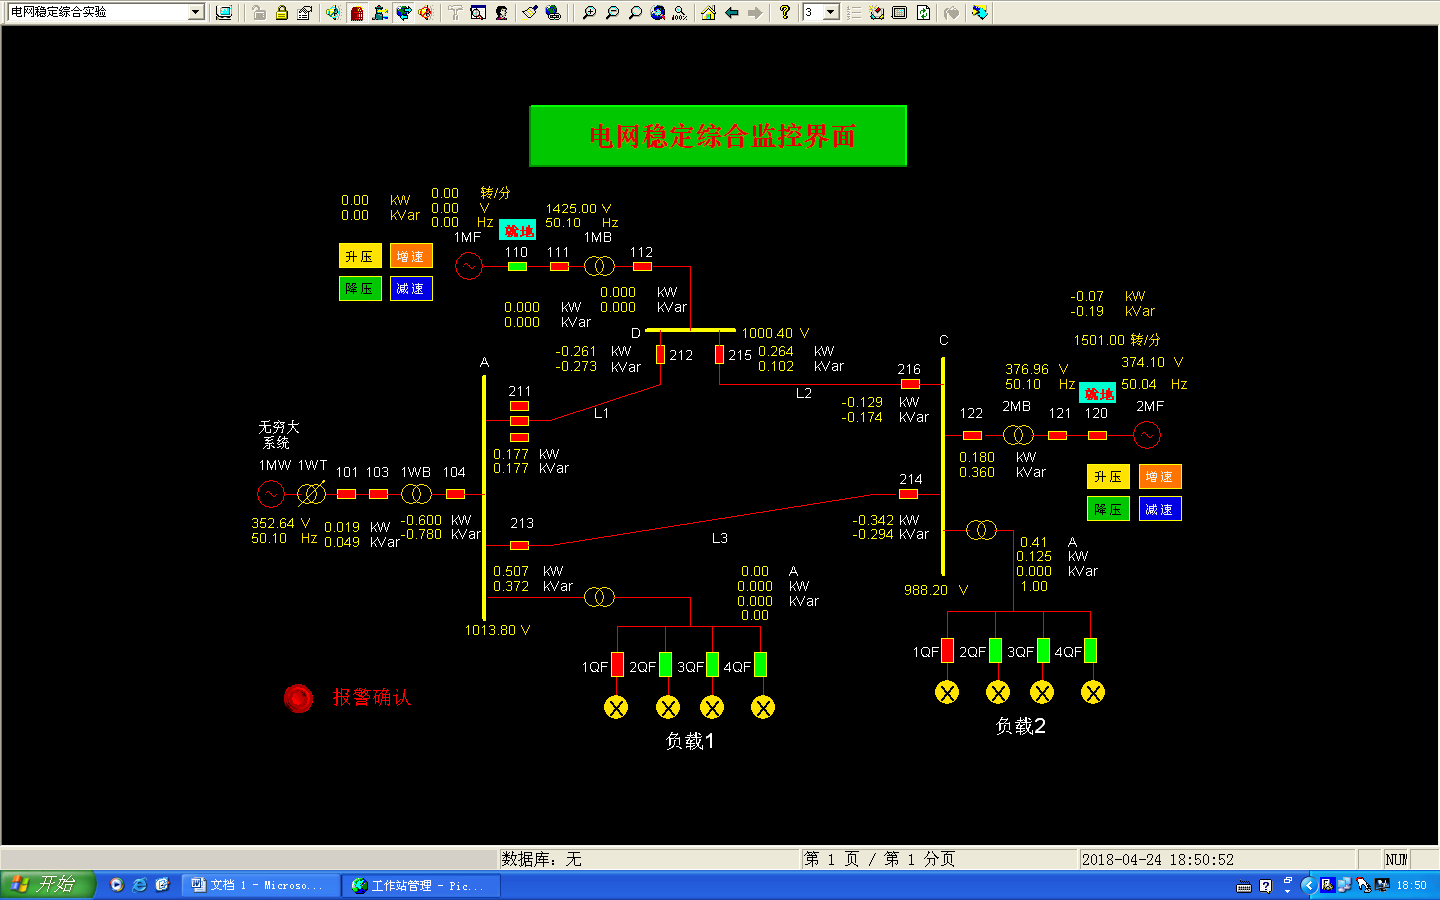
\includegraphics[width=12cm]{20.png}
                        \caption{遥调操作-发电机2F升压前电网监控界面}
                    \end{figure}

                    \begin{table}[htbp]
                        \centering
                        \caption{升压前系统各参数}
                        \centerline
                        {\begin{tabular}{|c|c|c|c|c|c|c|c|c|c|}
                            \hline
                            \diagbox{节点参数}{节点} & G1 & G2 & S无穷大 & 211 & 212 & 213 & 214 & 215 & 216 \\ \hline
                            P(kW) & 0 & -0.07 & -0.60 & 0.177 & -0.261 & 0.507 & -0.342 & 0.264 & -0.129 \\ \hline
                            Q(kVar) & 0 & -0.19 & 0.78 & 0.177 & -0.273 & 0.372 & -0.294 & 0.102 & -0.174 \\ \hline
                            U(V) & 0 & 374.0 & 352.64 & 1013.8 & 1000.4 & 1013.8 & 988.2 & 1000.4 & 988.2 \\
                            \hline
                        \end{tabular}}
                    \end{table}

                    \begin{figure}[htbp]
                        \centering
                        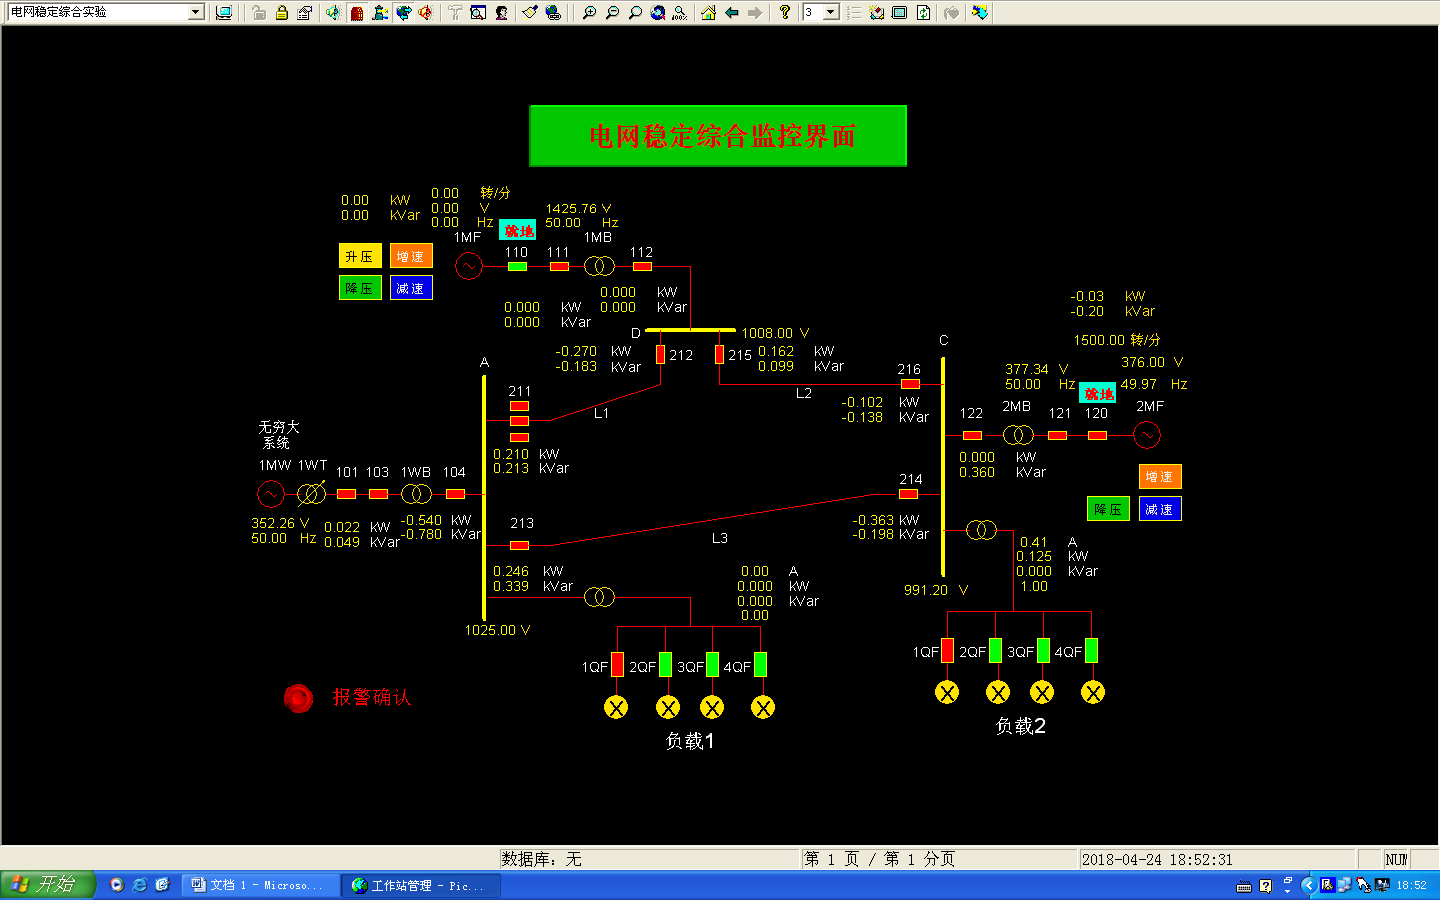
\includegraphics[width=12cm]{21.png}
                        \caption{遥调操作-发电机2F升压后电网监控界面}
                    \end{figure}

                    \begin{table}[htbp]
                        \centering
                        \caption{升压后系统各参数}
                        \centerline
                        {\begin{tabular}{|c|c|c|c|c|c|c|c|c|c|}
                            \hline
                            \diagbox{节点参数}{节点} & G1 & G2 & S无穷大 & 211 & 212 & 213 & 214 & 215 & 216 \\ \hline
                            P(kW) & 0 & -0.03 & 0.022 & 0.210 & -0.270 & 0.246 & -0.363 & 0.162 & -0.102 \\ \hline
                            Q(kVar) & 0 & -0.20 & 0.049 & 0.213 & -0.183 & 0.339 & -0.198 & 0.099 & -0.138 \\ \hline
                            U(V) & 0 & 376.0 & 352.26 & 1025.0 & 1008.0 & 1025.0 & 991.2 & 1008.0 & 991.2 \\ 
                            \hline
                        \end{tabular}}
                    \end{table}

                \newpage

                \subsection{事件记录}
                    \textbf{要求:}

                    \textbf{1) 在主站系统,完成事件记录功能。}

                    \textbf{2) 记录实际的操作步骤,记录观察到的界面及事件记录信息,对事件记录 操作过程及结果进行分析。}

                    当系统有事件发生时,后台监控可简单的记录事件发生的名称和时间,从而使监控人员掌握、了解各个事件发生的具体时间,为各种分析(如保护动作、 误操作等事故分析),提供参考。

                    \textbf{调用事件记录功能操作步骤如下:   }        
                    
                    点击工作站管理栏中事件记录,可弹出实时事件记录界面,记录界面显示事件发生的名称和时间等信息结构和内容。

                \subsection{报警信息}
                    \textbf{要求:}

                    \textbf{1) 在主站系统监控界面,观察记录报警信息,确认并关闭报警。}

                    \textbf{2) 在主站系统监控界面,调用报警信息列表显示功能,记录实际的操作步骤,记录观察到的界面及报警信息。}

                    \textbf{3) 对报警功能操作过程及结果进行分析。} 

                    \textbf{执行报警功能操作步骤参考如下:}

                    1) 当系统有警告事件(如通信故障、断路器变位等)发生时,主站监控界 面上对应的位置将会呈现【红色闪烁】告警状态,表示该位置有事件发生,提 醒操作人员注意。如断路器状态发生变化,则监控画面的该断路器就会闪烁, 提醒操作员注意。 
                    
                    2) 点击工作站管理栏中报警信息,打开系统报警总汇表,报警信息可为各种事故分析,提供有用参考。记录系统报警信息结构 和内容。

                \subsection{其它功能}
                    \textbf{要求:}

                    \textbf{1) 点击工作站管理栏中的其它功能。}

                    \textbf{2) 操作、观察、记录其它功能的实现过程、情况及人机界面。}

                    \textbf{3) 对以上操作过程及结果进行分析。}

                    \textbf{4) 观察、记录 RTU 的配置情况及其所采集的遥测、遥信信息。}

                    \textbf{5) 观察、记录、分析人机数据通信接口。}

                    \textbf{6) 总结分析本实验系统可以实现的主要功能。}

        
        \chapter{电力系统正常运行潮流分布与调整实验}
            \graphicspath{{figures_2/}}
            \section{实验目的}
                1)通过本实验,深入理解潮流分布与调整的相关原理与方法,特别是网络结构变化、机组出力变化、负荷变化、电容器投切等对潮流分布的影响;有功功率与系统频率及无功平衡与系统电压的关系等基本概念和原理。
                
                2)掌握组建仿真实验系统的方法与步骤。 
                
                3)掌握电力调度自动化系统结构、功能。
            
            \section{实验原理与说明}
                电力系统是由许多发电厂,输电线路和各种形式的负荷组成的,在正常运行过程中,绝大多数时间都处于正常运行状态,此时,发电机发出的有功功率和负荷取用的有功功率以及网络损耗的有功功率之间,应随时保持平衡;系统产生的感性无功功率和负荷取用的感性无功功率以及网络损耗的感性无功功率,也随时保持平衡;系统的频率和各母线电压都在规定范围内,各支路潮流都没有超过发热极限值和运行稳定的极限值。但是由于电力系统负荷随时随地都在发生变化,因此系统的发电出力也应随负荷的变化而变化,母线电压和输电线路的潮流也相应发生变化。
                
                电力系统调度中心的任务就是要随时掌握电力系统的实时运行情况,合理 分配各发电厂和线路的潮流,以实现电力系统的安全优质和经济运行的目标。当系统出现异常情况,要根据当时的实际情况,提出决策和措施,指挥控制系统及时动作进行控制,以保证电力系统安全可靠运行。

            \section{实验项目、方法与要求}
                本实验采用‘2MF—无穷大’系统,一次接线图如图2.1。
                
                利用无穷大系统屏、系统升压屏、机组、机组控屏、变压器屏、网络屏等构成电网供电系统,利用变电站低压模拟屏、负载屏、负载等构成配电系统。
                
                图2.1中,断路器对应顺序为:
                
                \begin{center}
                    \begin{tabular}{|c|c|c|c|}
                        \hline
                        断路器编号 & 对应位置 & 断路器编号 & 对应位置 \\ \hline
                        101 & 无穷大系统屏 & 122 & 变压器T2高压侧 \\ \hline
                        103 & 系统升压屏低压侧  & 211 & 网络屏1QF \\ \hline
                        104 & 系统升压屏高压侧 & 212 & 网络屏2QF \\ \hline
                        110 & 1\#机组控制屏1QF & 213 & 网络屏3QF \\ \hline
                        111 & 变压器T1低压侧 & 214 & 网络屏4QF \\ \hline
                        112 & 变压器T1高压侧 & 215 & 网络屏5QF \\ \hline
                        120 & 2\#机组控制屏1QF & 216 & 网络屏6QF \\ \hline
                        121 & 变压器T2低压侧 & & \\
                        \hline
                    \end{tabular}
                \end{center}

                实验接线参照图2.2

                \textbf{注意:接线前务必断开所有电源以及无穷大系统出线开关。}

                A、接线屏上无穷大系统连接至升压变压器入端,升压变压器出端连接网络屏1QF入端,同时将网络屏3QF入端并入1QF入端;
               
                B、1QF出端连接至线路L1入端,线路L1出端连接至2QF入端,2QF出端连接至5QF入端,5QF出端连接至线路L2入端,线路L2出端连接至6QF入端;
                
                C、6QF出端连接至线路4QF出端,3QF出端连接至L3入端,L3出端连接至4QF入端,4QF出端连接至6QF出端;
               
                D、接线屏上机组1连接至变压器T1入端,变压器T1出端连接网络屏5QF入端,同时机组2连接至变压器T2入端,变压器T2出端连接网络屏4QF出端;
                
                E、低压屏进线1连接至3QF入端,低压屏进线2连接至6QF出端;低压屏出线1连接至负载1,低压屏出线2连接至负载2;

                \begin{figure}[htbp]
                    \centering
                    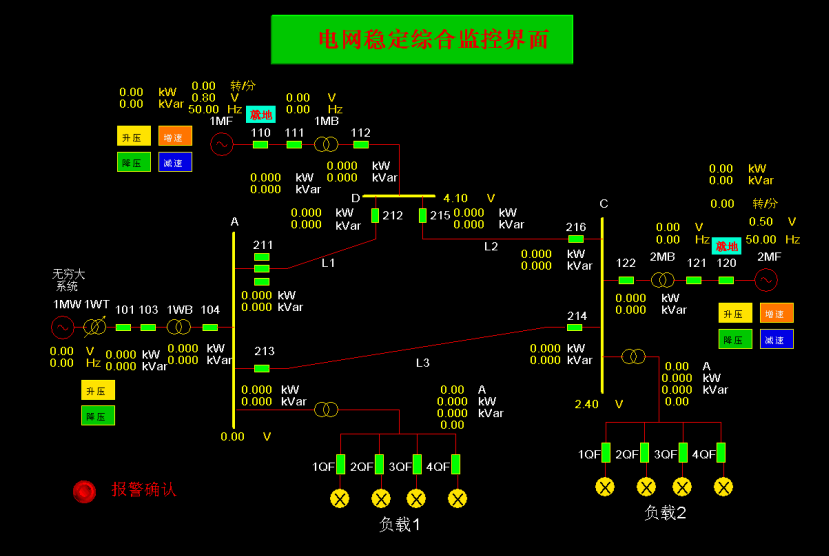
\includegraphics[width=12cm]{1.png}
                    \caption{实验供电系统一次示意图}
                \end{figure}

                \begin{figure}[htbp]
                    \centering
                    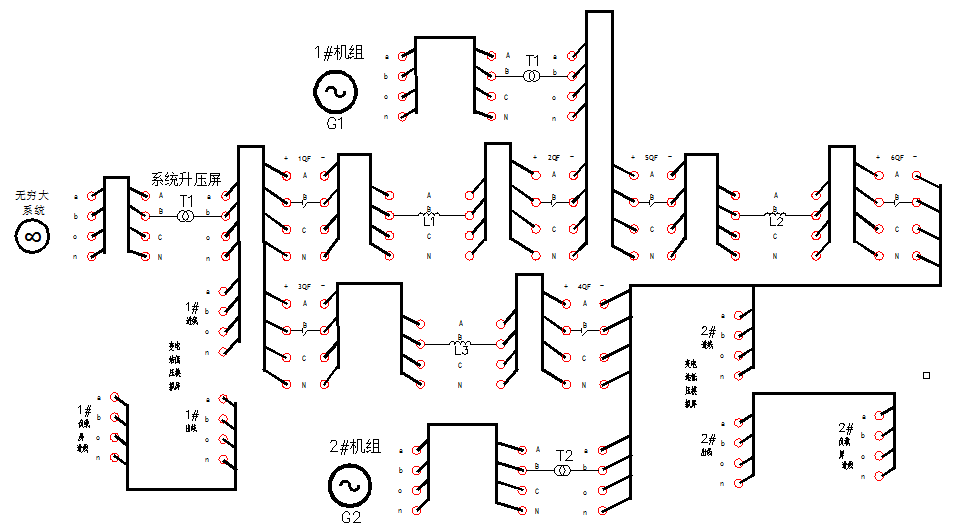
\includegraphics[width=12cm]{2.png}
                    \caption{实验供电系统一次接线图}
                \end{figure}

            \section{不改变网络结构的潮流分布}
                \textbf{注意:}
                
                1) 调节过程中,定子电流不应超过额定值4.61A。
               
                2) 发电机有功功率不应超过2kW。

                \subsection{发电机有功、无功功率改变对系统潮流分布的影响}
                    对发电机2进行升压,降压操作,将数据填入表2.1和表2.2中,并将结果进行比较分析。(在实际实验中,发电机1未接入系统中)

                    \begin{figure}[htbp]
                        \centering
                        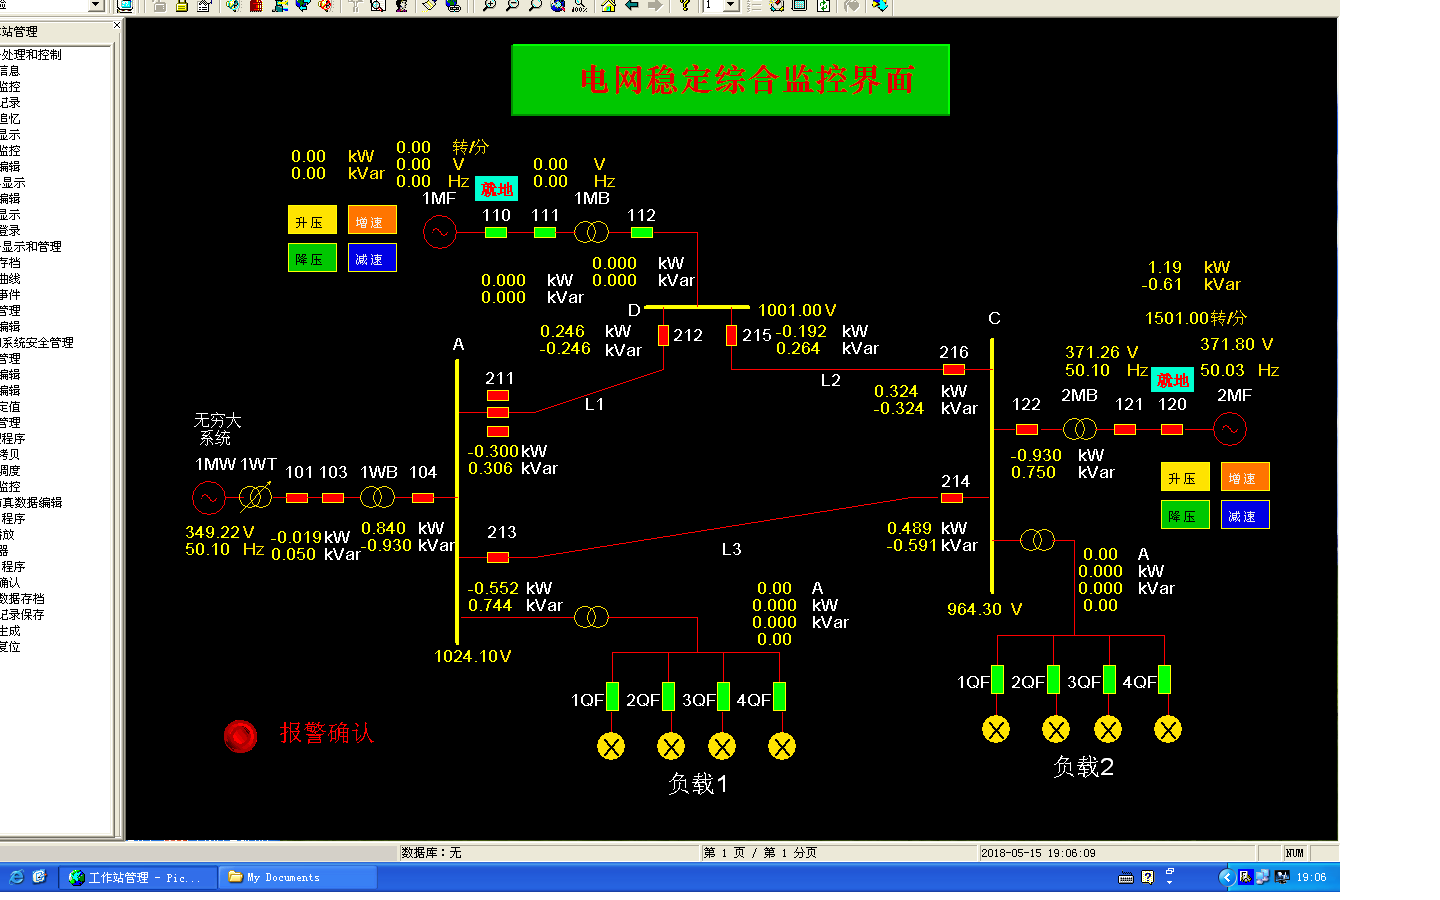
\includegraphics[width=12cm]{3.png}
                        \caption{发电机2升压操作}
                    \end{figure}

                    \begin{figure}[htbp]
                        \centering
                        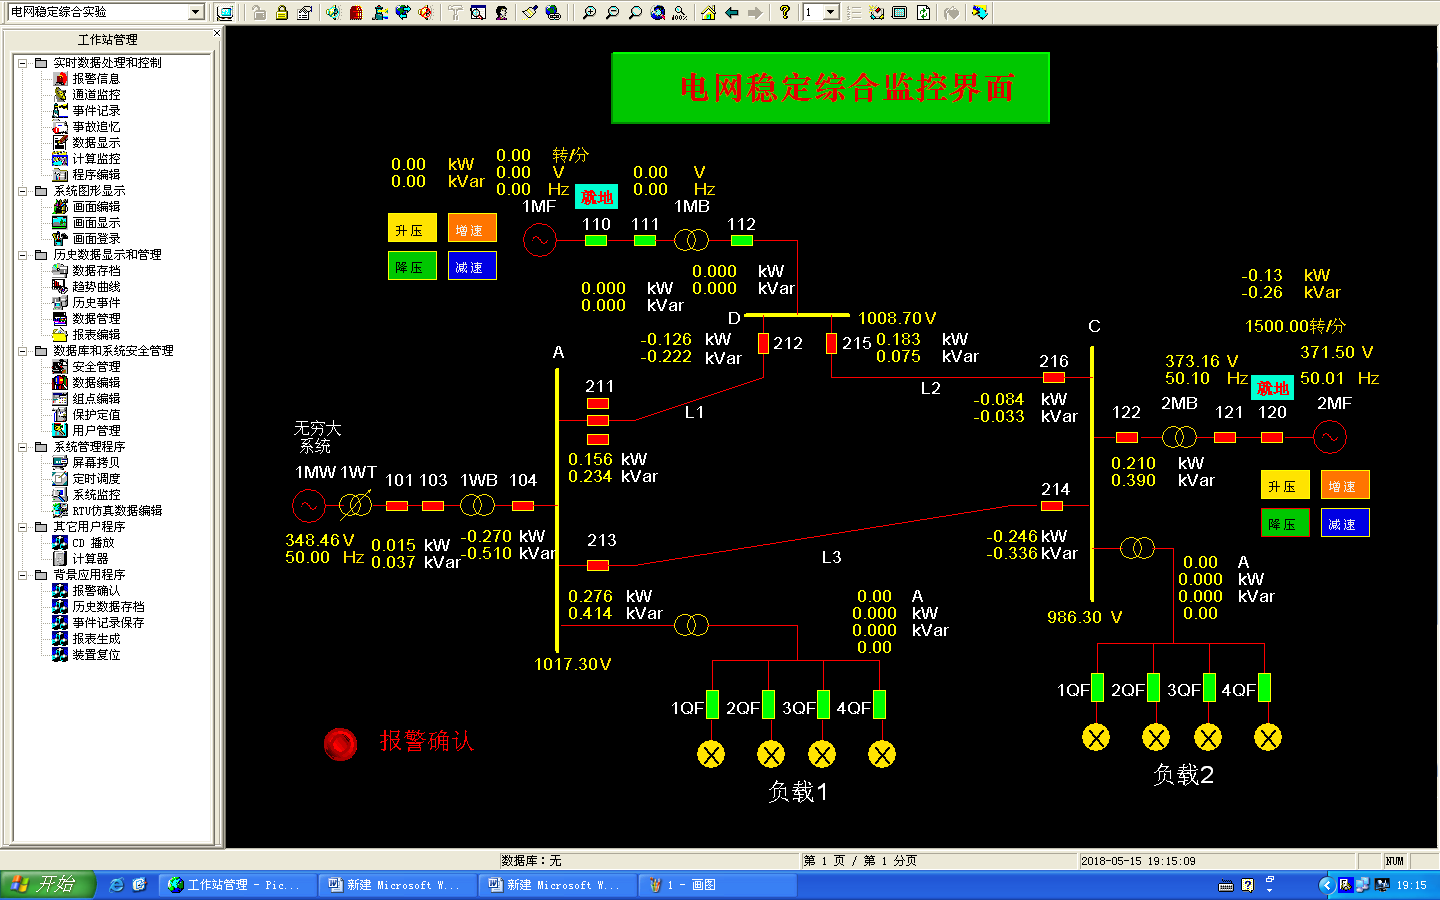
\includegraphics[width=12cm]{4.png}
                        \caption{发电机2降压操作}
                    \end{figure}

                    \begin{table}[htbp]
                        \centering
                        \caption{发电机2升压操作}
                        \centerline
                        {\begin{tabular}{|c|c|c|c|c|c|c|c|c|c|c|}
                            \hline
                            \diagbox{节点参数}{节点} & G1 & G2 & 211 & 212 & 213 & 214 & 215 & 216 & 103 & 104 \\ \hline
                            P(kW) & 0 & 1.19 & -0.3 & 0.246 & -0.552 & 0.489 & -0.192  & 0.324 & -0.019 & 0.84 \\ \hline
                            Q(kVar) & 0 & -0.61 & 0.306 & -0.246 & 0.744 & -0.591 & 0.264 & -0.324 & 0.05 & -0.93 \\ \hline
                            U(V) & 0 & 371.8 & 1024 & 1001 & 1024 & 964.3 & 1001 & 964.3 & 349.22 & 349.22 \\ \hline
                            $cos\varphi$ & 0 & 0.889 & -0.7 & -0.707 & -0.596 & -0.637 & -0.588 & 0.707 & -0.355 & 0.67 \\
                            \hline
                        \end{tabular}}
                    \end{table}

                    \begin{table}[htbp]
                        \centering
                        \caption{发电机2降压操作}
                        \centerline
                        {\begin{tabular}{|c|c|c|c|c|c|c|c|c|c|c|}
                            \hline
                            \diagbox{节点参数}{节点} & G1 & G2 & 211 & 212 & 213 & 214 & 215 & 216 & 103 & 104 \\ \hline
                            P(kW) & 0 & -0.13 & 0.156 & -0.126 & 0.276 & -0.246 & 0.183 & -0.084 & 0.015 & -0.27 \\ \hline
                            Q(kVar) & 0 & -0.26 & 0.234 & -0.222 & 0.414 & -0.336 & 0.075 & -0.033 & 0.037 & -0.51 \\ \hline
                            U(V) & 0 & 371.5 & 1017.3 & 1008.7 & 1017.3 & 986.3 & 1008.7 & 986.3 & 348.46 & 348.46 \\ \hline
                            $cos\varphi$ & 0 & -0.447 & 0.555 & -0.494 & 0.555 & -0.591 & 0.925 & -0.931 & 0.376 & -0.468 \\
                            \hline
                        \end{tabular}}
                    \end{table}

                \subsection{切负荷对系统潮流分布的影响}
                    通过控制低压屏、负载屏上断路器,投/切阻性负载,观察各参数的变化,并记录于表2.4和表2.5中,对数据进行比较分析。
                    
                    首先对负载1的1QF进行投入操作,然后对负载2的3QF进行投入操作,使负载1的200W负荷和负载2的800W负荷接入系统中。

                    \begin{figure}[htbp]
                        \centering
                        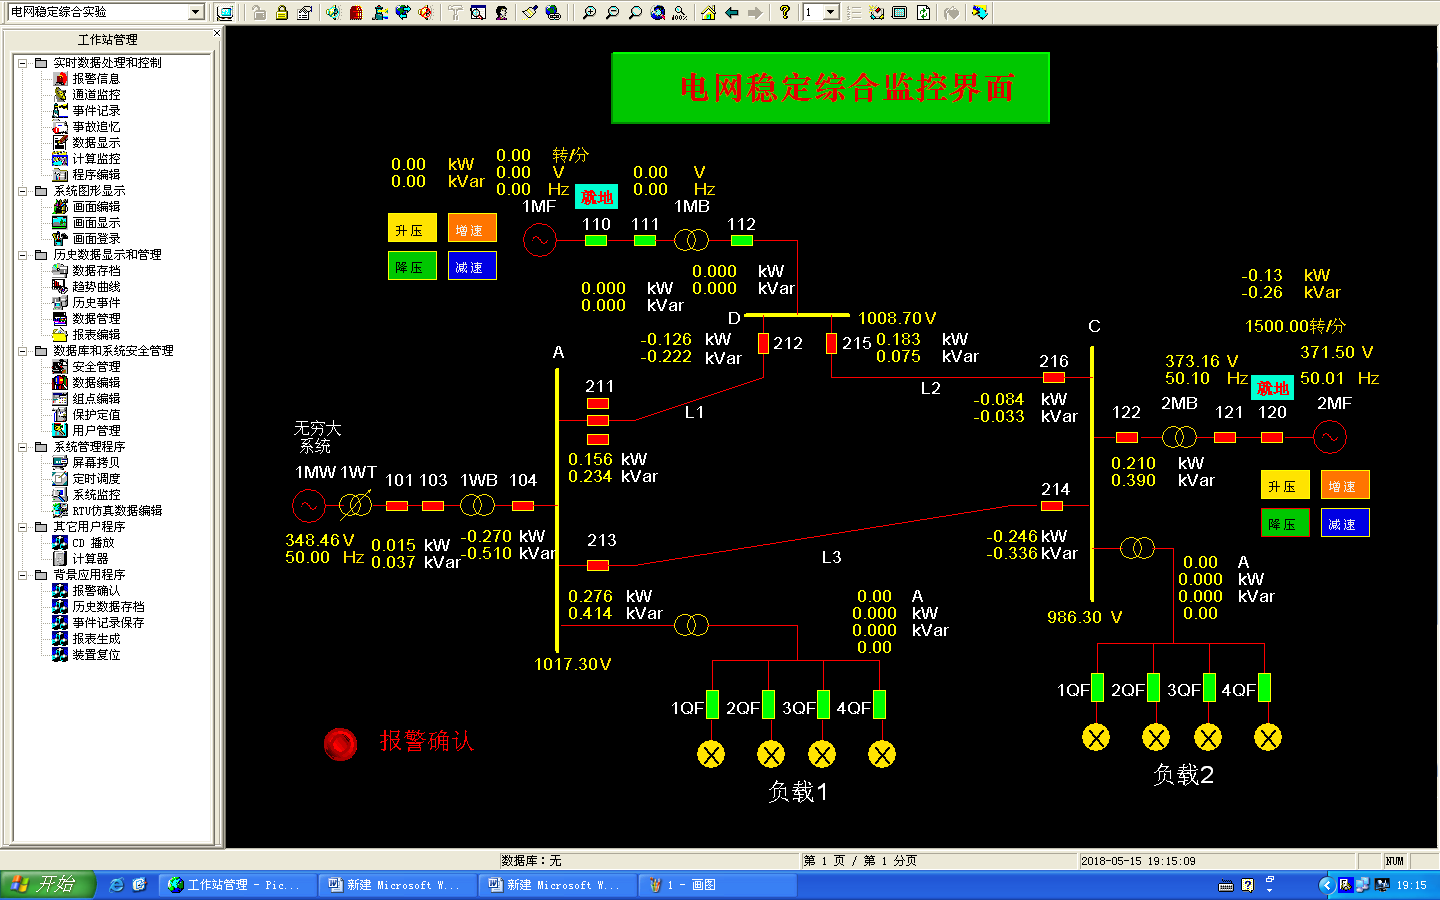
\includegraphics[width=12cm]{5.png}
                        \caption{投入负荷前}
                    \end{figure}

                    \begin{figure}[htbp]
                        \centering
                        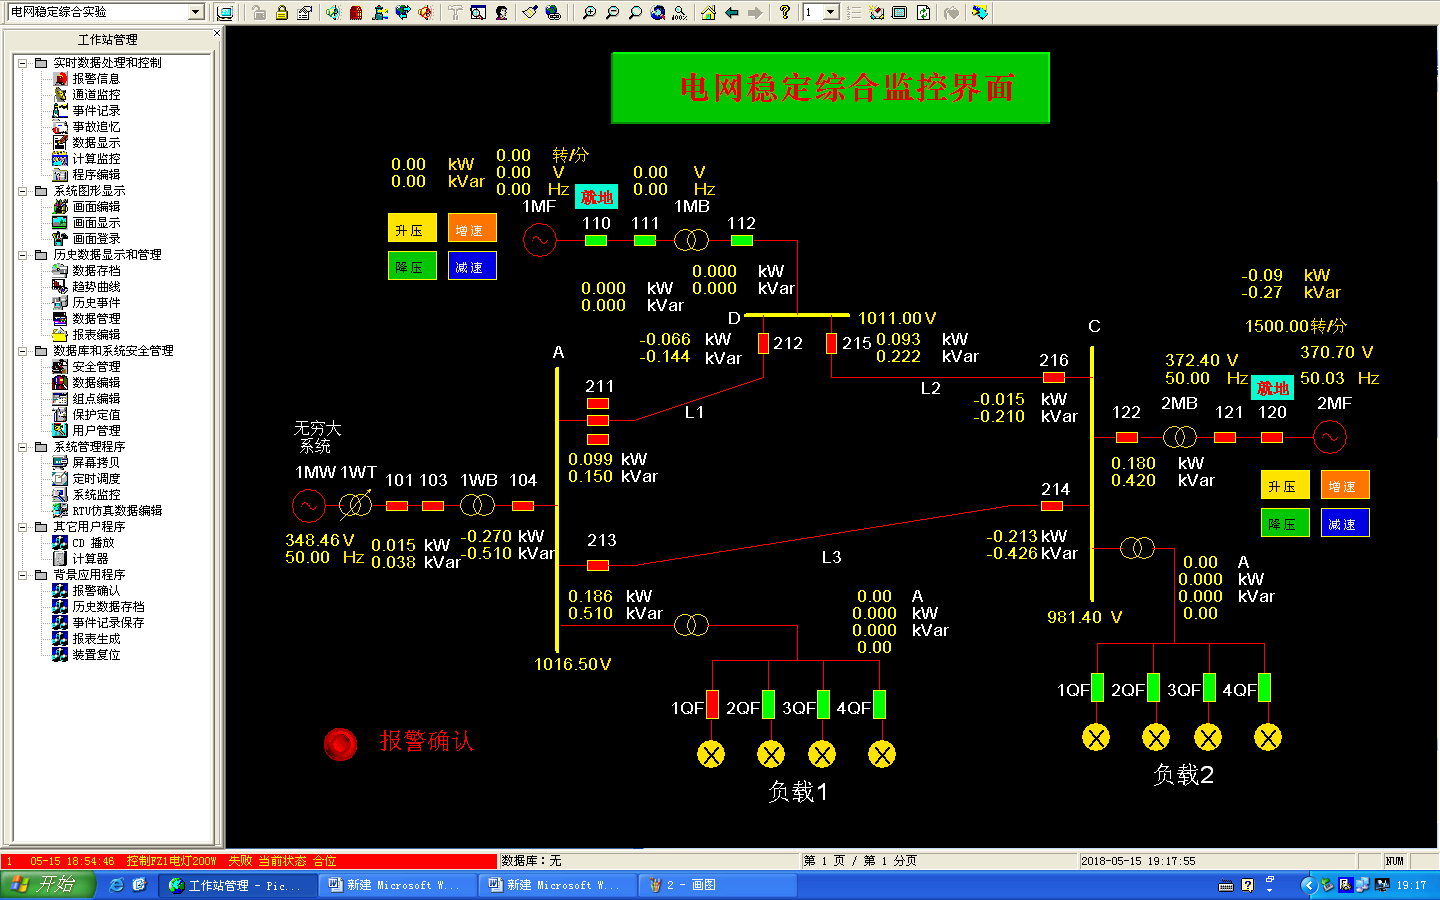
\includegraphics[width=12cm]{6.png}
                        \caption{投入负载1的200W负荷}
                    \end{figure}

                    \begin{figure}[htbp]
                        \centering
                        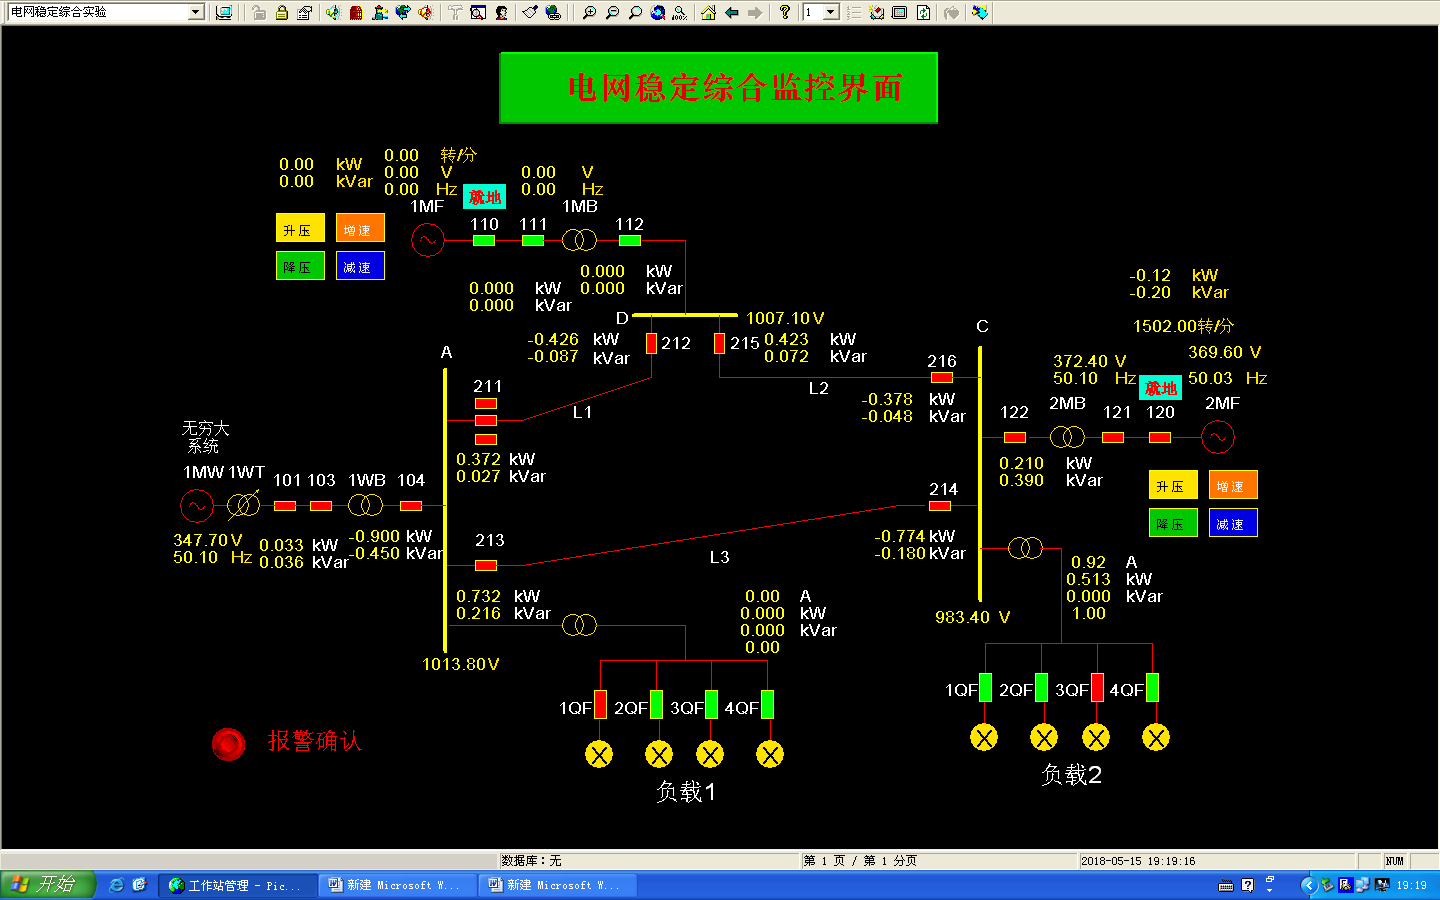
\includegraphics[width=12cm]{7.png}
                        \caption{投入负载2的800W负荷}
                    \end{figure}

                    \begin{table}[htbp]
                        \centering
                        \caption{投入负荷前}
                        \centerline
                        {\begin{tabular}{|c|c|c|c|c|c|c|c|c|c|c|}
                            \hline
                            \diagbox{节点参数}{节点} & G1 & G2 & 211 & 212 & 213 & 214 & 215 & 216 & 103 & 104 \\ \hline
                            P(kW) & 0 & -0.13 & 0.156 & -0.126 & 0.276 & -0.246 & 0.183 & -0.084 & 0.015 & -0.27 \\ \hline
                            Q(kVar) & 0 & -0.26 & 0.234 & -0.222 & 0.414 & -0.336 & 0.075 & -0.033 & 0.037 & -0.51  \\ \hline
                            U(V) & 0 & 371.5 & 1017.3 & 1008.7 & 1017.3 & 986.3 & 1008.7 & 986.3 & 348.46 & 348.46 \\ \hline
                            $cos\varphi$ & 0 & -0.447 & 0.555 & -0.494 & 0.555 & -0.591 & 0.925 & -0.931 & 0.376 & -0.468 \\
                            \hline
                        \end{tabular}}
                    \end{table}

                    \begin{table}[htbp]
                        \centering
                        \caption{投入负载1的200W负荷后}
                        \centerline
                        {\begin{tabular}{|c|c|c|c|c|c|c|c|c|c|c|}
                            \hline
                            \diagbox{节点参数}{节点} & G1 & G2 & 211 & 212 & 213 & 214 & 215 & 216 & 103 & 104 \\ \hline
                            P(kW) & 0 & -0.09 & 0.372 & -0.066 & 0.186 & -0.213 & 0.093 & -0.015 & 0.015 & -0.27 \\ \hline
                            Q(kVar) & 0 & -0.27 & 0.15 & -0.144 & 0.51 & -0.426 & 0.222 & -0.21 & 0.038 & -0.51 \\ \hline
                            U(V) & 0 & 370.7 & 1016.5 & 1011 & 1016.5 & 981.4 & 1011 & 981.4 & 348.46 & 348.46 \\ \hline
                            $cos\varphi$ & 0 & -0.316 & 0.927 & -0.417 & 0.343 & -0.447 & 0.386 & -0.071 & 0.367 & -0.468 \\
                            \hline
                        \end{tabular}}
                    \end{table}

                    \begin{table}[htbp]
                        \centering
                        \caption{投入负载2的800W负荷后}
                        \centerline
                        {\begin{tabular}{|c|c|c|c|c|c|c|c|c|c|c|}
                            \hline
                            \diagbox{节点参数}{节点} & G1 & G2 & 211 & 212 & 213 & 214 & 215 & 216 & 103 & 104 \\ \hline
                            P(kW) & 0 & -0.12 & 0.372 & -0.426 & 0.732 & -0.774 & 0.423 & -0.378 & 0.033 & -0.9 \\ \hline
                            Q(kVar) & 0 & -0.2 & 0.027 & -0.087 & 0.216 & -0.18 & 0.072 & -0.048 & 0.036 & -0.45 \\ \hline
                            U(V) & 0 & 369.6 & 1013.8 & 1007.1 & 1013.8 & 983.4 & 1007.1 & 983.4 & 347.7 & 347.7 \\ \hline
                            $cos\varphi$ & 0 & -0.515 & 0.997 & -0.98 & 0.959 & -0.974 & 0.986 & -0.992 & 0.676 & -0.894 \\
                            \hline
                        \end{tabular}}
                    \end{table}
                
                \newpage
                
                \subsection{投、切电容器对潮流分布的影响}
                    投、切电容器观察各参数的变化,并记录数据于表2.6和表2.7中,对数据进行比较分析。

                    \begin{figure}[htbp]
                        \centering
                        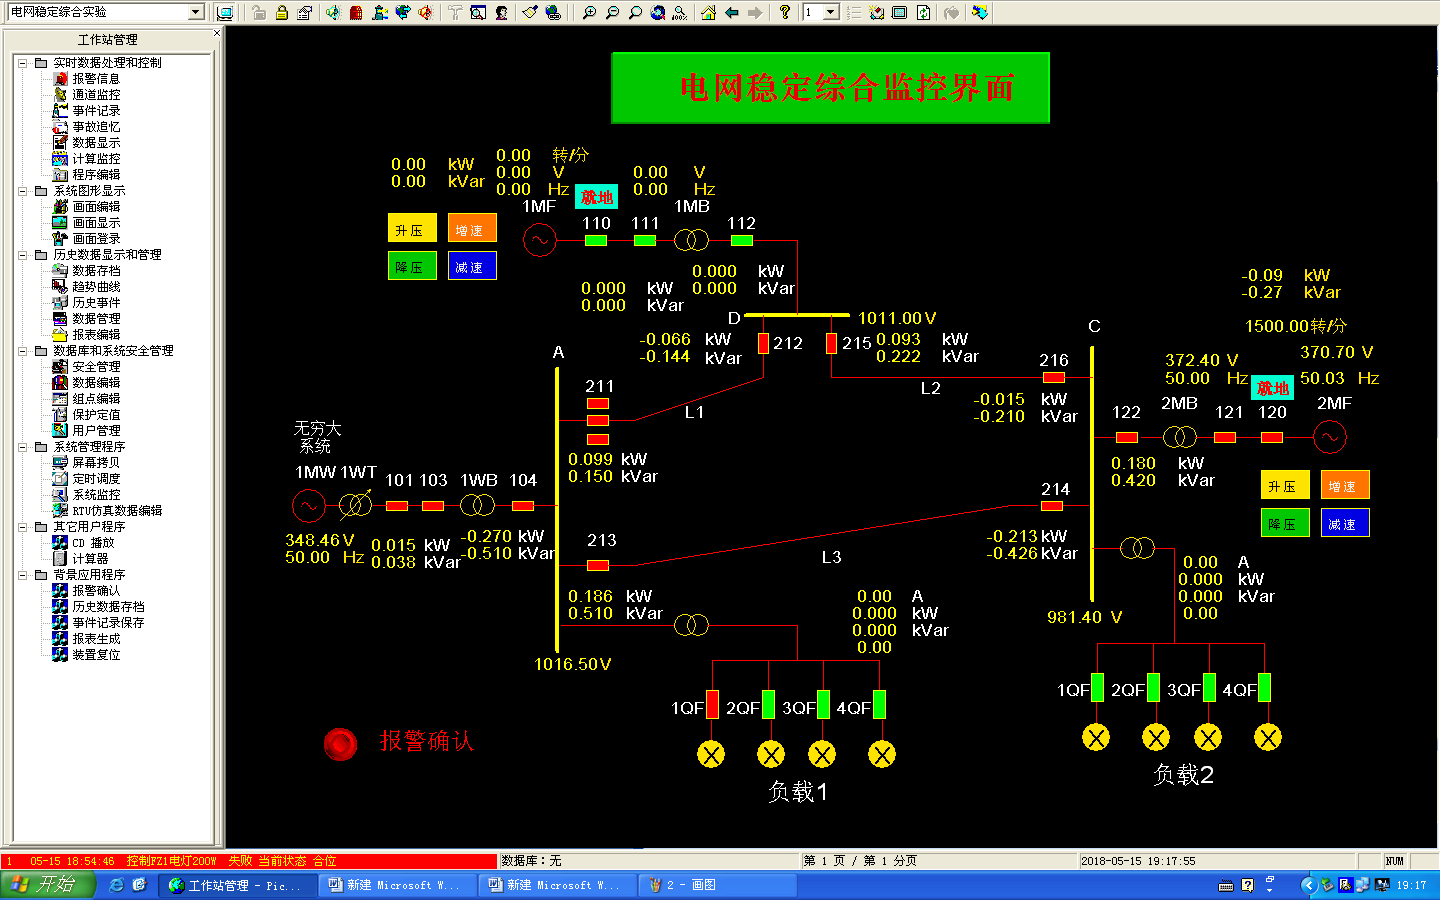
\includegraphics[width=12cm]{8.png}
                        \caption{投入负载2的容性负载前}
                    \end{figure}

                    \begin{figure}[htbp]
                        \centering
                        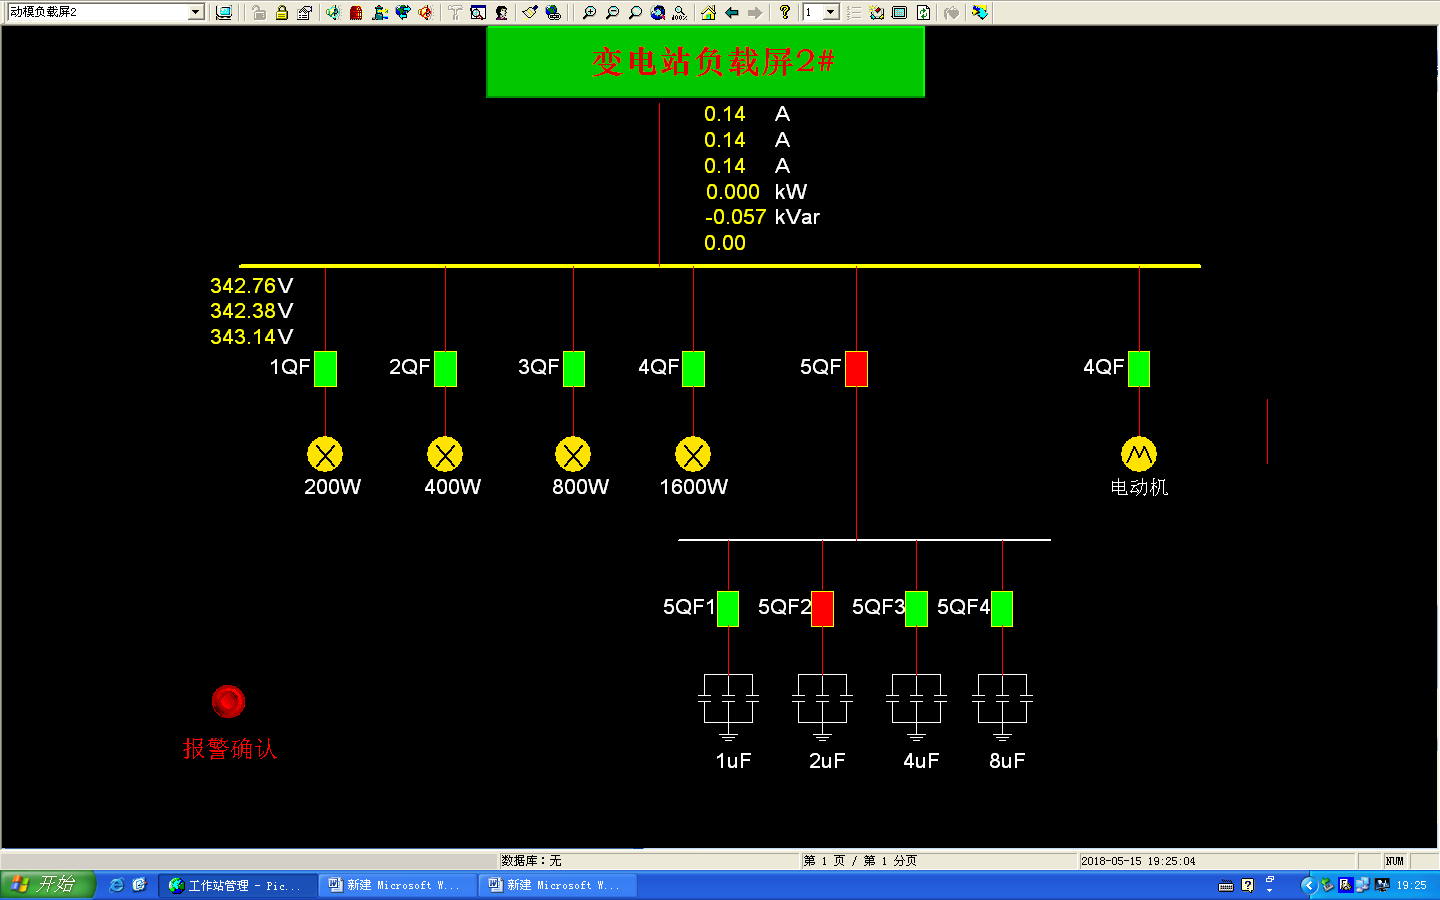
\includegraphics[width=12cm]{9.png}
                        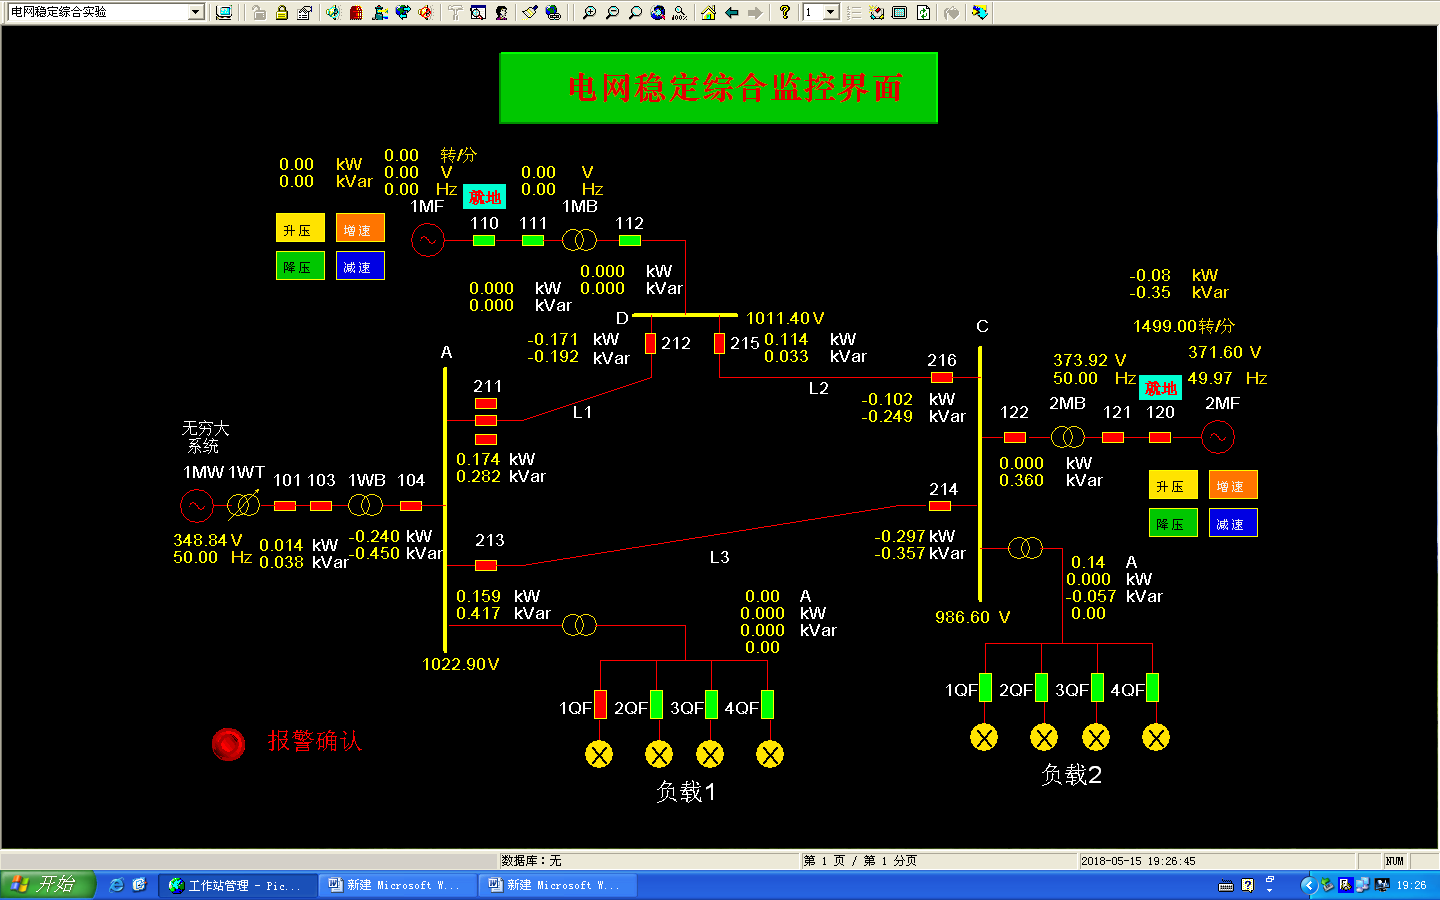
\includegraphics[width=12cm]{10.png}
                        \caption{投入负载2的$2\mu F$容性负载}
                    \end{figure}

                    \begin{table}[htbp]
                        \centering
                        \caption{投入负载2的容性负载前}
                        \centerline
                        {\begin{tabular}{|c|c|c|c|c|c|c|c|c|c|c|}
                            \hline
                            \diagbox{节点参数}{节点} & G1 & G2 & 211 & 212 & 213 & 214 & 215 & 216 & 103 & 104 \\ \hline
                            P(kW) & 0 & -0.09 & 0.372 & -0.066 & 0.186 & -0.213 & 0.093 & -0.015 & 0.015 & -0.27 \\ \hline
                            Q(kVar) & 0 & -0.27 & 0.15 & -0.144 & 0.51 & -0.426 & 0.222 & -0.21 & 0.038 & -0.51  \\ \hline
                            U(V) & 0 & 370.7 & 1016.5 & 1011 & 1016.5 & 981.4 & 1011 & 981.4 & 348.46 & 348.46 \\ \hline
                            $cos\varphi$ & 0 & -0.316 & 0.927 & -0.417 & 0.343 & -0.447 & 0.386 & -0.071 & 0.367 & -0.468 \\
                            \hline
                        \end{tabular}}
                    \end{table}

                    \begin{table}[htbp]
                        \centering
                        \caption{投入负载2的$2\mu F$容性负载}
                        \centerline
                        {\begin{tabular}{|c|c|c|c|c|c|c|c|c|c|c|}
                            \hline
                            \diagbox{节点参数}{节点} & G1 & G2 & 211 & 212 & 213 & 214 & 215 & 216 & 103 & 104 \\ \hline
                            P(kW) & 0 & -0.08 & 0.174 & -0.171 & 0.159 & -0.297 & 0.114 & -0.102 & 0.014 & -0.24 \\ \hline
                            Q(kVar) & 0 & -0.35 & 0.282 & -0.192 & 0.417 & -0.357 & 0.033 & -0.249 & 0.038 & -0.45 \\ \hline
                            U(V) & 0 & 371.6 & 1022.9 & 1011.4 & 1022.9 & 986.6 & 1011.4 & 986.6 & 348.84 & 348.84 \\ \hline
                            $cos\varphi$ & 0 & -0.223 & 0.525 & -0.665 & 0.356 & -0.64 & 0.961 & -0.379 & 0.346 & -0.471 \\
                            \hline
                        \end{tabular}}
                    \end{table}

                \newpage

                \subsection{改变网络结构的潮流分布}
                    改变网络结构不调整负载量,分别退出各线路(注意:各节点之间不能失去电气联系)。观察网络改变前后,各机组参数的变化,并记录数据于表2.8和表2.9中。

                    \begin{figure}[htbp]
                        \centering
                        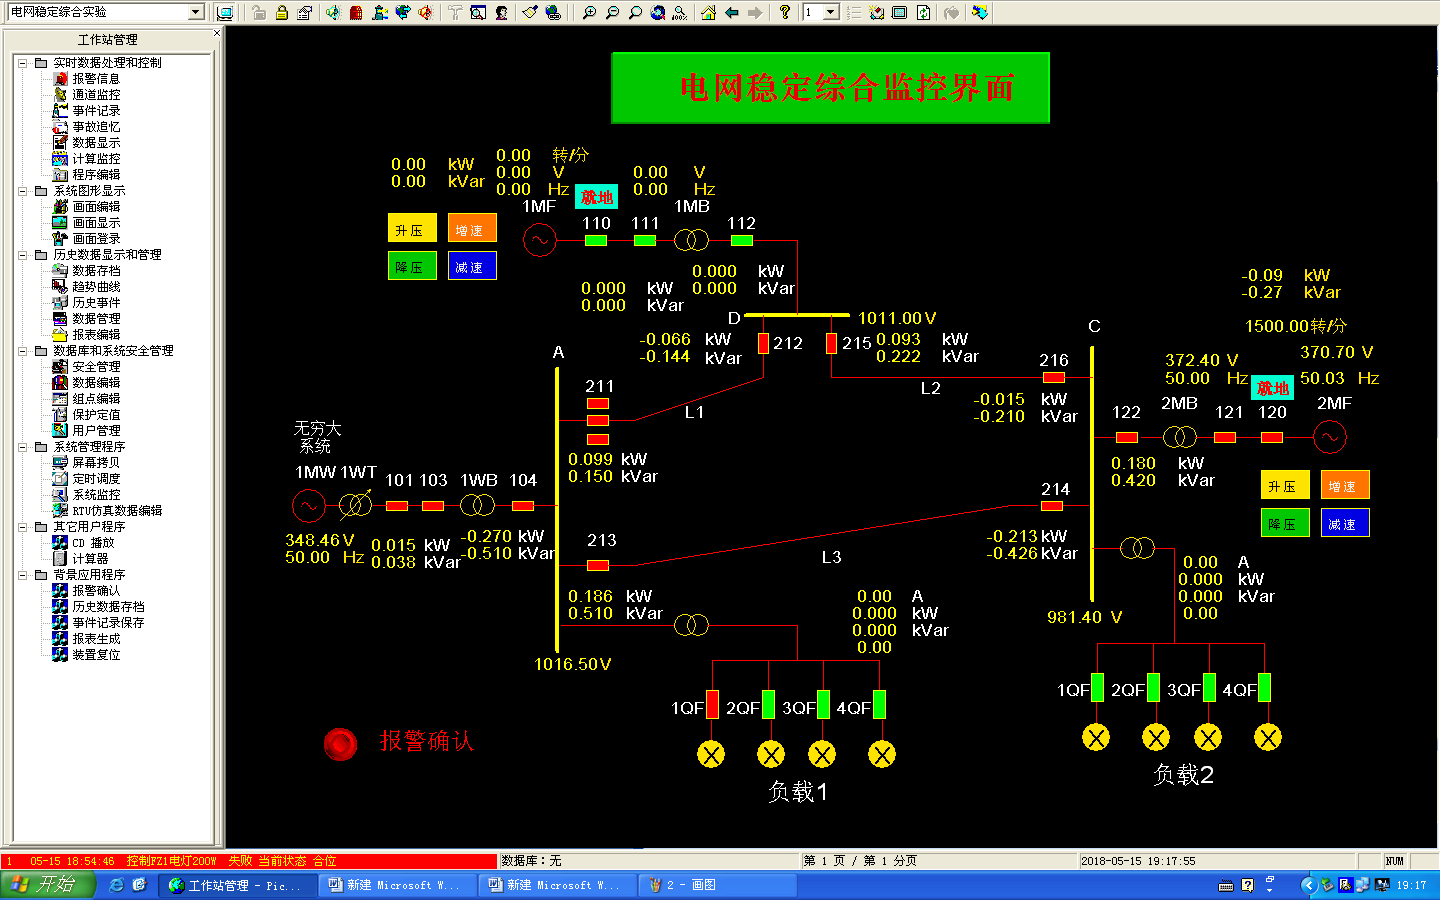
\includegraphics[width=12cm]{8.png}
                        \caption{改变网络结构前}
                    \end{figure}

                    \begin{figure}[htbp]
                        \centering
                        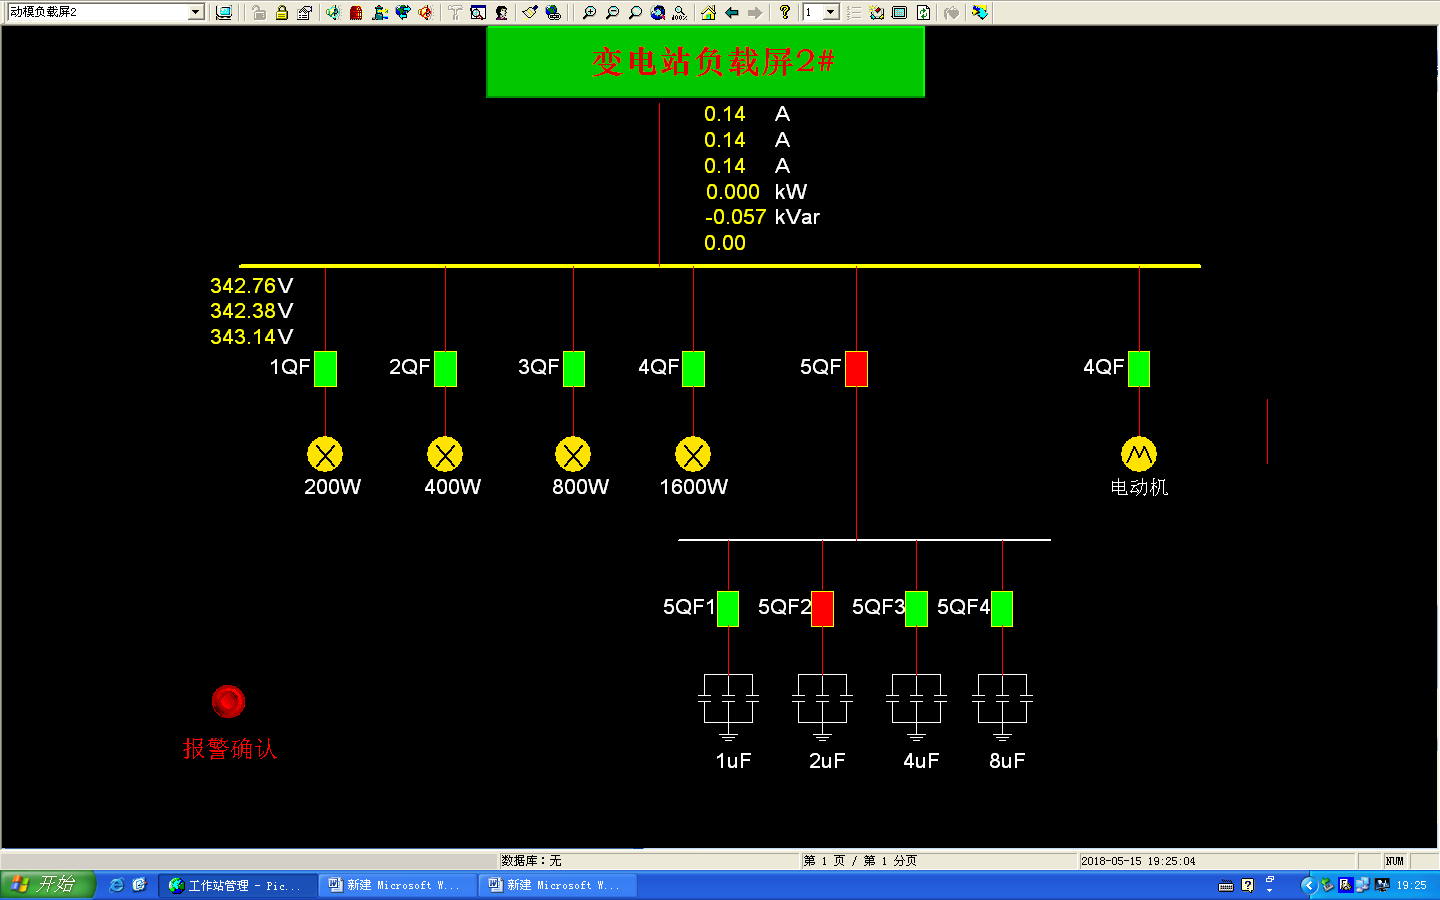
\includegraphics[width=12cm]{9.png}
                        \caption{断开断路器213后}
                    \end{figure}

                    \begin{table}[htbp]
                        \centering
                        \caption{改变网络结构前}
                        \centerline
                        {\begin{tabular}{|c|c|c|c|c|c|c|c|c|c|c|}
                            \hline
                            \diagbox{节点参数}{节点} & G1 & G2 & 211 & 212 & 213 & 214 & 215 & 216 & 103 & 104 \\ \hline
                            P(kW) & 0 & -0.08 & 0.174 & -0.171 & 0.159 &-0.297 & 0.114 & -0.102 & 0.014 & -0.24 \\ \hline
                            Q(kVar) & 0 & -0.35 & 0.282 & -0.192 & 0.417 & -0.357 & 0.033 & -0.249 & 0.038 & -0.45  \\ \hline
                            U(V) & 0 & 371.6 & 1022.9 & 1011.4 & 1022.9 & 986.6 & 1011.4 & 986.6 & 348.84 & 348.84 \\ \hline
                            $cos\varphi$ & 0 & -0.223 & 0.525 & -0.665 & 0.356 & -0.64 & 0.961 & -0.379 & 0.346 & -0.471 \\
                            \hline
                        \end{tabular}}
                    \end{table}

                    \begin{table}[htbp]
                        \centering
                        \caption{断开断路器213后}
                        \centerline
                        {\begin{tabular}{|c|c|c|c|c|c|c|c|c|c|c|}
                            \hline
                            \diagbox{节点参数}{节点} & G1 & G2 & 211 & 212 & 213 & 214 & 215 & 216 & 103 & 104 \\ \hline
                            P(kW) & 0 & -0.13 & 0.324 & -0.234 & 0.033 & 0.048 & 0.225 & -0.231 & 0.015 & -0.27 \\ \hline
                            Q(kVar) & 0 & -0.04 & 0.273 & -0.288 & 0.06 & -0.06 & 0.225 & -0.18 & 0.029 & -0.21 \\ \hline
                            U(V) & 0 & 366.8 & 999.3 & 985.9 & 999.3 & 958.9 & 985.9 & 958.9 & 348.84 & 348.84 \\ \hline
                            $cos\varphi$ & 0 & -0.956 & 0.765 & -0.631 & 0.482 & 0.625 & 0.707 & -0.789 & 0.459 & -0.789 \\
                            \hline
                        \end{tabular}}
                    \end{table}

                \newpage

                \subsection{保证系统正常运行的调度控制}
                    实验内容与实验4.2内容类似。


        \chapter{电力系统分区调频实验}
            \graphicspath{{figures_3/}}
                \section{实验目的}
                    1) 掌握区域电网调度分区调频的策略。

                    2) 掌握区域电网调度分区调频的方法。

                \section{原理与说明}
                    将几个区域电力系统相互连接起来构成的大型电力系统即联合电力系统。 联合电力系统的调频原则是:区域内部有功功率就地平衡,区域之间联络线有功功率按协议计划值传送。 
                    
                    电力系统频率和有功功率控制是调度自动化系统的一项重要任务,其主要 工作是: 
                    
                    1) 使系统的总发电出力满足系统总负荷的要求-调速控制(一次调频) 
                    
                    2) 使电力系统的运行频率和额定频率之间的误差趋于零-通过调节发电 机的频率特性实现(二次调频) 
                    
                    3) 在联合电力系统各成员之间合理分配发电出力,使联络线交换的功率满 足预先商定的计划值。

                \section{实验内容}
                    \subsection{实验系统准备}
                        本实验采用‘2MF—无穷大’系统,一次接线图如图2.1。
                    
                        利用无穷大系统屏、系统升压屏、机组、机组控屏、变压器屏、网络屏等构成电网供电系统,利用变电站低压模拟屏、负载屏、负载等构成配电系统。
                        
                        图3.1中,断路器对应顺序为:
                        
                        \begin{center}
                            \begin{tabular}{|c|c|c|c|}
                                \hline
                                断路器编号 & 对应位置 & 断路器编号 & 对应位置 \\ \hline
                                101 & 无穷大系统屏 & 122 & 变压器T2高压侧 \\ \hline
                                103 & 系统升压屏低压侧  & 211 & 网络屏1QF \\ \hline
                                104 & 系统升压屏高压侧 & 212 & 网络屏2QF \\ \hline
                                110 & 1\#机组控制屏1QF & 213 & 网络屏3QF \\ \hline
                                111 & 变压器T1低压侧 & 214 & 网络屏4QF \\ \hline
                                112 & 变压器T1高压侧 & 215 & 网络屏5QF \\ \hline
                                120 & 2\#机组控制屏1QF & 216 & 网络屏6QF \\ \hline
                                121 & 变压器T2低压侧 & & \\
                                \hline
                            \end{tabular}
                        \end{center}

                        实验接线参照图3.2
                        
                        \textbf{注意:接线前务必断开所有电源以及无穷大系统出线开关。接线完毕后务必多次检查连线是否正确,特别是相序和高低压不能出错。}

                        接线步骤如下: 
                        
                        A、接线屏上无穷大系统连接至升压变压器入端,升压变压器出端连接网络屏 1QF 入端,同时将网络屏 3QF 入端并入 1QF 入端; 
                        
                        B、1QF 出端连接至线路 L1 入端,线路 L1 出端连接至 2QF 入端,2QF 出 端连接至 5QF 入端,5QF 出端连接至线路 L2 入端,线路 L2 出端连接至 6QF 入端; 
                        
                        C、6QF 出端连接至线路 4QF 出端,3QF 出端连接至 L3 入端,L3 出端连 接至 4QF 入端,4QF 出端连接至 6QF 出端; 
                        
                        D、接线屏上机组 1 连接至变压器 T1 入端,变压器 T1 出端连接网络屏 5QF入端,同时机组 2 连接至变压器 T2 入端,变压器 T2 出端连接网络屏 4QF 出端;

                        \begin{figure}[htbp]
                            \centering
                            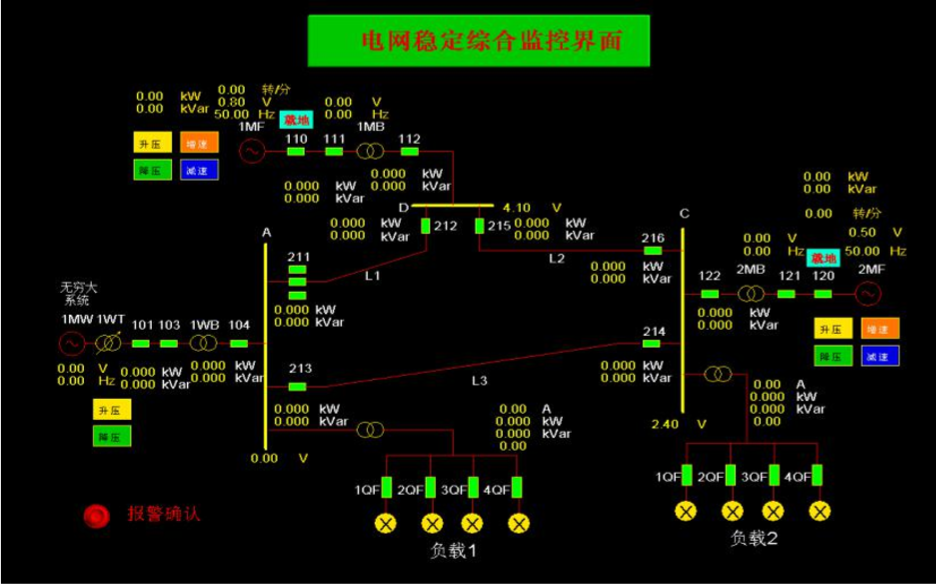
\includegraphics[width=12cm]{1.png}
                            \caption{实验供电系统一次示意图}
                        \end{figure}
        
                        \begin{figure}[htbp]
                            \centering
                            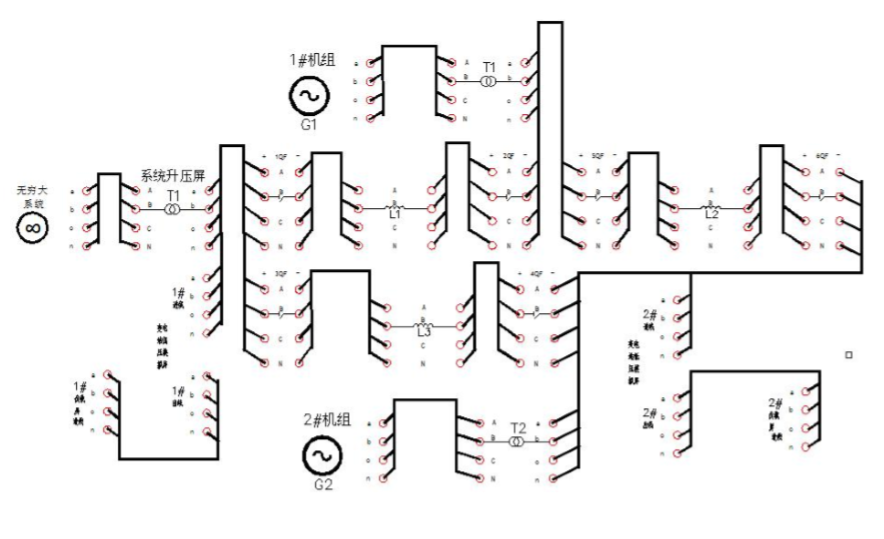
\includegraphics[width=12cm]{2.png}
                            \caption{实验供电系统一次接线图}
                        \end{figure}

                    \newpage

                    \subsection{启动主站系统}
                        要求:
                        
                        1) 完成主站系统的启动,进入“电网稳定综合监控界面”。 
                        
                        2) 记录实际的启动步骤,以及观察到的界面。
                        
                        3) 主站系统启动步骤参考如下: 
                        
                        4) 双击桌面上的“启动 Centra2000”图标出现 Centra2000 的工作站管理 界面。
                        
                        5) 点击屏幕左上方的“锁”后,弹出系统登录对话框。选择操作员类型, 输入口令,进入系统主界面。
                        
                        6) 点击屏幕左上方的“显示器”后,打开工作站管理的程序列表。 
                        
                        7) 工作站管理界面由工具栏、程序列表和图像操作窗口组成。 
                        
                        8) 在系统主界面中,有11个按钮,分别为:发电机1\#、发电机2\#、高压屏、低压屏、负载屏1\#、负载屏2\#、网络屏、无穷大系统站、电网稳定综合监控、变电站综合监控和分区调频监控,点击进入“电网稳定综合监控界面”。

                    \subsection{实验系统运行方式准备}
                        \noindent 1.要求
                        
                        1) 通过遥控操作,将实验系统的运行方式调整为:退出无穷大系统;电网视为两个区域,1\#发电机通过线路 L1、母线 A 向负载 1 供电,为区域 A;2\#发电机通过母线 C 向负载 2 供电,为区域 B;线路 L2 为区域 A 和 B 之间的联络线。
                       
                        2) 记录实际的操作步骤,以及观察到的界面和运行参数。
                        
                        \noindent 2.操作内容
                        
                        1)遥控退出所有负荷,调整发电机出力和励磁,使频率、发电机端电压满足要求。
                       
                        2)遥控断开 213、214 节点。数据参数见表3.1

                        3)遥控断开 104节点。数据参数见表3.2

                        4)此时,电网视为两个区域,1\#发电机通过线路 L1、母线 A 向负载 1 供电,为区域 A;2\#发电机通过母线 C 向负载 2 供电,为区域 B;线路 L2 为区域A 和 B 之间的联络线。

                        \begin{figure}[htbp]
                            \centering
                            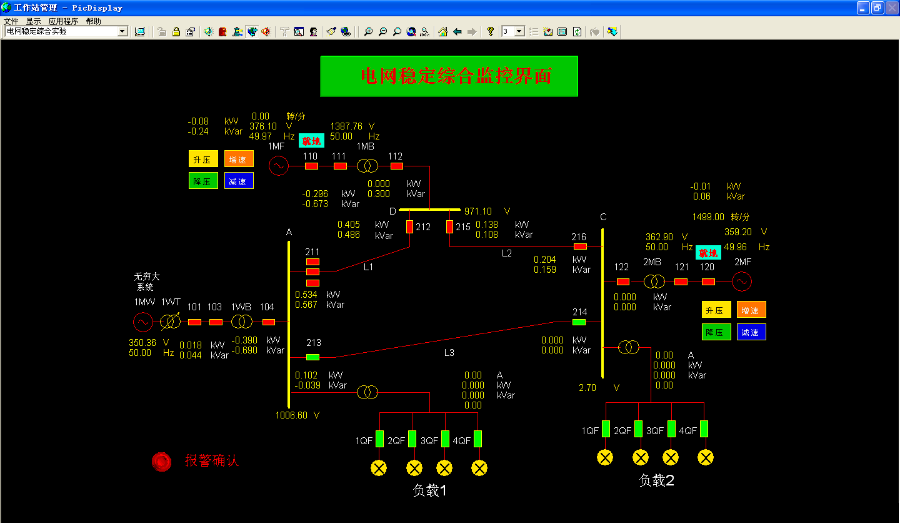
\includegraphics[width=12cm]{3.png}
                            \caption{遥控断开 213、214 节点}
                        \end{figure}

                        \begin{table}[htbp]
                            \centering
                            \caption{遥控断开 213、214 节点}
                            \centerline
                            {\begin{tabular}{|c|c|c|c|c|c|c|c|c|c|}
                                \hline
                                \diagbox{节点参数}{节点} & G1 & G2 & S无穷大 & 211 & 212 & 213 & 214 & 215 & 216 \\ \hline
                                P(kW) & -0.08 & 0.01 & / & 0.534 & 0.405 & 0.102 & 0 & 0.138 & 0.204 \\ \hline
                                Q(kVar) & -0.24 & 0.06 & / & 0.587 & 0.486 & -0.039 & 0 & 0.108 & 0.159 \\ \hline
                                U(V) & 376.1 & 359.2 & 350.36 & 1006.6 & 971.1 & 1006.6 & 2.7 & 971.1 & 2.7 \\ \hline
                                $cos\varphi$ & -0.316 & 0.164 & / & 0.673 & 0.640 & 0.934 & / & 0.788 & 0.789 \\
                                \hline
                            \end{tabular}}
                        \end{table}

                        \begin{figure}[htbp]
                            \centering
                            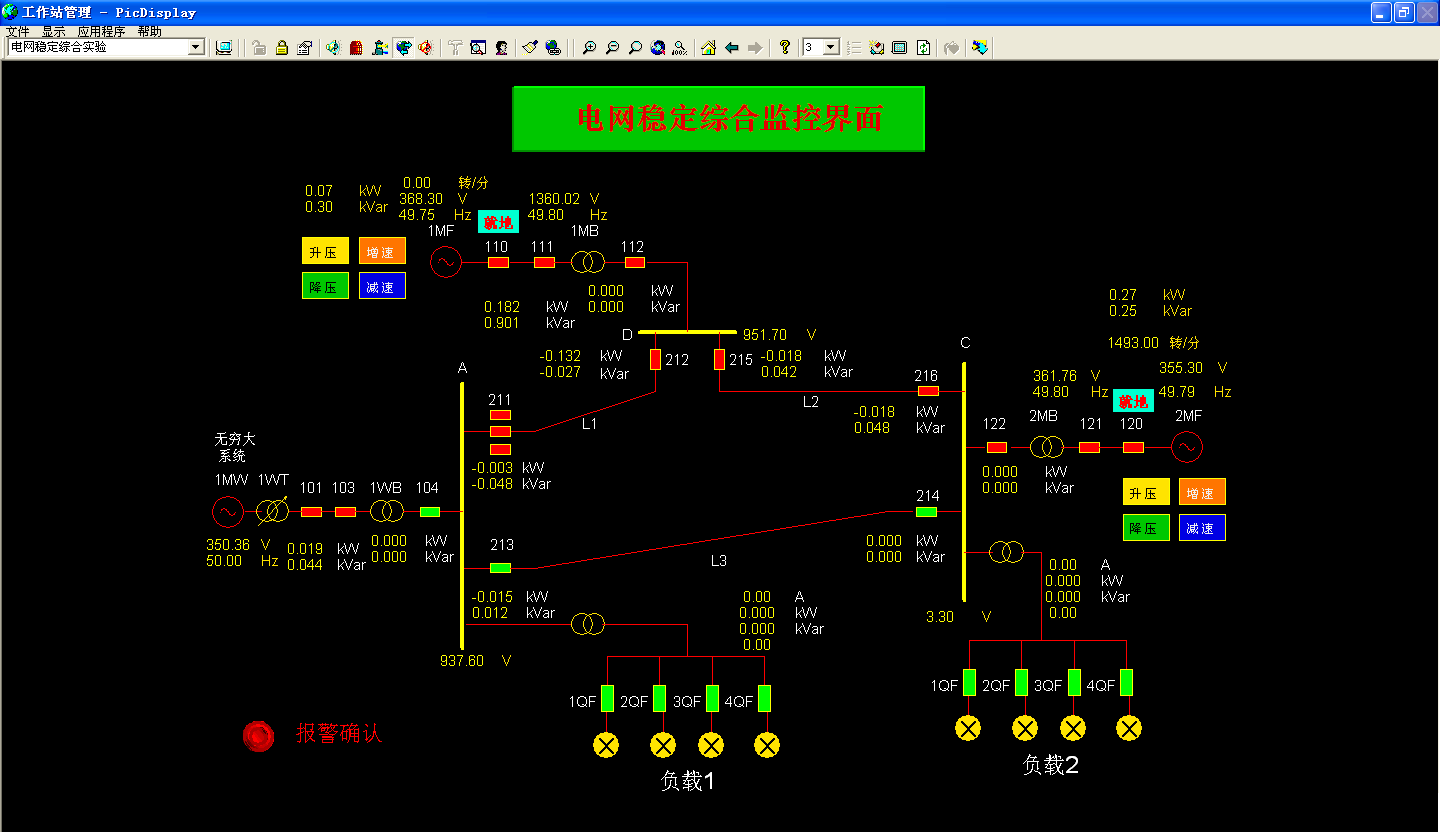
\includegraphics[width=12cm]{4.png}
                            \caption{遥控断开 104节点}
                        \end{figure}

                        \begin{table}[htbp]
                            \centering
                            \caption{遥控断开 104节点}
                            \centerline
                            {\begin{tabular}{|c|c|c|c|c|c|c|c|c|c|}
                                \hline
                                \diagbox{节点参数}{节点} & G1 & G2 & S无穷大 & 211 & 212 & 213 & 214 & 215 & 216 \\ \hline
                                P(kW) & 0.07 & 0.27 & / & -0.003 & -0.132 & -0.015 & 0 & -0.018 & -0.018  \\ \hline
                                Q(kVar) & 0.3 & 0.25 & / & -0.048 & -0.027 & 0.012 & 0 & 0.042 & 0.048 \\ \hline
                                U(V) & 368.3 & 355.3 & 350.36 & 937.6 & 951.7 & 937.6 & 3.3 & 951.7 & 3.3 \\ \hline
                                $cos\varphi$ & 0.227 & 0.734 & / & -0.0624 & -0.98 & -0.781 & / & -0.394 & -0.351 \\
                                \hline
                            \end{tabular}}
                        \end{table}

                    \newpage

                    \subsection{$\Delta P_{AB}=0$时分区调频}
                        \noindent 1.要求
                        
                        1) 改变负荷大小,通过遥控遥调操作,满足协议交换功率为 0 的要求,即$\Delta P_{AB}=0$,两个区域之间无有功功率交换。
                        
                        2) 记录实际的操作步骤,以及观察到的界面和运行参数。 
                        
                        3) 对调频原理、过程及结果进行分析。
                        
                        \noindent 2.操作内容
                        
                        1)由于目的是使得$\Delta P_{AB}=0$,因此需要增加功率输出,所以首先改变发电机转速,即调整发电机功率输出,观察联络线上212与215功率能否得到结果。
                        对发电机2进行增速操作,结果数据见表3.3

                        \begin{figure}[htbp]
                            \centering
                            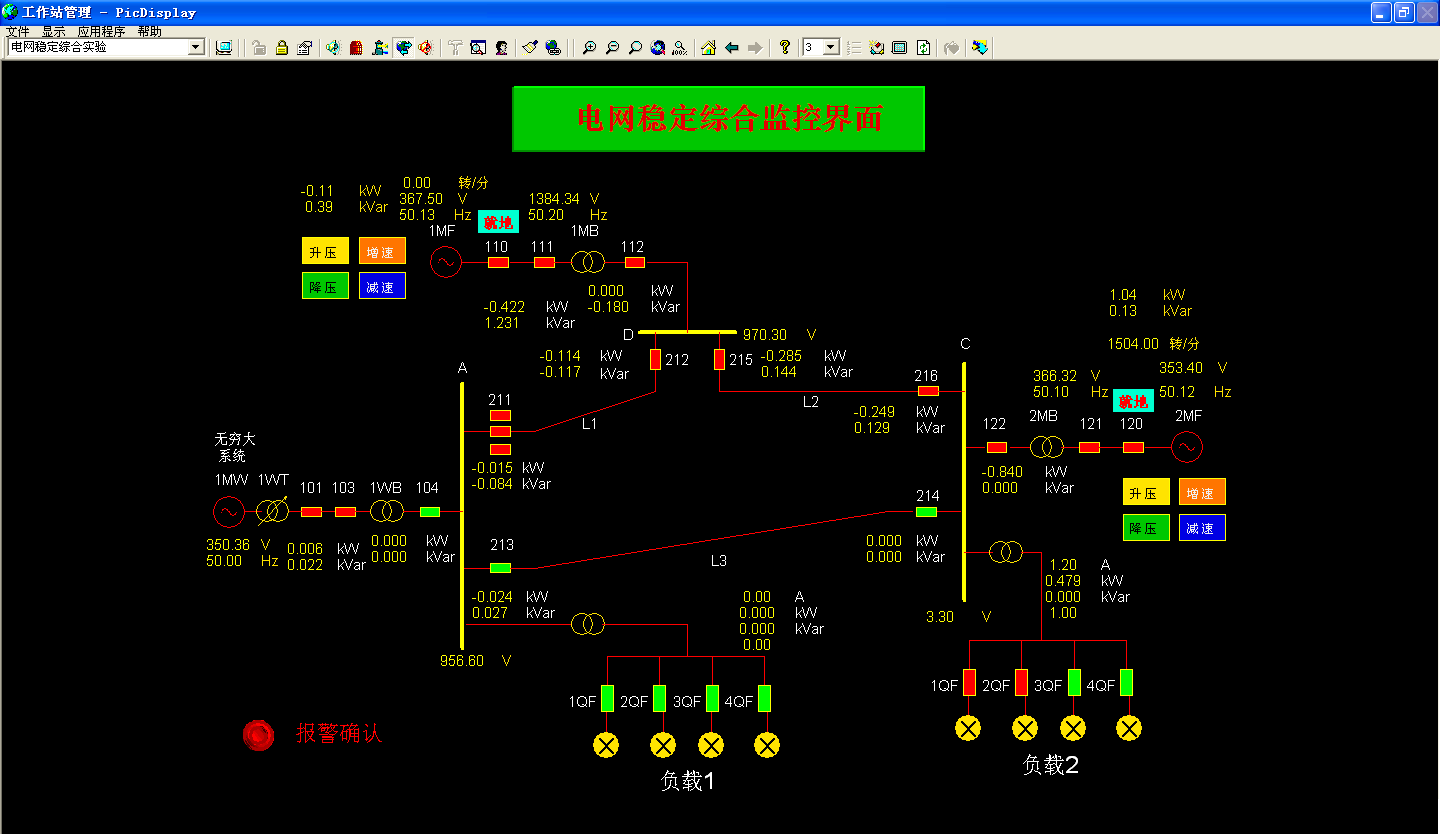
\includegraphics[width=12cm]{5.png}
                            \caption{发电机2增速}
                        \end{figure}

                        \begin{table}[htbp]
                            \centering
                            \caption{发电机2增速}
                            \centerline
                            {\begin{tabular}{|c|c|c|c|c|c|c|c|c|c|}
                                \hline
                                \diagbox{节点参数}{节点} & G1 & G2 & S无穷大 & 211 & 212 & 213 & 214 & 215 & 216 \\ \hline
                                P(kW) & -0.01 & 0.92 & / & -0.216 & -0.066 & -0.075 & 0 & -0.03 & -0.069 \\ \hline
                                Q(kVar) & 0.37 & 0.17 & / & -0.093 & -0.210 & -0.102 & 0 & 0.102 & 0.082  \\ \hline
                                U(V) & 367.3 & 353.8 & 350.36 & 953.7 & 970.7 & 953.7 & 0.9 & 970.7 & 0.9 \\ \hline
                                $cos\varphi$ & -0.027 & 0.98 & / & -0.918 & -0.3 & -0.592 & / & -0.282 & -0.648 \\
                                \hline
                            \end{tabular}}
                        \end{table}

                        \newpage

                        2)改变负载,并调节发电机频率观察212与215交换功率是否为0。合上负载1中QF3与QF4,结果数据见表3.4。由于没有达到要求,故再次对发电机进行增速调节使其满足要求。

                        \begin{figure}[htbp]
                            \centering
                            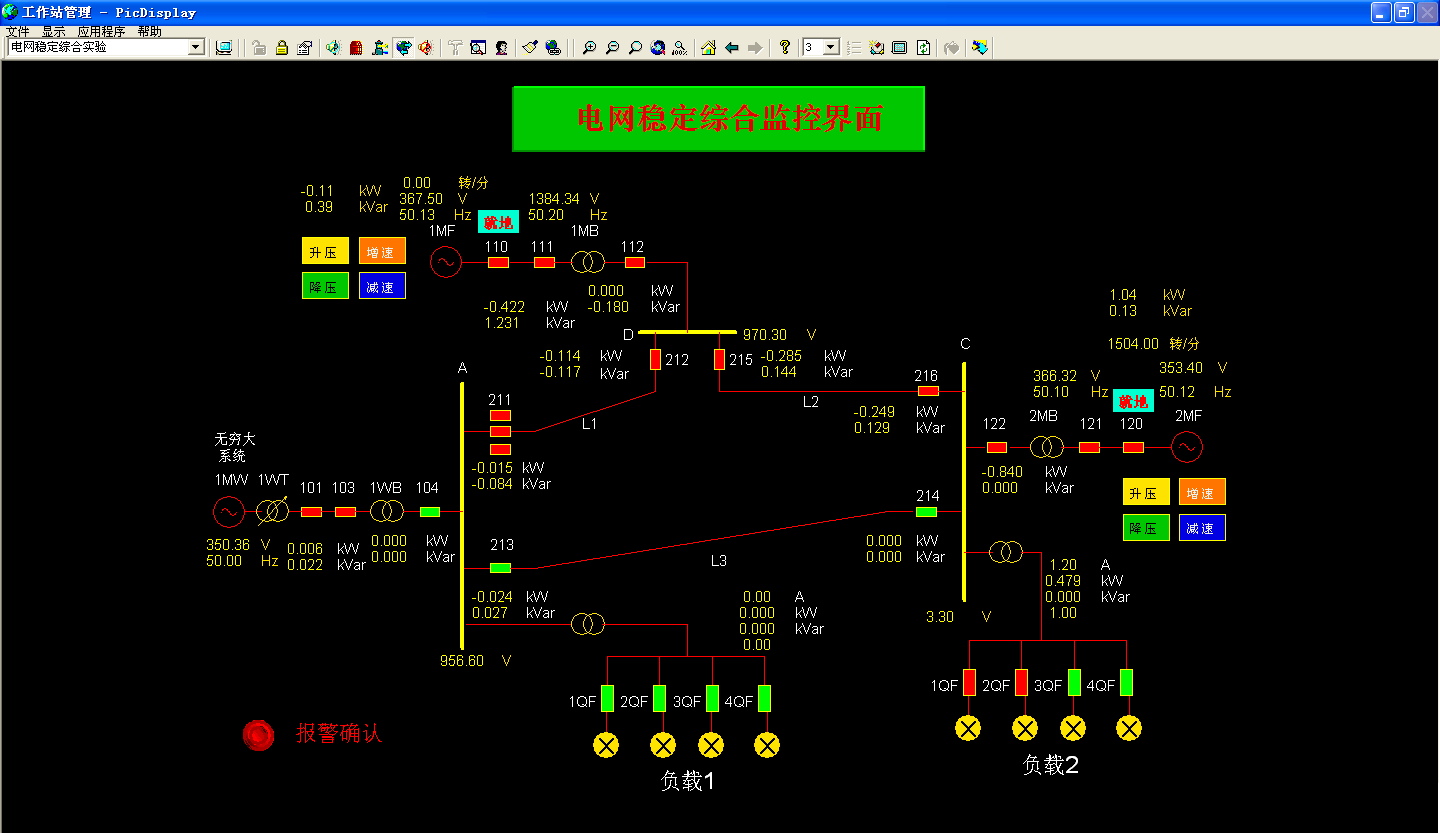
\includegraphics[width=12cm]{6.png}
                            \caption{合上负载1中QF3与QF4}
                        \end{figure}

                        \begin{table}[htbp]
                            \centering
                            \caption{合上负载1中QF3与QF4}
                            \centerline
                            {\begin{tabular}{|c|c|c|c|c|c|c|c|c|c|}
                                \hline
                                \diagbox{节点参数}{节点} & G1 & G2 & S无穷大 & 211 & 212 & 213 & 214 & 215 & 216 \\ \hline
                                P(kW) & 0.09 & 1.42 & / & -0.702 & -0.683 & -0.039 & 0 & -0.687 & -0.615 \\ \hline
                                Q(kVar) & 0.45 & 0.13 & / & -0.084 & -0.093 & 0 & 0 & 0.180 & 0.210 \\ \hline
                                U(V) & 366 & 352.7 & 350.36 & 938.6 & 959.5 & 938.6 & 2.1 & 959.5 & 2.1 \\ \hline
                                $cos\varphi$ & 0.196 & 0.996 & / & -0.993 & -0.991 & -1 & / & -0.967 & -0.946 \\
                                \hline
                            \end{tabular}}
                        \end{table}
                       
                        3)将观察线路转移至213与214线路,再次改变负载与发电机转速,观察交换功率是否为0。
                        
                        合上节点213与214,并合上104节点,将无穷大系统接入系统,然后断开节点215、216,并断开112节点,将发电机G1移除系统。断开节点211。将负载3QF与4QF断开。此时A、B区域间仅由L3连接,即观察节点213与214间交换功率是否得0。结果数据见表3.5

                        \begin{figure}[htbp]
                            \centering
                            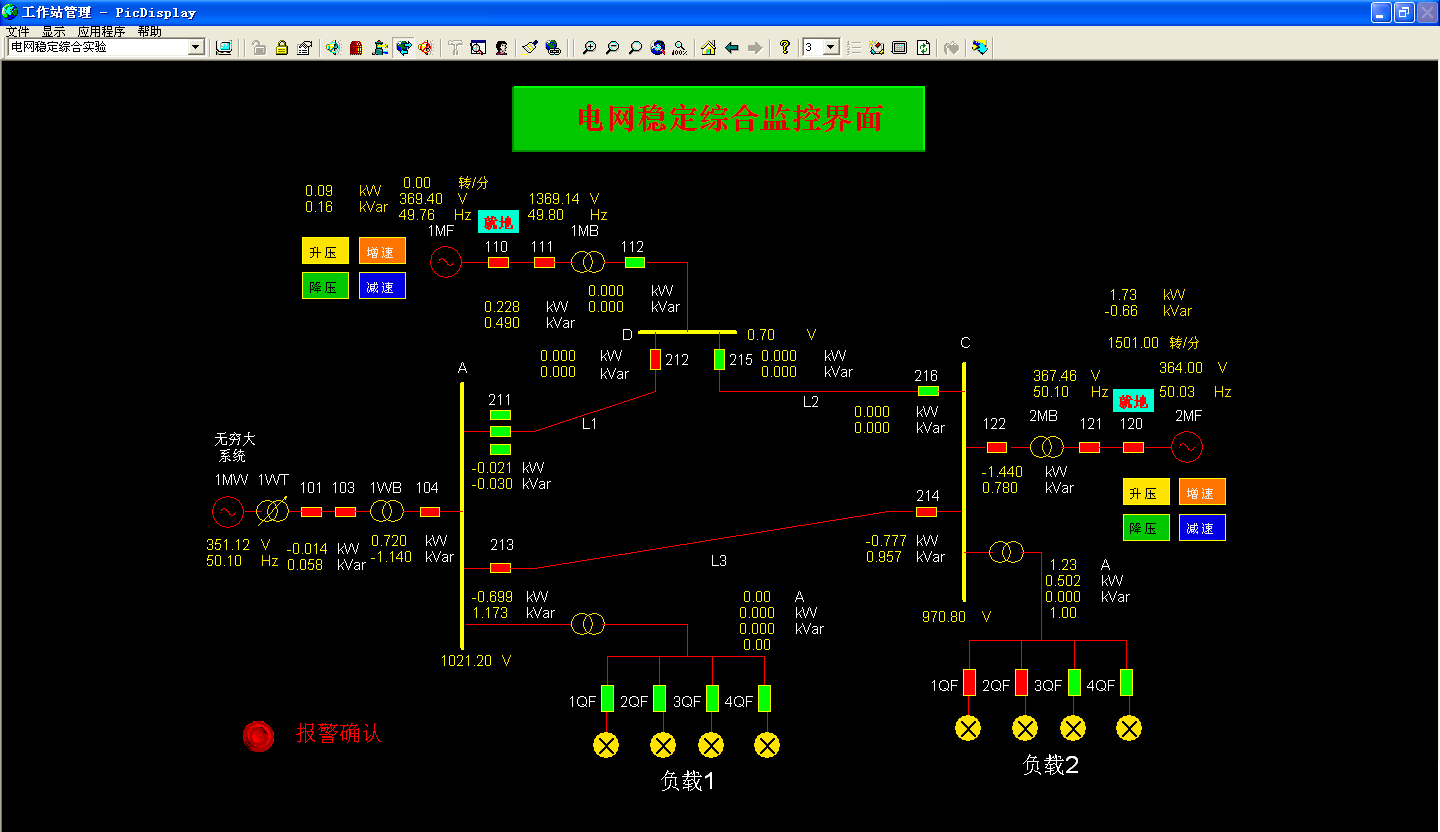
\includegraphics[width=12cm]{7.png}
                            \caption{断开L1、L2,连接L3}
                        \end{figure}

                        \begin{table}[htbp]
                            \centering
                            \caption{断开L1、L2,连接L3}
                            \centerline
                            {\begin{tabular}{|c|c|c|c|c|c|c|c|c|c|}
                                \hline
                                \diagbox{节点参数}{节点} & G1 & G2 & S无穷大 & 211 & 212 & 213 & 214 & 215 & 216 \\ \hline
                                P(kW) & 0.009 & 1.73 & -0.014 & -0.021 & 0 & -0.698 & -0.777 & 0 & 0 \\ \hline
                                Q(kVar) & 0.18 & -0.66 & 0.058 & -0.03 & 0 & 1.173 & 0.957 & 0 & 0 \\ \hline
                                U(V) & 369.4 & 354 & 351.12 & 1021.2 & 0.7 & 1021.2 & 970.8 & 0.7 & 970.8 \\ \hline
                                $cos\varphi$ & 0.050 & 0.934 & -0.234 & -0.573 & / & -0.511 & -0.63 & / & / \\
                                \hline
                            \end{tabular}}
                        \end{table}
                        
                        4)增加负载,调节发电机G2转速,观察线路L3交换功率是否为0。合上负载1中1QF与2QF,调节发电机G2转速。结果数据见表3.6

                        \begin{figure}[htbp]
                            \centering
                            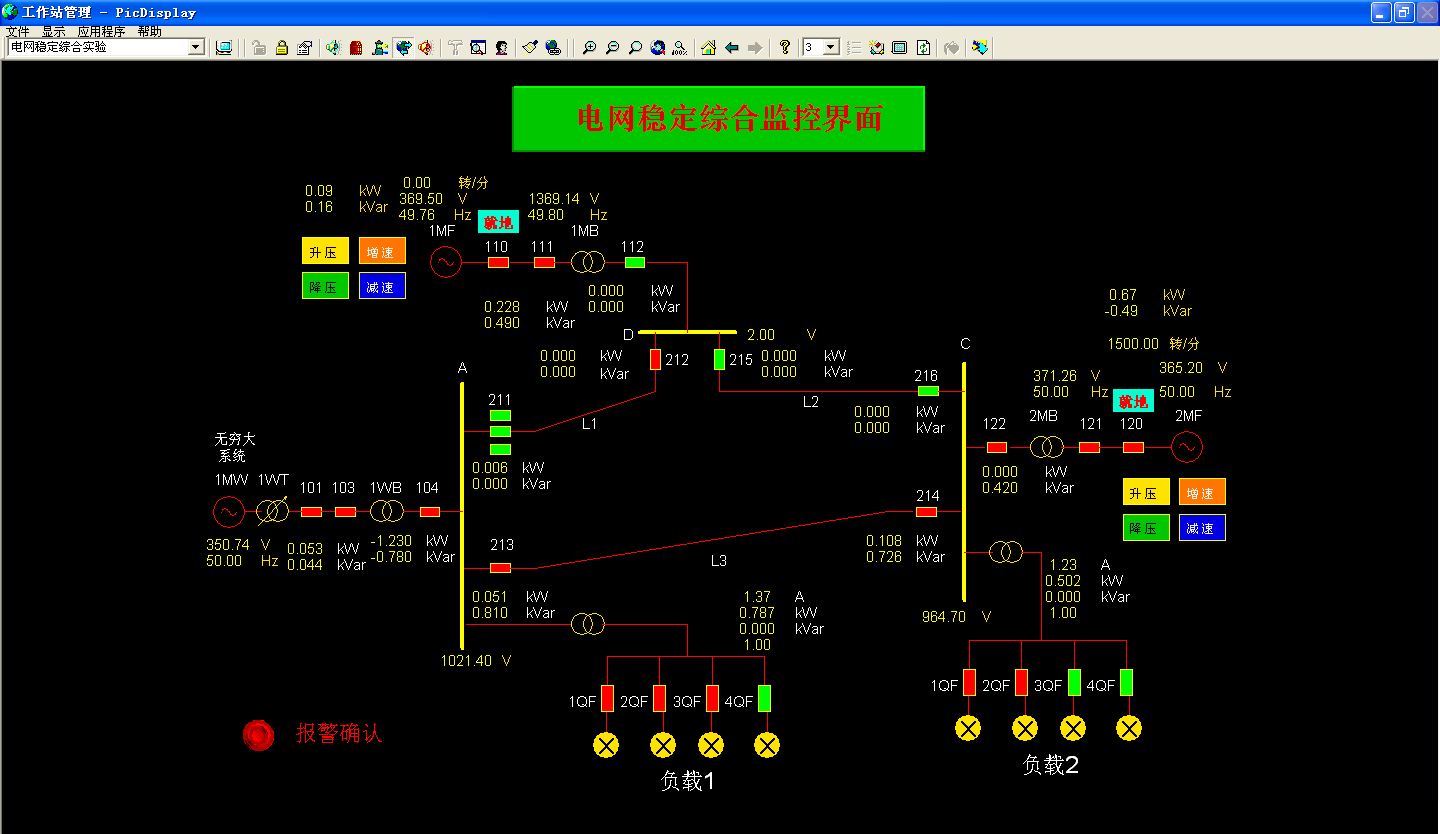
\includegraphics[width=12cm]{8.png}
                            \caption{增加负载,调节发电机G2转速}
                        \end{figure}

                        \begin{table}[htbp]
                            \centering
                            \caption{增加负载,调节发电机G2转速}
                            \centerline
                            {\begin{tabular}{|c|c|c|c|c|c|c|c|c|c|}
                                \hline
                                \diagbox{节点参数}{节点} & G1 & G2 & S无穷大 & 211 & 212 & 213 & 214 & 215 & 216 \\ \hline
                                P(kW) & 0.009 & 0.67 & 0.053 & 0.006 & 0 & 0.051 & 0.108 & 0 & 0 \\ \hline
                                Q(kVar) & 0.18 & -0.49 & 0.044 & 0 & 0 & 0.810 & 0.726 & 0 & 0 \\ \hline
                                U(V) & 369.4 & 365.2 & 350.74 & 1021.4 & 0.7 & 1021.4 & 964.7 & 0.7 & 970.8 \\ \hline
                                $cos\varphi$ & 0.050 & 0.807 & 0.769 & / & / & 0.063 & 0.147 & / & / \\
                                \hline
                            \end{tabular}}
                        \end{table}

                    \subsection{$\Delta P=1KW$时分区调频}
                        \noindent 1.要求 
                       
                        1) 改变负荷大小,通过遥控遥调操作,满足协议交换功率 A 区向 B 区输送1kW 有功功率的要求,即$\Delta P=1KW$ 。
                       
                        2) 记录实际的操作步骤,以及观察到的界面和运行参数。 
                        
                        3) 对调频原理、过程及结果进行分析
                        
                        \noindent 2.操作内容
                        
                        1)根据实验要求可知,要使得$\Delta P=1KW$,需要减少功率,因此,在3.4实验基础上先减少有功负载,观察线路L3潮流分布。断开负载2,结果数据见表3.7

                        \begin{figure}[htbp]
                            \centering
                            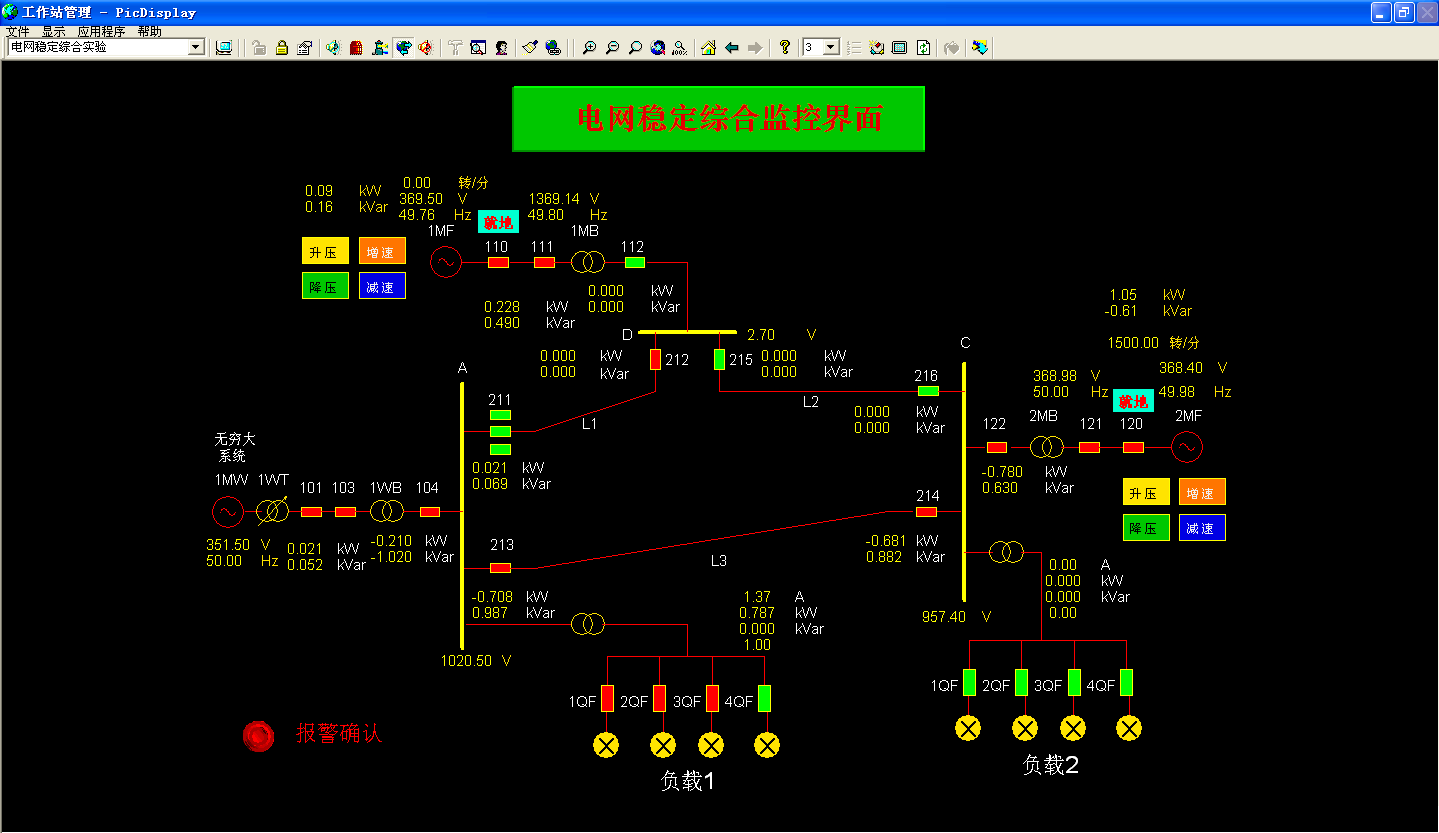
\includegraphics[width=12cm]{9.png}
                            \caption{断开负载2}
                        \end{figure}
                        
                        \begin{table}[htbp]
                            \centering
                            \caption{断开负载2}
                            \centerline
                            {\begin{tabular}{|c|c|c|c|c|c|c|c|c|c|}
                                \hline
                                \diagbox{节点参数}{节点} & G1 & G2 & S无穷大 & 211 & 212 & 213 & 214 & 215 & 216 \\ \hline
                                P(kW) & 0.009 & 0.05 & 0.021 & 0.021 & 0 & -0.708 & -0.681 & 0 & 0 \\ \hline
                                Q(kVar) & 0.18 & -0.61 & 0.052 & 0.069 & 0 & 0.987 & 0.882 & 0 & 0 \\ \hline
                                U(V) & 369.4 & 368.4 & 351.5 & 1020.5 & 2.7 & 1020.5 & 957.4 & 2.7 & 957.4 \\ \hline
                                $cos\varphi$ & 0.050 & 0.0817 & 0.374 & 0.291 & / & -0.583 & -0.611 & / & / \\
                                \hline
                            \end{tabular}}
                        \end{table}

                        \newpage

                        2)断开负载1中2QF与3QF,调节发电机转速,结果数据见表3.8

                        \begin{figure}[htbp]
                            \centering
                            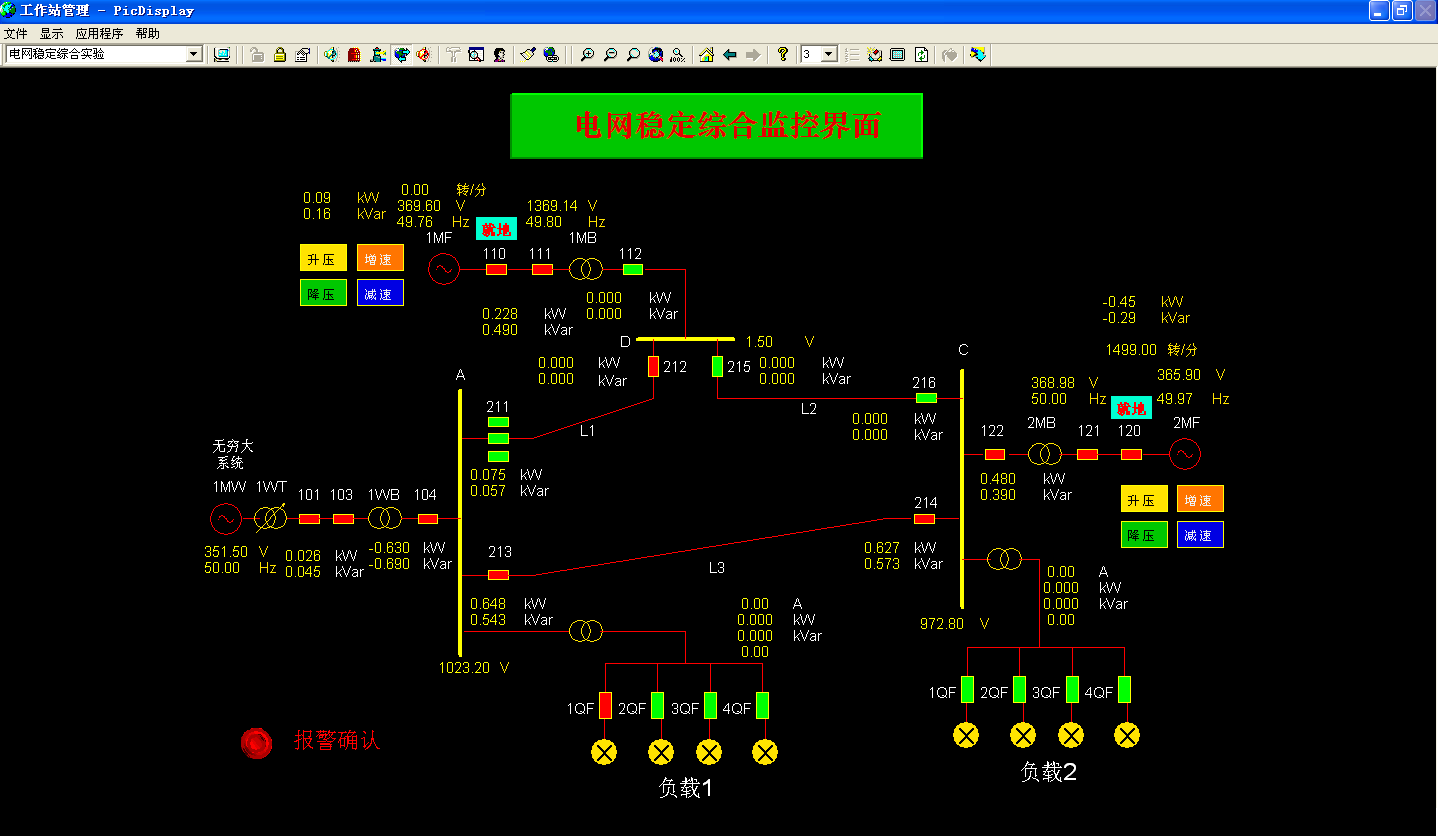
\includegraphics[width=12cm]{10.png}
                            \caption{断开负载1中2QF与3QF,调节发电机转速}
                        \end{figure}
                        
                        \begin{table}[htbp]
                            \centering
                            \caption{断开负载1中2QF与3QF,调节发电机转速}
                            \centerline
                            {\begin{tabular}{|c|c|c|c|c|c|c|c|c|c|}
                                \hline
                                \diagbox{节点参数}{节点} & G1 & G2 & S无穷大 & 211 & 212 & 213 & 214 & 215 & 216 \\ \hline
                                P(kW) & 0.009 & -0.46 & 0.026 & 0.075 & 0 & 0.648 & 0.627 & 0 & 0 \\ \hline
                                Q(kVar) & 0.18 & -0.29 & 0.045 & 0.057 & 0 & 0.543 & 0.573 & 0 & 0 \\ \hline
                                U(V) & 369.4 & 365.9 & 351.5 & 1023.2 & 1.5 & 1023.2 & 972.8 & 1.5 & 972.8 \\ \hline
                                $cos\varphi$ & 0.050 & -0.846 & 0.5 & 0.796 & / & 0.766 & 0.738 & / & / \\
                                \hline
                            \end{tabular}}
                        \end{table}

                        \newpage

                        3)增加负载2端负荷,调节发电机转速。合负载2中1QF,调节发电机转速。结果数据见表3.9

                        \begin{figure}[htbp]
                            \centering
                            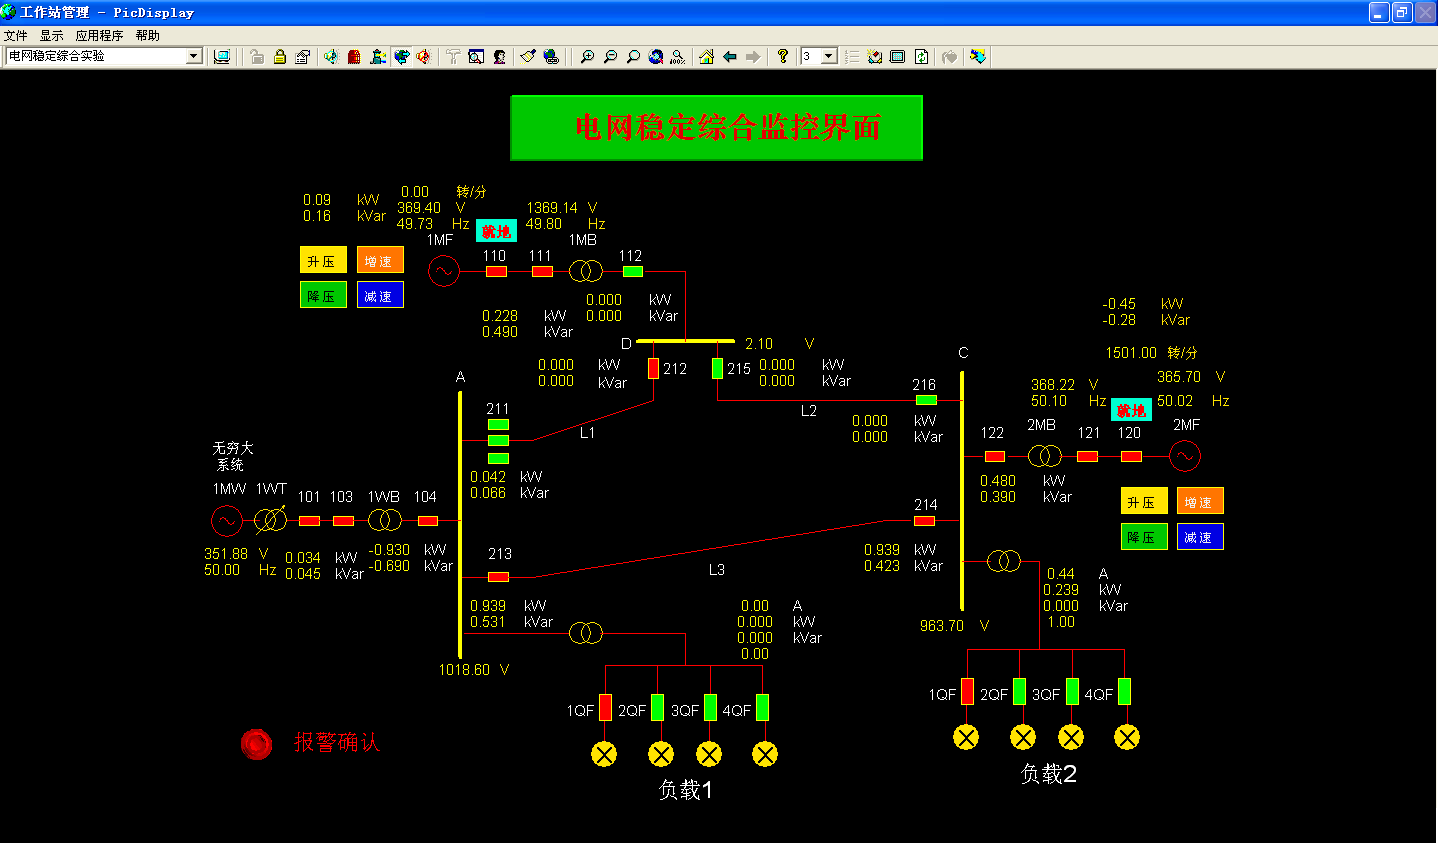
\includegraphics[width=12cm]{11.png}
                            \caption{增加负荷,调节发电机转速}
                        \end{figure}
                        
                        \begin{table}[htbp]
                            \centering
                            \caption{增加负荷,调节发电机转速}
                            \centerline
                            {\begin{tabular}{|c|c|c|c|c|c|c|c|c|c|}
                                \hline
                                \diagbox{节点参数}{节点} & G1 & G2 & S无穷大 & 211 & 212 & 213 & 214 & 215 & 216 \\ \hline
                                P(kW) & 0.009 & -0.45 & 0.034 & 0.042 & 0 & 0.939 & 0.939 & 0 & 0 \\ \hline
                                Q(kVar) & 0.18 & -0.28 & 0.045 & 0.066 & 0 & 0.531 & 0.423 & 0 & 0 \\ \hline
                                U(V) & 369.4 & 365.7 & 351.88 & 1018.8 & 2.1 & 1018.8 & 963.7 & 2.1 & 963.7 \\ \hline
                                $cos\varphi$ & 0.050 & -0.849 & 0.603 & 0.537 & / & 0.870 & 0.912 & / & / \\
                                \hline
                            \end{tabular}}
                        \end{table}

                        
   
        \chapter{能量管理的实时运行分析}
            \graphicspath{{figures_4/}} 
            \section{实验目的}
                1) 掌握能量管理的实时运行分析功能在调度自动化系统中的作用:电网实
                时运行分析是在电网实时运行情况下,利用采集到的厂站运行状态的
                实时信息,对电网运行的安全性和经济性进行分析与计算,为调度运
                行人员提供运行优化决策的依据;

                2) 了解电网实时运行分析的功能模块;

                3) 了解电网实时运行分析的实现方式。

            \section{系统结构}
                1) 能量管理的电网实时运行分析包括:

                \quad (1) 计算部分:

                \qquad a.电网的状态估计(在线潮流)

                \qquad b.电网的安全分析

                \qquad c.无功-电压的优化调度

                \quad (2) 统计部分:

                \qquad a.各厂站的负荷曲线

                \qquad b.各中枢点的电压曲线

                \qquad c.有关运行参数的统计查询

                2) 电网结构

                本系统为一 3 个发电厂、5 个变电站的 110kV 的电网。为了便于掌握分析
                和计算方法,将整个电网分为两部分:

                \quad (1) 内部系统

                \quad (2) 外部系统

                \begin{figure}[htbp]
                    \centering
                    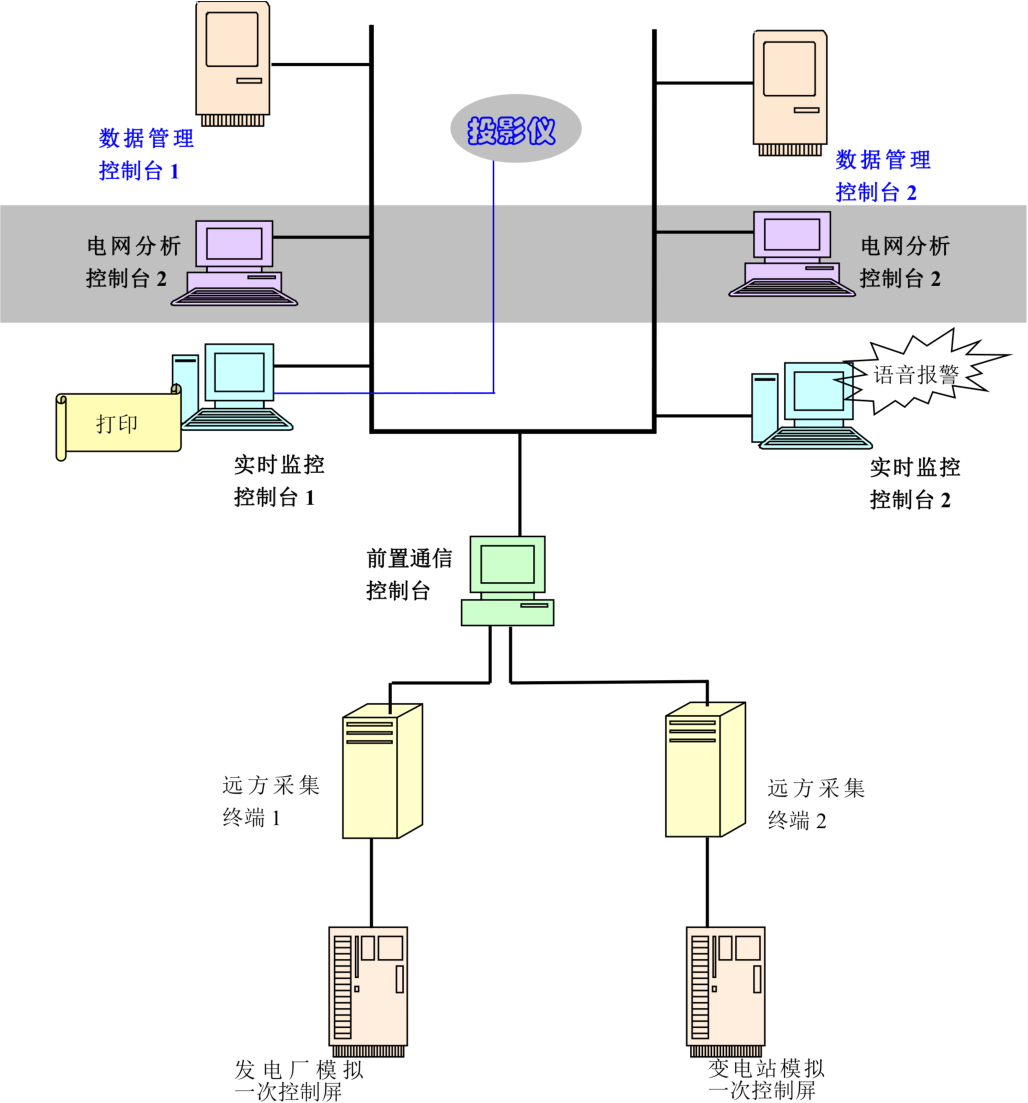
\includegraphics[width=14cm]{1.pdf}
                    \caption{系统结构}
                \end{figure}
            
            \newpage

            \section{系统功能}
                \begin{figure}[htbp]
                    \centering
                    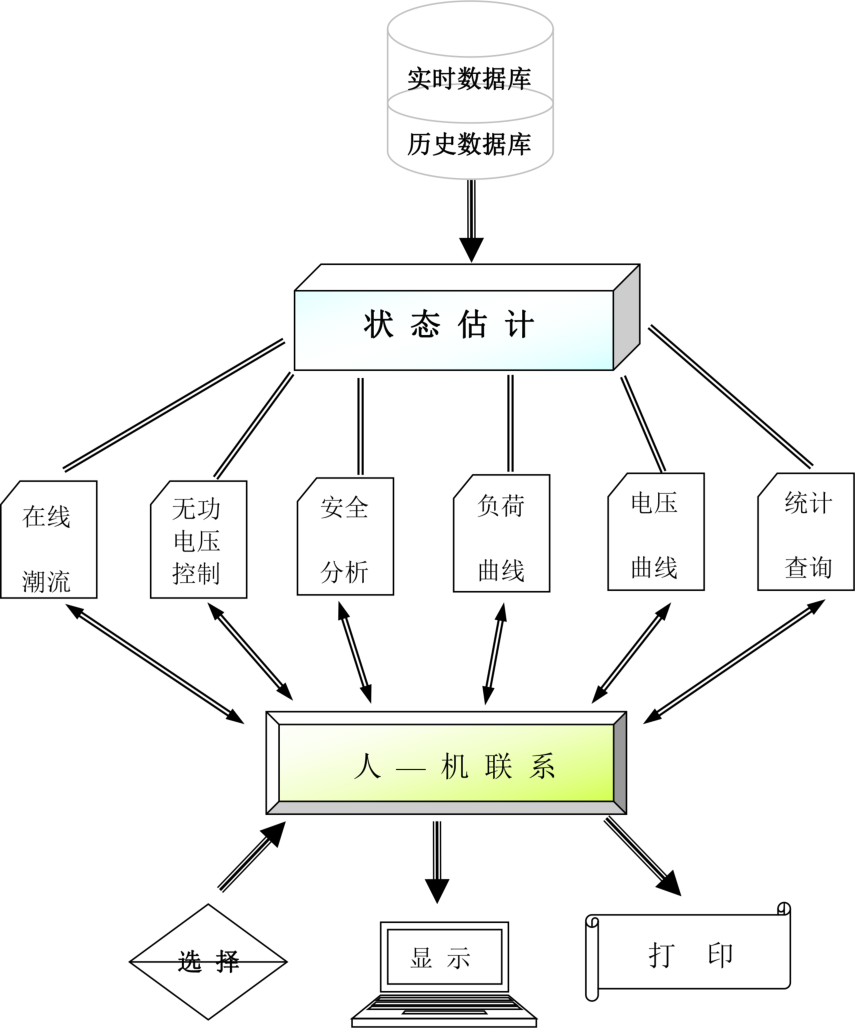
\includegraphics[width=14cm]{2.pdf}
                    \caption{系统功能}
                \end{figure}

            \section{实验内容及数据分析}
                \subsection{启动系统}
                    \textbf{要求:}

                    \textbf{\quad 1) 完成实时运行分析系统的启动,进入“电网实时分析与应用主界面”。}

                    \textbf{\quad 2) 点击进入各功能界面。}

                    \textbf{\quad 3) 记录实际的操作步骤,以及观察到的界面。}\\ 

                    操作过程参考如下:

                    \quad 1) 在 Windows 平台上,双击“电网实时分析”图标,得到如图 4-3 所示系
                    统工作主界面。主界面上列出有关计算和统计内容。

                    \quad 2) 要进行某项计算或统计任务,点击相关项目,即可进入该项任务功能。

                    \quad 3) 点击左下或右下两个图标,即可退出系统。

                    \begin{figure}[htbp]
                        \centering
                        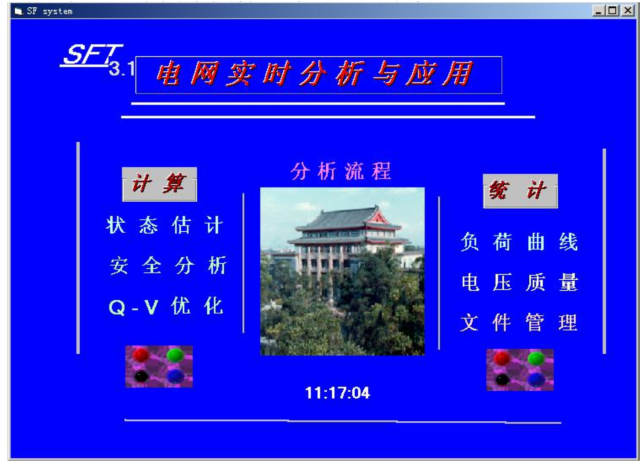
\includegraphics[width=12cm]{3.pdf}
                        \caption{主界面}
                    \end{figure}
                    
                \subsection{状态估计和在线潮流(SE-OLF)}
                    \textbf{要求:}

                    \textbf{\quad 1) 点击进入状态估计和在线潮流功能。}

                    \textbf{\quad 2) 观察记录功能界面。}

                    \textbf{\quad 3) 点击“计算”按钮,进行状态估计和在线潮流计算。}

                    \textbf{\quad 4) 记录实际的操作步骤,记录观察到的显示界面。}

                    \textbf{\quad 5) 记录计算结果,记录结果显示方式。}

                    \textbf{\quad 6) 对功能原理、计算过程和计算结果进行分析。} \\

                    操作过程、说明及结果如下:

                    \quad 1) 进入状态估计和在线潮流功能;

                    \begin{figure}[htbp]
                        \centering
                        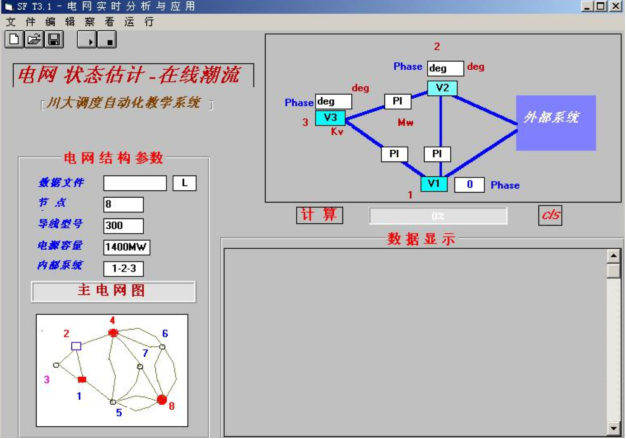
\includegraphics[width=12cm]{4.pdf}
                        \caption{状态估计和在线潮流功能}
                    \end{figure}

                    \quad 2) 观察显示画面的构成;

                    \qquad a.左侧:电网结构图和有关参数;

                    \qquad b.右上:内部系统图形和数据显示;

                    \qquad c.右中:操作按钮和计算进程显示;

                    \qquad d.右下:数据显示窗口。

                    \quad 3) 计算方法和计算结果;

                    \qquad a.点击一次“计算”按钮,则进行一次 SE-OLF 计算

                    \qquad b.点击一次“cls”按钮,则清除所有计算内容显示。

                    \qquad \textbf{c.计算结果如图4.5:}

                    \begin{figure}[htbp]
                        \centering
                        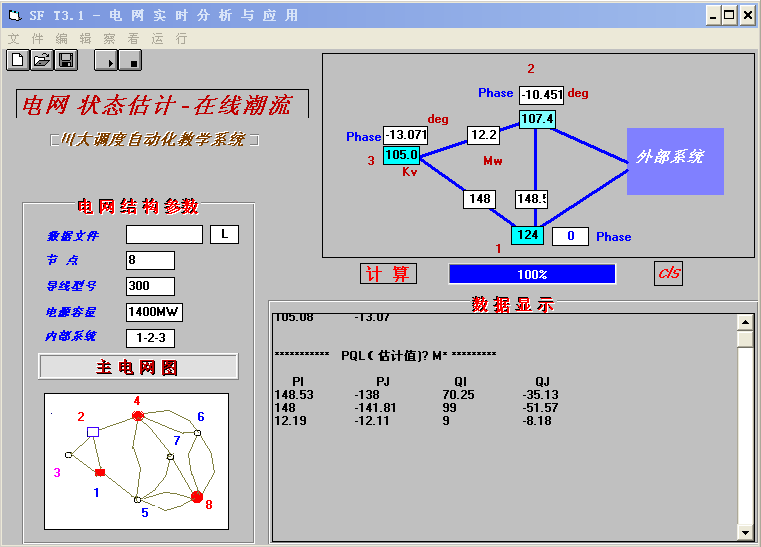
\includegraphics[width=12cm]{5.png}
                        \caption{SE-OLF计算结果}
                    \end{figure}
                    
                    \quad 4) 状态估计-在线潮流是电网实时分析和计算的最基本计算,用来将遥测得到不相容的数据,经过计算处理得到电网的状态估计值:

                    \begin{equation}
                        \begin{aligned}
                            & {\hspace{-0.2cm}\begin{tabular}{p{0.4cm} p{1cm} l}
                                $J$ & $\hat{V}$ & $\hat{\theta}$ \\
                            \end{tabular}} \\
                            X= & {\begin{matrix}
                                1  \\
                                2  \\
                                3  \\
                            \end{matrix}} {\left[\begin{matrix}
                                124 & 0 \\
                                107.46 & -10.45 \\
                                105.08 & -13.07 \\
                            \end{matrix} \right]}
                        \end{aligned}
                    \end{equation}

                    式中,

                    \quad $J$ 为节点(母线)编号;

                    \quad $V$ 为节点电压幅值,单位 kV;

                    \quad $\theta$ 为节点电压相角,以节点 1 为参考节点。

                    同时,可以得到各支路两端的潮流值。通常,支路以两端的节点号来标识。小节点号侧为 $PI$,$QI$,大节点号侧为 $PJ$,$QJ$,并具有“+”或“-”号表示方向。

                    \begin{equation}
                        \begin{aligned}
                            & {\hspace{-0.2cm}\begin{tabular}{p{0.1cm} p{0.3cm} p{1.1cm} p{1cm} p{1cm} l}
                                $I$ & $J$ & $PI$ & $PJ$ & $QI$ & $QJ$ \\
                            \end{tabular}} \\
                            LF= & {\begin{matrix}
                                1 & 2 \\
                                1 & 3 \\
                                2 & 3 \\
                            \end{matrix}} {\left[\begin{matrix}
                                148.53 & -138 & 70.25 & -35.13 \\
                                148 & -141.01 & 99 & -51.57 \\
                                12.19 & -12.11 & 9 & -8.18 \\
                            \end{matrix} \right]}
                        \end{aligned}
                    \end{equation}

                    式中,
                    
                    \quad $PI$,$PJ$ 为有功潮流,$MW$;

                    \quad $QI$,$QJ$ 为无功潮流,$MVar$;

                    \quad “-”表示流出支路。

                \subsection{安全分析(SA)}
                    \textbf{要求:}

                    \textbf{\quad 1) 点击进入安全分析功能。}

                    \textbf{\quad 2) 观察记录功能界面。}

                    \textbf{\quad 3) 点击“计算”按钮,进行安全分析计算。}

                    \textbf{\quad 4) 记录实际的操作步骤,记录观察到的显示界面。}

                    \textbf{\quad 5) 记录计算结果,记录结果显示方式。}

                    \textbf{\quad 6) 对功能原理、计算过程和计算结果进行分析。} \\

                    操作过程、说明及结果参考如下:

                    \quad 1) 进入安全分析功能;

                    \quad 2) 观察显示画面的构成;

                    \qquad a.左侧:电网结构图和有关参数;

                    \qquad b.右上:内部系统图形和数据显示;\quad (支路断开方法)

                    \qquad \quad $\bullet$ \quad 节点或母线显示有电压值;

                    \qquad \quad $\bullet$ \quad 支路显示有有功功率值 PI 和有功功率最大限值 P m

                    \qquad \quad $\bullet$ \quad 支路 P m 键入为 0,表示该支路断开。

                    \qquad c.右中:操作按钮和计算进程显示;

                    \qquad d.右下:数据显示窗口。

                    \begin{figure}[htbp]
                        \centering
                        \includegraphics[width=12cm]{6.pdf}
                        \caption{安全分析功能}
                    \end{figure}

                    3) 计算方法和计算结果;

                    \quad a.点击一次“计算”按钮,则进行一次安全分析 SA 计算;

                    \quad b.点击一次“cls”按钮,则清除所有的内容显示。

                    \quad \textbf{c.计算结果如图4.7:}

                    \begin{figure}[htbp]
                        \centering
                        \includegraphics[width=12cm]{7.png} 
                        \includegraphics[width=12cm]{8.png}
                        \caption{SA计算结果}
                    \end{figure}

                    \begin{figure}[htbp]
                        \centering
                        \includegraphics[width=12cm]{9.png} 
                        \includegraphics[width=12cm]{10.png}
                        \caption{断开“i-j”支路后的SA计算结果}
                    \end{figure}

                    4) 首先进行正常情况计算;

                    正常情况是不断开任何一条支路,可以算出节点电压和支路的潮流。

                    \begin{equation}
                        \begin{aligned}
                            V & = (V_{10},V_{20},V_{30}) \\
                            P & = (P_{120},P_{130},P_{230}) \\
                            Q & = (Q_{120},Q_{130},Q_{230}) 
                        \end{aligned}
                    \end{equation}

                    5) 其次断开“i-j”支路进行计算;

                    计算前,将支路“i-j”的 $P_m$ 置为 0;点击“计算”按钮,可以得到计算结果:

                    \textbf{断开“i-j”支路后的计算结果如图4.8}

                    \quad $\bullet$ \quad 支路 i、j 的潮流为 0;

                    \quad $\bullet$ \quad 其它支路的潮流与该支路 $P_m$ 比较,如大于 $P_m$ ,则为警告状态,用不同颜色显示;
                    
                    \quad $\bullet$ \quad 各节点电压与上限 $V_M$ 和下限 $V_m$ 比较,超过限值,则为警告状态,用不同颜色显示。\\

                    % \begin{figure}[htbp]
                    %     \centering
                    %     \includegraphics[width=12cm]{9.png} 
                    %     \includegraphics[width=12cm]{10.png}
                    %     \caption{断开“i-j”支路后的SA计算结果}
                    % \end{figure}

                    \textbf{实验计算结果为:}

                    \begin{equation}
                        \begin{aligned}
                            & {\hspace{-0.2cm}\begin{tabular}{p{0.1cm} p{0.3cm} p{1.0cm} p{0.9cm} p{0.9cm} p{1cm} p{0.9cm} p{0.9cm} p{0.6cm} p{0.6cm} l}
                                $I$ & $J$ & $V_1$ & $V_2$ & $V_3$ & $P_{12}$ & $Q_{12}$ & $P_{13}$ & $Q_{13}$ & $P_{23}$ & $Q_{23}$ \\
                            \end{tabular}} \\
                                & {\begin{matrix}
                                0 & 0 \\
                                2 & 3 \\
                            \end{matrix}} {\left[\begin{matrix}
                                126.41 & 107.04 & 107.87 & 159.03 & 100.53 & 137.68 & 97.28 & 2.28 & 2.49 \\
                                126.49 & 108.01 & 108.69 & 153.39 & 95.18 & 133.75 & 92.92 & 2.68 & 2.17 \\
                            \end{matrix} \right]}
                        \end{aligned}
                    \end{equation} 

                \subsection{无功-电压优化}
                    \textbf{要求:}

                    \textbf{\quad 1) 点击进入无功-电压优化功能。}

                    \textbf{\quad 2) 观察记录功能界面。}

                    \textbf{\quad 3) 点击“计算”按钮,进行无功-电压优化计算。}

                    \textbf{\quad 4) 记录实际的操作步骤,记录观察到的显示界面。}

                    \textbf{\quad 5) 记录计算结果,记录结果显示方式。}

                    \textbf{\quad 6) 对功能原理、计算过程和计算结果进行分析。} \\

                    操作过程、说明及结果参考如下:

                    1) 进入无功-电压优化调度功能;

                    \begin{figure}[htbp]
                        \centering
                        \includegraphics[width=12cm]{11.png} 
                        \caption{无功-电压优化调度功能}
                    \end{figure}

                    2) 观察显示画面的构成;

                    \quad a.左侧:电网结构图和有关参数;

                    \quad b.右上:内部系统图形和数据显示;
                    
                    \qquad $\bullet$ \quad 右上画面的左上角,用以设定 Pf0(未补偿的负荷功率因数),Pfc(加补偿的负荷功率因数);
                    
                    \qquad $\bullet$ \quad 1\#节点为电源节点,它的电压值$V_1$可以按逆调压要求设定。
                    
                    \quad c.右中:操作按钮和计算进程显示;
                
                    \quad d.右下:数据显示窗口。

                    3) 计算方法和计算结果;

                    \quad a.点击一次“计算”按钮,则进行一次“Q-V”综合计算;
                    
                    \quad b.点击一次“cls”按钮,则清除所有的内容显示。
                    
                    \quad \textbf{c.计算结果如图4.10$\sim$图4.16}

                    \begin{figure}[htbp]
                        \centering
                        \includegraphics[width=12cm]{12.png} 
                        \includegraphics[width=12cm]{13.png} 
                        \caption{$Pfc=0.88$无功-电压优化计算结果}
                    \end{figure}

                    \begin{figure}[htbp]
                        \centering
                        \includegraphics[width=9cm]{14.png} 
                        \includegraphics[width=6cm]{15.png} 
                        \includegraphics[width=6cm]{16.png} 
                        \caption{$Pfc=0.90$无功-电压优化计算结果}
                    \end{figure}

                    \begin{figure}[htbp]
                        \centering
                        \includegraphics[width=9cm]{17.png} 
                        \includegraphics[width=6cm]{18.png} 
                        \includegraphics[width=6cm]{19.png} 
                        \caption{$Pfc=0.92$无功-电压优化计算结果}
                    \end{figure}

                    \begin{figure}[htbp]
                        \centering
                        \includegraphics[width=10cm]{20.png} 
                        \includegraphics[width=6cm]{21.png} 
                        \includegraphics[width=6cm]{22.png} 
                        \caption{$V_1=115V$无功-电压优化计算结果}
                    \end{figure}

                    \begin{figure}[htbp]
                        \centering
                        \includegraphics[width=12cm]{23.png} 
                        \caption{$V_1=118V$无功-电压优化计算结果}
                    \end{figure}

                    \begin{figure}[htbp]
                        \centering
                        \includegraphics[width=12cm]{24.png} 
                        \caption{$V_1=120V$无功-电压优化计算结果}
                    \end{figure}

                    \begin{figure}[htbp]
                        \centering
                        \includegraphics[width=12cm]{25.png} 
                        \caption{$V_1=122V$无功-电压优化计算结果}
                    \end{figure}
                    
                    4) 首先改变负荷无功补偿容量 $Q_C$ ,提高负荷补偿功率因素 Pfc,进行计算;

                    功率因素 Pfc 分别设置为:

                    $$Pfc=\begin{matrix}
                        0.88, & 0.90, & 0.92 \\
                    \end{matrix}$$

                    \quad a.在右上图上,读出 $P_{loss}$ 和各支路的无功潮流 $Q_I$ 及各节点电压;

                    \quad b.在右下图上,读出各补偿容量 $Q_C$ 及各支路的功率损耗 $P_R$ ;
                
                    % \quad c.分析下列
                
                    % \qquad $\bullet$电压质量;
                    
                    % \qquad $\bullet$网损;
                    
                    % \qquad $\bullet$补偿容量。
                    
                    三种指标的综合优化结论。
                    
                    5) 其次改变电源(节点 1)母线电压,进行计算;
                    
                    母线电压分别设置为:

                    $$V_1=\begin{matrix}
                        115, & 118, & 120, & 122 \\
                    \end{matrix}$$

                    \quad 在右上图上读出各节点电压及网损 $P_{loss}$ ; \\
                    
                    % \quad b.选择 Pfc;
                    
                    % \quad c.找出最优策略,使达到
                    
                    % $$Min(Q_c,P_{loss},<V>)$$

                    \textbf{列写出所有情况下的实验计算结果:} 

                    \begin{equation}
                        \begin{aligned}
                            & {\hspace{0.2cm} \begin{tabular}{p{0.3cm} p{1cm} p{0.9cm} p{1cm} p{0.8cm} p{1cm} p{0.7cm} p{0.5cm} p{0.4cm} p{0.4cm} l}
                                $V_I$ & $cos\varphi$ & $V_1$ & $V_2$ & $V_3$ & $Q_{12}$ & $Q_{13}$ & $Q_{23}$ & $Q_{c2}$ & $Q_{c3}$ & $P_{loss}$ 
                            \end{tabular}} \\
                            & {\left[\begin{matrix} 
                                118 & 0.88 & 118.22 & 97.51 & 96.95 & 103.08 & 105.01 & 0.57 & 11 & 12 & 4782.0 \\
                                118 & 0.9 & 118.21 & 97.51 & 96.95 & 97.28 & 99.72 & 0.34 & 20 & 20 & 4702.6 \\
                                118 & 0.92 & 118.93 & 100.35 & 100.00 & 91.1 & 94.09 & 0.07 & 28 & 29 & 4643.8 \\
                                115 & 0.88 & 115.26 & 95.07 & 94.52 & 97.99 & 99.83 & 0.55 & 11 & 12 & 4546.0 \\
                                118 & 0.88 & 118.22 & 97.51 & 96.95 & 103.08 & 105.01 & 0.57 & 11 & 12 & 4782.0 \\
                                120 & 0.88 & 120.19 & 99.14 & 98.56 & 106.55 & 108.54 & 0.59 & 11 & 12 & 4942.9 \\
                                122 & 0.88 & 122.16 & 100.76 & 100.18 & 110.07 & 112.13 & 0.61 & 11 & 12 & 5106.1 \\
                            \end{matrix} \right]}
                        \end{aligned}
                    \end{equation} 

                    \textbf{结论:}
                    
                    \textbf{1.当设置的母线电压$V_I$不变时,功率因数$Pfc$设置的越大,无功补偿越大$Q_c$越大,系统的总损耗$P_{loss}$越小。}

                    \textbf{2.当功率因数$Pfc$不变时,设置的母线电压$V_I$越大,系统的总损耗$P_{loss}$越大,此时无功补偿$Q_c$不变。}

                    \textbf{综合考虑,该系统功率因数$Pfc$设置为0.88,母线电压$V_I$设置为115V时,网损最小。}
                    


                \newpage

                \subsection{负荷曲线 LC}
                    \textbf{要求:}

                    \quad \textbf{1) 点击进入负荷曲线功能。}

                    \quad \textbf{2) 观察记录功能界面。}

                    \quad \textbf{3) 点击相应按钮,进行负荷曲线显示。}

                    \quad \textbf{4) 记录实际的操作步骤,记录观察到的显示界面。}

                    \quad \textbf{5) 记录显示结果及显示方式。}

                    \quad \textbf{6) 对功能原理、显示结果进行分析。} \\

                    操作过程、说明及结果如下:

                    \quad 1) 进入负荷曲线功能;

                    \begin{figure}[htbp]
                        \centering
                        \includegraphics[width=12cm]{26.png} 
                        \caption{负荷曲线功能}
                    \end{figure}

                    \quad 2) 观察显示画面的构成;

                    \quad 3) 了解显示方法;

                    \qquad a.屏幕右侧有三个选键,由鼠标点出选定,即:

                    \qquad \quad $\bullet$ \quad $P_1$ 为节点 1,即电厂输出负荷的曲线;

                    \qquad \quad $\bullet$ \quad $P_2$ 为节点 2,即变电站 2 供给负荷的曲线;

                    \qquad \quad $\bullet$ \quad $P_3$ 为节点 3,即变电站 3 供给负荷的曲线。

                    \qquad \textbf{三条曲线如图4.18$\sim$4.20}

                    \qquad b.鼠标点击“cls”,则可以清除屏幕画出的曲线;

                    \qquad c.鼠标点击“WJ”,则可由输入负荷数据的文件,画出相应的曲线。

                    \qquad d.曲线的黑影差值,用来估计前一日和当日负荷值的差别,$t_0$ 处为左右曲线的断点。

                    \begin{figure}[htbp]
                        \centering
                        \includegraphics[width=11cm]{27.png} 
                        \caption{负荷曲线$P_1$}
                    \end{figure}

                    \begin{figure}[htbp]
                        \centering
                        \includegraphics[width=11cm]{28.png} 
                        \caption{负荷曲线$P_2$}
                    \end{figure}

                    \begin{figure}[htbp]
                        \centering
                        \includegraphics[width=11cm]{29.png} 
                        \caption{负荷曲线$P_3$}
                    \end{figure}

                \newpage

                \subsection{电压曲线 VC}
                    \textbf{要求:}

                    \quad \textbf{1) 点击进入负荷曲线功能。}

                    \quad \textbf{2) 观察记录功能界面。}

                    \quad \textbf{3) 点击相应按钮,进行负荷曲线显示。}

                    \quad \textbf{4) 记录实际的操作步骤,记录观察到的显示界面。}

                    \quad \textbf{5) 记录显示结果及显示方式。}

                    \quad \textbf{6) 对功能原理、显示结果进行分析。} \\

                    操作过程、说明及结果如下:

                    \quad 1) 进入负荷曲线功能;

                    \begin{figure}[htbp]
                        \centering
                        \includegraphics[width=12cm]{30.png} 
                        \caption{电压曲线功能}
                    \end{figure}

                    \quad 2) 观察显示画面的构成;

                    \quad 3) 了解显示方法

                    \qquad a.屏幕右侧有六个选键,由鼠标点击选定,即:

                    \qquad \quad $\bullet$ \quad V1-110 为电厂 1 的 110KV 母线电压;

                    \qquad \quad $\bullet$ \quad V2-110 为变电站 2 的 110KV 的母线电压;

                    \qquad \quad $\bullet$ \quad V3-110 为变电站 3 的 110KV 的母线电压;

                    \qquad \quad $\bullet$ \quad V1-10 为电厂 1 的 10KV 的母线电压;

                    \qquad \quad $\bullet$ \quad V2-10 为变电站 2 的的 10KV 的母线电压;

                    \qquad \quad $\bullet$ \quad V3-10 为变电站 3 的的 10KV 的母线电压。

                    \qquad \textbf{五条曲线如图4.18$\sim$4.20}

                    \qquad b. 鼠标点击“cls”则可以清除屏幕上画出的曲线。

                    \qquad c.鼠标点击“WJ”,则可以由输入的电压数据文件,画出相应的曲线。

                    \begin{figure}[htbp]
                        \centering
                        \includegraphics[width=11cm]{31.png} 
                        \caption{电压曲线V1-110}
                    \end{figure}

                    \begin{figure}[htbp]
                        \centering
                        \includegraphics[width=11cm]{32.png} 
                        \caption{电压曲线V2-110}
                    \end{figure}

                    \begin{figure}[htbp]
                        \centering
                        \includegraphics[width=11cm]{33.png} 
                        \caption{电压曲线V3-110}
                    \end{figure}

                    \begin{figure}[htbp]
                        \centering
                        \includegraphics[width=11cm]{34.png} 
                        \caption{电压曲线V2-10}
                    \end{figure}

                    \begin{figure}[htbp]
                        \centering
                        \includegraphics[width=11cm]{35.png} 
                        \caption{电压曲线V3-10}
                    \end{figure}


            \section{总结和思考}
                通过本次实验,我充分认识到了能量管理的实时运行分析功能在调度自动化系统中的重要作用。在我们课堂的学习当中,
                都是用人工地方式进行潮流计算。但是在实际电力系统运行中,若需要实时调度,则必须使用计算机迅速地计算出潮流数据,以供调度员参考。
                尽管本次实验所模拟的系统是一个简单的小系统,但是通过对它的学习,我们可以充分掌握能量管理实施运行分析的基本功能和操作,对于电网的实施状态
                及其变化有了直观的认识,为我们今后在工作中的深入学习打下良好的基础。


\end{document}